\documentclass{article}

\usepackage{arxiv}

\usepackage[utf8]{inputenc} % allow utf-8 input
\usepackage[T1]{fontenc}    % use 8-bit T1 fonts
\usepackage{hyperref}       % hyperlinks
\usepackage{url}            % simple URL typesetting
\usepackage{booktabs}       % professional-quality tables
\usepackage{amsfonts}       % blackboard math symbols
\usepackage{amsmath}
\usepackage{nicefrac}       % compact symbols for 1/2, etc.
\usepackage{microtype}      % microtypography
\usepackage{cleveref}       % smart cross-referencing
\usepackage{lipsum}         % Can be removed after putting your text content
\usepackage{graphicx}
\usepackage{natbib}
\usepackage{doi}
\usepackage{placeins}

\title{LLM-Based Agent Assistants for Supporting Knowledge-Intensive Processes: A Detailed Survey of Components and Potential Methods } % LLM-Based Agent Assistants: A Detailed Survey of Components and Potential Methods for Supporting Knowledge-Intensive Processes in the Enterprise

% Here you can change the date presented in the paper title
%\date{September 9, 1985}
% Or remove it
%\date{}

\newif\ifuniqueAffiliation
% Comment to use multiple affiliations variant of author block 
\uniqueAffiliationtrue

\ifuniqueAffiliation % Standard variant of author block
%\author{ %\href{https://orcid.org/0000-0000-0000-0000}
%	{\hspace{1mm}David S.~Hippocampus}\thanks{Use footnote for providing further
%		information about author (webpage, alternative
%		address)---\emph{not} for acknowledging funding agencies.} \\
%	Department of Computer Science\\
%	Cranberry-Lemon University\\
%	Pittsburgh, PA 15213 \\
%	\texttt{hippo@cs.cranberry-lemon.edu} \\
	\author{ %\href{https://orcid.org/0000-0000-0000-0000}
		{\hspace{1mm}Aline Dobrovsky}\\
		Department of Artificial Intelligence and Cybersecurity\\
		University of Klagenfurt\\
		9020 Klagenfurt, Austria \\
		\texttt{aldobrovsky@edu.aau.at} \\
	%% examples of more authors
	\And
	%\href{https://orcid.org/0000-0000-0000-0000}
	{%\includegraphics[scale=0.06]{orcid.pdf}
		\hspace{1mm} ToDo Ask Co-Author} \\
	Department of Artificial Intelligence and Cybersecurity\\
	University of Klagenfurt\\
	9020 Klagenfurt, Austria\\
	\texttt{...} \\
	%% \AND
	%% Coauthor \\
	%% Affiliation \\
	%% Address \\
	%% \texttt{email} \\
	%% \And
	%% Coauthor \\
	%% Affiliation \\
	%% Address \\
	%% \texttt{email} \\
	%% \And
	%% Coauthor \\
	%% Affiliation \\
	%% Address \\
	%% \texttt{email} \\
}
\else
% Multiple affiliations variant of author block
\usepackage{authblk}
\renewcommand\Authfont{\bfseries}
\setlength{\affilsep}{0em}
% box is needed for correct spacing with authblk
\newbox{\orcid}\sbox{\orcid}{%\includegraphics[scale=0.06]{orcid.pdf}
} 
\author[1]{%
	\href{https://orcid.org/0000-0000-0000-0000}{\usebox{\orcid}\hspace{1mm}David S.~Hippocampus\thanks{\texttt{hippo@cs.cranberry-lemon.edu}}}%
}
\author[1,2]{%
	\href{https://orcid.org/0000-0000-0000-0000}{\usebox{\orcid}\hspace{1mm}Elias D.~Striatum\thanks{\texttt{stariate@ee.mount-sheikh.edu}}}%
}
\affil[1]{Department of Computer Science, Cranberry-Lemon University, Pittsburgh, PA 15213}
\affil[2]{Department of Electrical Engineering, Mount-Sheikh University, Santa Narimana, Levand}
\fi

% Uncomment to override  the `A preprint' in the header
%TODO
\renewcommand{\headeright}{}
\renewcommand{\undertitle}{}
\renewcommand{\shorttitle}{LLM-Based Agent Assistants: A Detailed Survey of Components and Potential Methods}
%LLM-Based Agent Assistants: A Detailed Survey of Components and Potential Methods for Supporting Knowledge-Intensive Processes in the Enterprise

%Numbering also for paragraphs
%\renewcommand{\theparagraph}{\S\arabic{paragraph}}
\setcounter{secnumdepth}{5}
%Paragraphs in table of contents
\setcounter{tocdepth}{5}

%%% Add PDF metadata to help others organize their library
%%% Once the PDF is generated, you can check the metadata with
%%% $ pdfinfo template.pdf
%TODO
\hypersetup{
pdftitle={LLM-Based Agent Assistants: A Detailed Survey of Components and Potential Methods for Supporting Knowledge-Intensive Processes in the Enterprise},
pdfsubject={q-bio.NC, q-bio.QM},
pdfauthor={Aline~Dobrovsky, .},
pdfkeywords={Large Language Models, Intelligent Agents, ...},
}

\begin{document}
\maketitle

\begin{abstract}
	TODO
%	survey
%	identify
%	parallels
%	dimensions
%	characterize, identify
%	for further research
%	
%	The idea of...agents...
%	complex...
%	widely recognized
%	tedious, time consuming, expensive,...
%	automation
%	comprehensive overview
%	discuss key issues
\end{abstract}

\keywords{Large Language Models \and Intelligent Agents \and ...}


\section{Introduction}
DRAFT: ONLY NOTES

General Intro of idea, notes: 
\cite{wooldridge_intelligent_1995} in 1995 already describe the vision of a personal digital assistant, that among other activities atonomously fetches and aufbereiten interesting information and performs as assitant in many...information domains...interacts with different systems ... all based on the notion of a software agent
\cite{goos_intelligent_2002} or in 2002 a internet search assistant that autonomously queries different ressources and sythesizes information

INTRO: SUCCESSES OF LLMS 
%goal of LM: next word prediction?
%before: search, keyword, or LLM

LLMs: towards human-level intelligence (refer to tests/benchmarks) 
LLMs good at: natural language generation, question answering, summarization
interaction, emergent: reasoning and planning (chain of thought prompting -thin step by step)
many improvements last few years, 
remarkably effective

\cite{xi_rise_2023} LLMs have demonstrated powerful capabilities in knowledge acquisition, instruction comprehension, generalization, planning, and reasoning, while displaying effective natural language interactions with human

\cite{valmeekam_planning_2023} "no exaggeration to say that transformer-based large language models (LLMs) have revolutionized the field of natural language processing (NLP)"
original: sequence completion, but claims of emergent capabilities (reasoning, planning)

\cite{bubeck_sparks_2023} "GPT-4 can solve novel and difficult tasks that span mathematics, coding, vision, medicine, law, psychology and more, without needing any special prompting. Moreover, in all of these tasks, GPT-4’s performance is strikingly close to human-level performance"


INTRO: LIMITS OF LLMS REGARDING REASONING/PLANNING
%key challenges, main issues

Problem/issue related to use case: recent data, domain knowledge - hallucinations, LLM on their own: only knowledge based on training data, cannot use "local" specialised data
+ multi-modality,might need..but..., custom processes, not enough data for training/fine-tuning

Addressed issues
Complex tasks may require multi-step reasoning and specific tools
LLMs tend to produce hallucinations
Formal approaches require complete and accurate formal descriptions
Specialised tools require specific formal input formats 

Problem/issues of planning and reasoning: complex inputs, requiring advanced reasoning, multi-step questions requiring multi-step reasoning instead of input/output (+ also add that there's RAG but does ot change the single step approach), LLM specialised in text completion not planning/no world model besides statistical/word similarity, LLM direct input-output

\cite{shen_hugginggpt_2023} challenges: LLMs (not multimodal)  limited to text input and text generation, real-world scenarios: complex tasks consisting of multiple sub-tasks, LLMs in specialized...weaker than expert/fine-tuned models
Two research directions: multimodal models + models using external tools

\cite{bubeck_sparks_2023} LLM limitation: "architecture does not allow for an “inner dialogue” or a “scratchpad”, beyond its internal representations, that could enable it to perform multi-step computations or store intermediate results." because of next word prediction only one direction..forward not in training data...
planning: needs to know in first steps hat last step will be to create consistent answer. Humans can backtrack

LLMs are ill-equipped for naive long-term planning since managing an extensive context over multiple steps is complex and resource-consuming (Silver et al., 2022; Liu et al., 2023) \cite{silver_generalized_2023}?? ArXiv, abs/2304.11477 \cite{liu_llmp_2023}

Problem: Want to solve every problem with a LLM: Swiss army knife, From good one tool (complete/predict sentences/words, bloated - can do everything, requiring different modalities, specialized information or tools would be better

INTRO: LLM-BASED AGENT APPROACH
% Agent approach, definition
%Therefore: agent approach 

Naming/Definition: LLM-based agents, LLM agents, ...

objective/goal: solve complex tasks, some degree of autonomous behaviour
reasoning use to break down complex tasks/queries to simpler steps
break down complex goals/tasks/issue into manageable simper steps/tasks
Answering complex queries with LLMs, involving multiple steps, solve a complex task involving several steps
multi-step reasoning
Employ a LLM as controller for an AI assistant agent
Process complex and vague natural language questions
Plan sequence of less complex tasks to solve overall task 
Autonomously use specialized tools without requiring manual queries
idea: agents planning which use LLM as controller/main aspect/ core
Answer complex questions or solve complex tasks
Exploit LLM capabilities with natural language, interaction and reasoning
less hallucinations?accuracy? relevance?!
Assistant: automated communication with other systems (find documents, edit document content, (use as context within model)
Integration, automatization other services (Ai services, databases,..)
LLM controller that manages specialised models and offers a natural language interface
Task planning, model selection and control, result summarisation
Write tasks, planning, select tools, generate prompts/queries from tasks
Summarise eg results from elastic search query. References must be included!
Autonomous, goal-directed behaviour

Answer queries using local data
Find correct and relevant data/content and synthesize
Generate explanations for engineers and clients (+ save time)
Client: Writes observations, gets feedback of what could be failure and/or if it should be submitted
Engineer: existing/past cases with similarities, optionally suggestions about cause (of possible causes described in documents)
Professional assistant
Connect LLM and information systems
Retain intellectual property
Specialised models, modularity
User interface: NLP, natural, not specialised (like SQL database query)

Use LLM: natural language interface, Input: text (sometimes multimodal)
LLM: controller/main controller/brain
consists of: a core, mainly with LLM, main coordination, planning, tool usage, memory + user request
use LLM as core, computation
using prompts to direct/steer behaviour
language: understand instructions
natural language interface, intuitive interaction
reasoning capabilities??


LLM capability? complex tasks -> break into manageable subtasks and reason/execute... to solve overall task, multi-step 
planning
break complex task into subtask and address each on their own, by using tools, operation flow/steps

Add: equip LLMs with an expanded perception space and action space, utilize external tools, external resources 
combination of LLM with planning, memory and tool usage
access to API: information retrieval, database,...eventually: tool to interpret data, produce graphic or similar (eg library, python library like pandas?)
recent knowledge not trained on
specific knowledge, domain knowledge
thinking iteratively
specialized tools/plugins

\cite{shen_hugginggpt_2023} "LLMs could act as a controller to manage existing AI models to solve complicated AI tasks and language could be a generic interface to empower this" "select models according to their function descriptions available in Hugging Face, execute each subtask with the selected AI model, and summarize the response according to the execution results"
"Language serves as an interface for LLMs"
"the key point is how to choose suitable middleware to bridge the connections between LLMs and AI models"
task planning, model selection, task execution, response generation



\cite{dagan_dynamic_2023} despite prompting techniques like Chain of thought (REF), self-consistency (REF) and ReAct(F), limits of context window, hallucinations
"LLMs in Planning and Reasoning In contrast to symbolic planners, LLMs have shown promise in adapting to noisy planning and reasoning tasks through various methods. Some general approaches such as Chain-of-Thought (Wei et al., 2022), Self-Consistency (Wang et al., 2023b), and Reasoning via Planning (Hao et al., 2023) augment the context with a reasoning trace that the LLM generates to improve its final prediction."
"But symbolic planners require problem and domain descriptions as prerequisites (McDermott, 2000), which hampers their applicability in real-world scenarios where it may be infeasible to achieve these high informational demands."


%misalignemnt: learned/pre-trained knowledge and enviornment rules /process/..., also limits of environment

INTRO: SCOPE OF ARTICLE
%Scope
%motivation behind this survey
%aims at
%point out
%key contribution of this survey
%identify..dimensions, categories, categorize
%positioning ...along...

What this article's scope is/what it concentrates on and what not
For knowledge workers/work?
Personal assistants??
relevant information/answers!
here approaches with planning AND tool, also some promising approaches not directly using tools but act in simulation environment but nonetheless promising for also this explicit tool use case
here: task/goal-oriented agents
analyse prompt, extract goal, parameters etc, plan, execute actions and result
cover the base...ideas/approaches, not collect every single publication, anyhow already fast paced area
potential for practical application
but also mention some open issues and potential for further research
foremost..of practical use, help support to select
reader can identify opportunities for future research by...looking at..less common/never tried/novel combinations
many existing... continuously new proposals/papers,...
important to...overview, catalogue,...offer comprehensive resource for those... interested in...
in order to provide this survey...cover publications...searched for...
focus: agent architecture/methods/parts, o be able to ... their advantages/disadvantages
techniques differ
overview over as many as possible
group in appropriate categories
full discussion of approaches in the respective papers
design: to maximise, find best, find suitable architecture/components,...
here: literature research, literature review and critical analysis

Research question: What do we do not know yet?
Here: which approaches exist? How can they be classified
And then which aspects/designs are appropriate for which tasks with focus ion complex queries like/similar as FA 
goals and methodology
literature analysis

NOT:
fine-tuning
not finetuning, depends on expected use case: using a trained LLM on very specific domain data, where finetuning would be not or barely possible (effort, cost-effectiveness?, generalizability/catastrophic forgetting), needs specialized data, labelled?
also no additional instruction fine-tuning as agent
NOT papers with special application areas, like agent for XY, Code commenting etc, where paper not about specifics of agent structure, trading,...playing specific game..?

literature search until: 11.03.2024
updated literature search: 21.04.2024
Methodology:
Search: google scholar, https://dl.acm.org/, https://ieeexplore.ieee.org/, https://dblp.org/, following references, Connected papers https://www.connectedpapers.com/
TODO: mention initial keywords used for search?


%overview/structure
TODO: STRUCTURE OUTLINE


\section{Related Work}
\label{sec:related}
INITIAL FORMULATION

%searched for surveys, google scholar: Large language model agent planning survey
%ACM digital library, IEEE explore, https://dblp.org/
%14 items, thereof: 2 blogposts, 11 articles
%thereof in journals/conferences/peer-reviewed: 2

This section introduces, discusses, and presents related literature surveys that discuss characteristics and develop taxonomies for LLM-based agents. It includes nomenclature and what others have identified as the main characteristics and main components of LLM-based agents. Given the novelty of this field, with publications appearing only since 2023, peer-reviewed literature has been complemented by preprints and blog postings. The material has been ordered according to publication date. 

%%%%%%%%%%%%%%%%%%%%%%%%%%%%%%%%%%%%%%%%%%%%%%%%%%%%%%%%%%%
The authors of \cite{mialon_augmented_2023} conducted a survey of 'augmented language models' (LLMs), where LLMs, originally trained with the missing token prediction objective, are augmented with additional abilities. These abilities include reasoning, the ability to decompose tasks into subtasks (planning), information retrieval (RAG), and the ability to use tools and call external modules. The objective is to enhance the otherwise limited context of LLMs. The authors discuss prompting and finetuning techniques for reasoning tasks, tool usage and  rewards from the environment and humans for reinforcement learning, and they discuss potential issues within each category. 
%In comparison to this work, no fine-grained classification and no analysis of different techniques.
% : LM improve context with RAG or with reasoning strategies or external tools
%What they do: how LLM with missing token objective can be enhanced with reasoning capabilitiey and ability to use tools, 
%clasification : reasoning, interaction with external tools, implementation of reasoning and tool usage, also mention integration of symbolic modules (in using tools), lerning to reason and use tools
%What they don't: Reasoning: mainly prompting techniques and finetuning to reasoning tasks, mention general possible problems per category, but no analysis of the techniques
%%%%%%%%%%%%%%%%%%%%%%%%%%%%%%%%%%%%%%%%%%%%%%%%%%%%%%%%%%%
%BLOG 23.06.2023, added here: 19.02.24
The authors of \cite{weng_llm_2023} define 'LLM-Powered Autonomous Agents' as agents that utilise an LLM as their core controller, in conjunction with further components including planning, memory, action, and tools. They describe some illustrative approaches that demonstrate the realisation of these components. %without classification
%and do not introduce an explicit classification with analysis of techniques.
%What they do: agent system overview with 4 components of an agent, mention some exemplary approaches covering realising the different components
%What they don't: some exemplary approaches, that also cover some distinct techniques, but no explicit classification of different techniques, no analysis of techniques
%%%%%%%%%%%%%%%%%%%%%%%%%%%%%%%%%%%%%%%%%%%%%%%%%%%%%%%%%%%
%PREPRINT 11.08.2023
%BOLAA: BENCHMARKING AND ORCHESTRATING LLM-AUGMENTED AUTONOMOUS AGENTS, LAA
\cite{liu_bolaa_2023} present a discussion of "LLM-augmented Autonomous Agents," which extend the capabilities of LLM for the purposes of action execution. They further consider the possibilities of environment interaction and the use of memory. The authors discuss different agent architectures for solo agents, including the use of LLMs for iterative planning with different prompting techniques, and the possibility of orchestrating multiple agents. They compare  performances of six different architectures with different LLMs and argue that multiple coordinated agents solve complex tasks better. 
%They also present some selected approaches for testing.
%, no comprehensive overview over different techniques for the single components.
%What they do: comparison of LAA, multiple agents with a controller, suggestions for designing LAA architectures and LLM choice, argue that multiple coordinated agents solve complex tasks better, compare LAA performances for 6 different architectures with different LLMs + introduce approach to orchestrate a multi-agent strategy
%architectures comprise useLLM for itererative planning with different prompting techniques, on selected benchmarks
%What they don't: no wide overview over different techniques but rather testing some selected own architectures

%%%%%%%%%%%%%%%%%%%%%%%%%%%%%%%%%%%%%%%%%%%%%%%%%%%%%%%%%%%
%\cite{wang_survey_2023} --good, preprint: 07.09.2023, , peer-reveiwed version: \cite{wang_survey_2024}
%A Survey on Large Language Model based Autonomous Agents
\cite{wang_survey_2024} present a framework for designing 'LLM-based autonomous agents' architectures consisting of four modules. The profile module describes the role of the agent and the possible contents and generation strategies of agent profiles. The memory component can include different memory structures, formats and operations; and the planning and action components. The planning component is distinguished according to whether it employs feedback. Planning comprises single-path reasoning, multi-path reasoning, or an external planner. Feedback can be distinguished into environmental, human, or model-derived feedback. The action component is further divided into four categories: action target, action production, action space, and action impact. The authors outline various techniques that can be employed within the framework's components, and present potential applications and evaluation strategies. 
%In difference to this article here: no profile as rarely used, rather for multiagent approaches, different classification, especially planing anderes aufgeteilt, separation of feedback tehcniques and more fine-grained
%examine compare characteristics
%, taxonomies for existing studies, architecture/modules with many components...
%What they don't: Environment?? External knowledge sources??
%They discuss profile but only one approach (MetaGPT) uses this at all?? Why discussing and proposing techniques without existing work/proof of concept? Mixing Agentapproaches with general techniques not (ye) used in any agent (e.g. Reflective linguistic programming)
%always refers to how humans think but without reference etc, we: only existing/PoC
%List single/multi path reasoning as planning without feedback but  can't this be combined/intertwined with feedback?
%Not how planning? complete versus iterative Not single multi agent not plan properties. No analysis of methods.
%We: explain techniques + theoretical backgrund more in detail. Separate planning itself and feedback functionality that can be applied additionaly to different planning techniques
%Explain application areas but also with "agents" not adhering to definition?
%sometimes quite general
%Are they the only ones to list "Profile" as own module?
%Different: categories structured differently. do not assume profiling module necessary, just another prompting method?
%Application areas and evaluation methods...structures..differently?
%%%%%%%%%%%%%%%%%%%%%%%%%%%%%%%%%%%%%%%%%%%%%%%%%%%%%%%%%%%
%PREPRINT 19.09.2023
\cite{xi_rise_2023} discuss the origin of the 'LLM-based agents' concept and explain the suitability of LLMs as a foundation for agents. They propose a general framework for LLM-based agents with three main components.
The brain component includes the agent's knowledge and memory, and it makes decisions via planning or reasoning. The perception component processes environmental inputs and the action component expands the action space of LLMs by allowing the output of text, the use of tools and the execution of embodied actions. They mention three different types of applications: single agent, multi-agent and human-agent cooperation, explain the different, exemplary techniques for each of the components in their typology. 

%agent society
%practical applications of LLM-based agents
%agent within environment
%description appropriate LLMs for Tasks like natural language interaction with human conversation, generlization, ...language generation, reasoning, planning
%typology of applications
%What they don't: for concepts of components only very coarse classification into the three basic agent parts perception, action, brain; summary of different approaches in their typology areas, eg references to approaches of plan formulation , but plan formulation is only category, no distinction of different smethods, no analysis of the techniques

%%%%%%%%%%%%%%%%%%%%%%%%%%%%%%%%%%%%%%%%%%%%%%%%%%%%%%%%%%%
%\cite{zhao_-depth_2023} ONLY PREPRINT 23.09.2023
%An In-depth Survey of Large Language Model-based Artificial Intelligence Agents

\cite{zhao_-depth_2023} survey 'LLM-based AI agents', where the LLM is used as the agent's brain. They introduce an agent classification scheme, consist of three components. The planning component is based on LLM inference and consists of task compositions and self-reflection. The memory component consists of sensory memory as input embedding, the short-term, temporary memory and the long-term stored memory. The third component is tool integration for LLM usage. They further mention general application categories for LLM-based AI agents, including chatbots, games, coding, design, research, collaboration, and general purpose applications. 
%What they do: difference "traditional AI agents" and "LLM-based AI agents"  key components of AI agents, classification scheme. Categories of Application
%What they don't: rather general introduction of the 3 components, no detailed classification (except maybe a bit for memroy). Not really in-depth.
%%%%%%%%%%%%%%%%%%%%%%%%%%%%%%%%%%%%%%%%%%%%%%%%%%%%%%%%%%%
%PREPRINT 27.09.2023
\cite{sumers_cognitive_2023} are concerned with 'cognitive language agents', propose a framework for 'Cognitive Architectures for Language Agents (CoALA)' and and provide a retrospective analysis of this concept in the context of broader AI history. The article describes the structure of a cognitive language agent, which comprises three main components. The information storage contains a working and a long-term memory, the action space
offers internal and external actions, and  the decision making procedure consists of an interactive loop of planning and action execution.

%LLMs: select action, reason, manage memory
%internal memory
%environment
%cognitive language agent: anvironment with observations, actions, memory and reasoning
%CoALA three main dimensions:
%information storage (working and long-term memory)
%action space (internal and external actions)
%decision making procedure (interactive loop of planning and execution)
%What they do: , retrospecitvely survey work in context of broader AI history and identification of future directions
%theoretical framework and use to organize empirical work?, draw parallels to production systems
%What they don't: fit everything into their concept, works but nuances of different techniques not visible, no analysis/evaluation of techniques, only outlook to possible beneficial approaches,. Show some selected example and how they fir into their CoALA, more than half the apper definitions references to very general topics and history.....

%%%%%%%%%%%%%%%%%%%%%%%%%%%%%%%%%%%%%%%%%%%%%%%%%%%%%%%%%%%
%PEER REVIEWED 2023 (arxcie: 05.10.2023) GOOD ARCHITECTURE
In \cite{handler_taxonomy_2023} the author introduces a multi-dimensional taxonomy for 'autonomous LLM-powered multi-agent' architectures with focus on the balancing of autonomy and alignment of agents. An agent is defined as an LLM with a specific role and access to external resources, such as data, tools, or models. The author describes the core characteristics of agent architectures, including goal-driven task management, the LLM at the core of agents, agent collaboration, context interaction, and the balancing of autonomy (adaptive and self-organising aspects) and alignment (real-time responsive and user-guided aspects). It then presents a taxonomic classification of some selected representative LLM-powered multi-agent systems. 
%divide and conquer: decompose task and assign to specialized agents. 
%architecture: context interaction, multi-agent collaboration, agent composition, goal-driven task management
%autonomy: static, adaptive, self-organizing
%alignment: real-time responsive, user-guided, integrated
%goal-driven task management: decomposition, LLMs
%multi-agent collab: message exchange
%context interaction: contextual (external) ressources
%autonomy and alignment: customization, and generic alignment, autonomy: more or elss strict decision-making with parameters, possibly adaptable
%What they do: multi-dimensional taxonomy,  balance between autonomy and alignment, taxonomic classification of selected representative LLM-powered multi-agent systems with reference to balance between autonomy and alignment
%explain taxonomy
%assessment of selected systems: alignemtn and autonomy for viewpoint-specific aspects
%What they don't: nor eal survey, developed taxonomy and selected approaches to prrof its usability
%concentrate on Multi-agent architectures!
%%%%%%%%%%%%%%%%%%%%%%%%%%%%%%%%%%%%%%%%%%%%%%%%%%%%%%%%%%%
%\cite{yule_wang_complete_2023}  A Complete Guide to LLMs-based Autonomous Agents (Part I)
%BLOG retrieved: 03.02.2024, date: 10.10.2023
The blog post \cite{yule_wang_complete_2023} discusses the critical components of LLMs as a brain, memory, and external tool and data resources. It explains the principles of LLM-based agents, including the structure and program flow of an agent, and describes prompting techniques used forthe part of reasoning, task decomposition, and planning. 
%Agent perception: inputs, sensors/tools, action: text, tools, embodiment 
%%brain: LLM is brain,  storage with memory and knowledge and decision making with planning, reasoning
%LLMbreaks down task into substeps, reasoning, actioning, evaluation, suzmmarizing
%+external ressources: memory, toold
%can be unimodal (text input/ouput) or multimodal
%components connected by "traditional rule-based programming"
%input: user command + instructions + prior conversations + record of previous steps (actions and observations)
%output text, also specilized format like json possible
%memory of previous plans
%how to deal with memory vs token constraint: memory buffer, memory summarization, structured memory storage
%external data resources: RAG
%program flow for each sub-step: reasoning, employment of external tools/resources, result evaluation, refine sub-step
%Evaluator for evaluation sub-steps, self-feedback
%LLM for:
%planner, reasoner, actioner, RAG, evaluator, memory
%What they do: explanation of principles of LLM-based agent including of aufbau und program flow agent and prompting techniques used 
%explain prompting techniques used for reasoning/decomposition/planning, possible parts for construction
%What they don't: concentrate on on prompingt/LLM only? trennen planning and reasoning capabilities (planning, reasoning on specific task/or to select one of several possible tasks), no survey over existing papers of concepts/implementations of agents, no evaluation of components, no discussion of approaches..with..symbolic, its only a blog, no taxonomy/categories
%%%%%%%%%%%%%%%%%%%%%%%%%%%%%%%%%%%%%%%%%%%%%%%%%%%%%%%%%%%
%\cite{zhang_igniting_2023} PREPRINT 20.11.2023
%Igniting Language Intelligence: The Hitchhiker’s Guide From Chain-of-Thought Reasoning to Language Agents
%autonomous language agents
The article \cite{zhang_igniting_2023} focuses on the prompt-based reasoning process known as Chain-of-thoughts(CoT) in language agents and its potential. It outlines the fundamentals of CoT, the evolution of CoT approaches and discuss advantages of CoT and effective use cases. Furthermore, the authors provide an overview of some selected agents approaches using CoT. 

%prompting pattern, reasoning format (unstructured natural language, to structured), application scenario
%CoT: decosntruct into sub-problems
%autonomous agents and communicative agents
%Langage agent plan,decision, contsol, memory, state action???  + interaction with tools, interaction with environment
%
%What they do: survey paper, focus on CoT reasoning approach, its foundations,paradigm shift in CoT, language agents based on CoT, evolution of CoT, advantages of using CoT, when CoT is effective, overview over some selected agents approaches (that use CoT??? this is not referenced here!!!)
%What they don't: focus only on CoT reasoning approach

%%%%%%%%%%%%%%%%%%%%%%%%%%%%%%%%%%%%%%%%
%\cite{muthusamy_towards_2023} IBM paper, accepted in Findings of the {Association} for {Computational} {Linguistics}: {EMNLP} 2023
%Towards large language model-based personal agents in the enterprise: Current trends and open problems

The paper \cite{muthusamy_towards_2023} discusses 'LLM-based personal agents' as personal agents in the enterprise. They characterise LLM-based agents as designed to work with complex goals, use a LLM as an orchestrator or brain and have flexible tool access. The agents' task is to identify a sequence of actions that is composed of external tools. The paper goes on to discuss the disadvantages of LLM-based agents in the enterprise and the current shortcomings of this technology. These include the fact that they are brittle to input changes, sensitive to the LLM used, and can get stuck in reasoning loops. Furthermore, they LLMs be slow and expensive to run, and tool usage can emit side effects. 
%complex goals, pluggable tools/APIs
%LLM as orchestrator/brain of autonomous agents, high-level goals
%sequence of actions = compose external tools
%discussthereadinessof LLM-basedautonomousagentsforenterpriseapplications
%agents/tool composers
%integration of APIs with LLMs
%What they do: disadvantages of LLM based agent/current shortcomings: brittle to input changes, can get stuck in reasoning loops, research challenges
%personal assistant in enterprise setting
%Limitations: stuck in loops decomposing tasks, brittleness/inconsistent behaviour, sensitive to used LLM, slow, expensive (LLM calls), tools can have side-effects, limitations in reasoning"currentlimitationsofLLM-basedagentspresentroadblocksto adoptionforenterpriseusecases,whererisk,cost, androbustnessarecriticalissues"
%agent domains: Domain-agnostic, robotic, others
%discuss metrics and benchmarks
%real applications in enterprise setting - limitations of current approaches for this setting
%What they don't: 
%%%%%%%%%%%%%%%%%%%%%%%%%%%%%%%%%%%%%%%%%%%%%%%%%%%%%%%%%%%
%\cite{cheng_exploring_2024} PREPRINT 07.01.2024
%EXPLORING LARGE LANGUAGE MODEL BASED INTELLIGENT AGENTS: DEFINITIONS, METHODS, AND PROSPECTS
The paper \cite{cheng_exploring_2024} explores the concept of 'LLM-based intelligent agents'. It offers a comprehensive overview of the current research in this field, including definitions, agent components, single and multiagent approaches, datasets, application scenarios, performance evaluations, and prospects for future applications. 
The proposed framework for LLM-based agents comprises of five key components. The planning component can be realised by in-context learning methods (via prompting), external methods (like PDDL), and multi-stage methods. The memory component encompasses short-term memory, long-term memory and memory retrieval methods. The rethinking component encompasses different rethinking capabilities, such as in-context learning (prompting), supervised learning, reinforcement learning, and modular coordination. The environment component is divided into possible general application areas. The action component encompasses tool employment, tool planning and tool creation. The authors also offer a typology for multiagent approaches. Agent relationships can be cooperative, competitive, mixed or hierarchical, planning types can be centralized or decentralised multiagent planning end diverse methods exist to potentially enhance communication efficiency. 
%What they do: survey of current research in LLM-based agents, definitions, components, single and multiagent, datasets, applciation scenarios, performance evalutation, prospect applications
%system overview includes: Field, (training), environment (text, game,...), Data, evaluation, modality (text/multimodal), feedback, tool planning, review???(RL/ICL/NONE???)
%What they don't: net very detailed regarding the methods, eg general overview over in-context learning=prompting or PDDL possibiliy, no analysis?, was most of space with very general theory introduction and general prospective applciations. No in-depth explanation of the methods
%%%%%%%%%%%%%%%%%%%%%%%%%%%%%%%%%%%%%%%

The authors of \cite{huang_understanding_2024} concentrate on LLM-based agents planning. They provide a detailed analysis of planning abilities, advantages and limitations, and an evaluation of representative methods on four benchmarks. The authors categorise planning in five distinct areas: task decomposition, which involves breaking down a task into smaller subtasks and conduct sequential planning; multi-plan selection, which entails selecting one of several potential plans; external module-aided planning, which leverages external modules to assist in planning; reflection and refinement, which involves analysing and modifying a plan based on feedback; and memory-augmented planning, which utilises memory to enhance the planning process.

%discussion of (dis)advantages of representative approaches for each category
%possibilities of evaluating planning capabilities
%What they don't: no tool usage discussion

%LLMs as planning modules of autonomous agents
%overview of LLM-based agents planning
%Planning: task decompostion, plan selection, external module, reflection, memory



DRAFT- THIS SURVEY (without discrimination related work!): 
This survey introduces a new taxonomy/typology/main components, which is especially  for planning very detailed. 
The fine-grained approach allows for the analysis of techniques for specific components and the ability to identify which component would benefit from which technique, enabling them to be mixed in different ways to those in original approaches. 
It also includes most recent approaches in this fast evolving field. Noteworthy specially also includes and focuses on/more attention approaches combining LLMs and symbolic AI. Furthermore, the survey makes explicit and discusses diverse assumptions about the planning environment and problem space. It analyses different techniques within components to provide practical guidance for choosing and applying.

%-differently: explicit which is already used in existing agents due to this definition and additional possibiliteis, eg further prompting techniques proposed etc...
%-explanation og the different techniques along with their listing...as pracitcal guideling for choosing and applying
%-none of them cosnider/compare different planning "sytles" offline/online etc 
%-none consider different environment and planning assumptions (problem space) - here consider it in the analysis of the techniques!
%-combination of symbolic approaches and LLM not in every suervey, more attention to this approach
%-fast evolving area: new information etc in this work
%-feingranularer als der resut, eg combination of different prompting techniques, combiantion with others,.



%%%%%%%%%%%%%%%%%%%%%%%%%%%%%%%%%%%%%%%%%%%%%%%%%%%%%%%%%%%%
\section{Characteristics and Structure of LLM-Based Agents}
DRAFT: ONLY NOTES

Repeat briefly successes of LLMs
(transformers, attention mechanism
dominant models for natural language processing tasks, by 2018, after attention is all you need paper
pretrain large-scale models on background corpora , self-supervised pretraining objective
predicting missing words/being successful in this r
at first usual to fine-tune these models, but was discovered that few-shot prompting enables them also to fulfil tasks they were not trained upon, and zero-shot... )

Repeat briefly goal/main idea of LLM-based agents (see Intro)

\subsection{Goal-Based Intelligent Agents} %and agent envrionments
%autonomous (goal-directed) behaviour
INITIAL FORMULATION

There is no general consensus on the definition of an agent \cite{goos_intelligent_2002}. 
\cite{wooldridge_intelligent_1995} provide a general definition of an agent as a software-based computer system that exhibits the following properties: 
\begin{itemize}
	\item Autonomy: An agent is in control over its actions and internal state and can operate in is environment without human intervention.
	\item Social Ability: An agent is able to interact with other agents.
	\item Reactivity: An agent can percept its environment and respond to changes.
	\item Pro-activeness: An agent exhibits goal-directed behaviour.
\end{itemize}
Furthermore, \cite{wooldridge_intelligent_1995} also introduce a stronger notion of agents, which incorporates concepts typically associated with human characteristics, such as knowledge, belief, intention, obligation, emotions, mobility, veracity, benevolence and rationality.

In \cite{russell_artificial_2010}, an agent is defined as a system that perceives its environment through sensors and acts upon that environment through actuators. The behaviour of an agent is described by an agent function mapping a percept sequence to an action. A rational agent must consider the consequences of its actions in order to achieve a desired performance measure. 
\cite{goos_intelligent_2002} define agents as systems that are capable of autonomously determining the actions required to achieve a given objective. Moreover, intelligent and autonomous agents need to be able to operate in rapidly changing, unpredictable, or open environments, where the possibility of action failure is present. The environment is represented by states, and the effectoric capability of an agent is defined as the actions that it can perform. A standard agent is a mapping function that takes sequences of environment states to actions where the agents needs to decide for performing actions that satisfy a design objective.

As outlined in \cite{wooldridge_intelligent_1995}, agents can be realised through a variety of software engineering models. The conventional methodology is to conceptualise agents as knowledge-based systems utilising the paradigm of symbolic AI. A deliberative agent requires the explicit representation of a symbolic model of the world. The process of decision-making is based on logical reasoning. However, this approach presents two significant challenges. Firstly, there is the transduction problem, which is about creating an accurate and adequate symbolic description of the world in a reasonable amount of time. Secondly, there is the problem of representation and reasoning, which requires the determination of how to represent complex real-world entities and processes, and the realisation of reasoning in a timely manner.

There are fundamentally distinct agent architectures or structures. \cite{goos_intelligent_2002} mention reactive architectures, which only respond only to the current state, are less complex and do not need a world model but nonetheless rely on sufficient information about environment. In contrast, belief-desire-intention architectures comprise beliefs about the environment and a belief revision function to update beliefs based on perceptual input, an option generation function of available options, current an idea of possible courses of action, a filter for deliberation, intentions to be used as focus and an action selection function.

\cite{russell_artificial_2010} provide an overview over different agent structures. A simple reflex agent has no memory. A model-based reflex agent has an internal state and a history of percepts. A goal-based agent has goal information about desirable situations, search and planning, and reasoning about the means of achieving the goal. A utility-based agent evaluates the desirability of actions or action sequences, and assigns a value to them based on their expected utility or outcome. A learning agent can adapt and improve their performance over time by learning from experiences.

%Using logic? Knowledge based agent, knowledge representation, inference, All the documents are an unstructured knowledge base (partially linked with ontology?) -> no explicit 1st order logic formulations like axioms for knowledge base are possible
%-> Can the LLM formulate axioms out of knowledge base. Eg severel documents, whenever high voltage…there also is… First order because can use quantifiers
%The specific encoding of the current problem instance is also done in semi structured natural language, not first order logic
%-> different style of knowledge engineering?
%Is there encoding of general knowledge (general knowledge base, electronics textbooks etc)
%Inference does sth similar to unification? Forward chaining, backward chaining (backward chaining would be to support proof), logic programming, resolution

It is necessary to define the properties of the agent's environment in order to determine the applicability of potential solutions or methodologies. The following distinction can be made according to \cite{russell_artificial_2010}: 
\begin{itemize}
	%\setlength\itemsep{-0.5em}
	\item Fully vs. Partial Observability: In a fully observable environment, the state of the world can be exactly observed during the plan execution, so the agent is able to detect all relevant aspects in order to make a decision.
	\item Single- vs. Multi-Agent Systems:  One or several agents operate in the environment.
	\item Static vs. Dynamic: Changes in the environment only happen in response to actions of the actor or can also happen on their own. 
	\item Deterministic vs. Stochastic: A state transition $\gamma(s,a)=s'$ will always result in the same, predictable state $s'$ or elements of randomness have to be accounted for.
	\item Discrete vs. Continuous: There is a finite or continuous number of states and actions. Sometimes this notion also includes if there is an explicit model of duration or concurrency.
	\item Episodic vs. Sequential processes: Episodes have no dependency between them whereas in sequential environments, actions can potentially influence all future states.
	\item Known vs. Unknown: In a known environment, the outcome probabilities for all actions are known.
\end{itemize}
In general, to build a robust agent it should be expected that non-deterministic environments will be encountered, with the possibility of action failure. \cite{goos_intelligent_2002}. 
%Goos, S. (2002). Intelligent agents in dynamic environments. Artificial Intelligence, 138(1-2), 1-28.
When creating assistants for supporting knowledge-intensive processes in the enterprise, can also expect to deal with an unknown environment, because effects of information retrieval actions may not be determined beforehand.

%%%%%%%%%%%%%%%%%%%%%%%%%%%%%%%%%%%%%%%
\subsection{LLM-Based Agents Overall Structure}
DRAFT: ONLY NOTES + OVERVIEW COMPONENT IMAGE NEEDS TO BE UPDATED

%self, own ...taxonomy/framework/classification/...
%inspired from related survey articles and reading the different agent implementations

\begin{figure}[h]
	\centering
	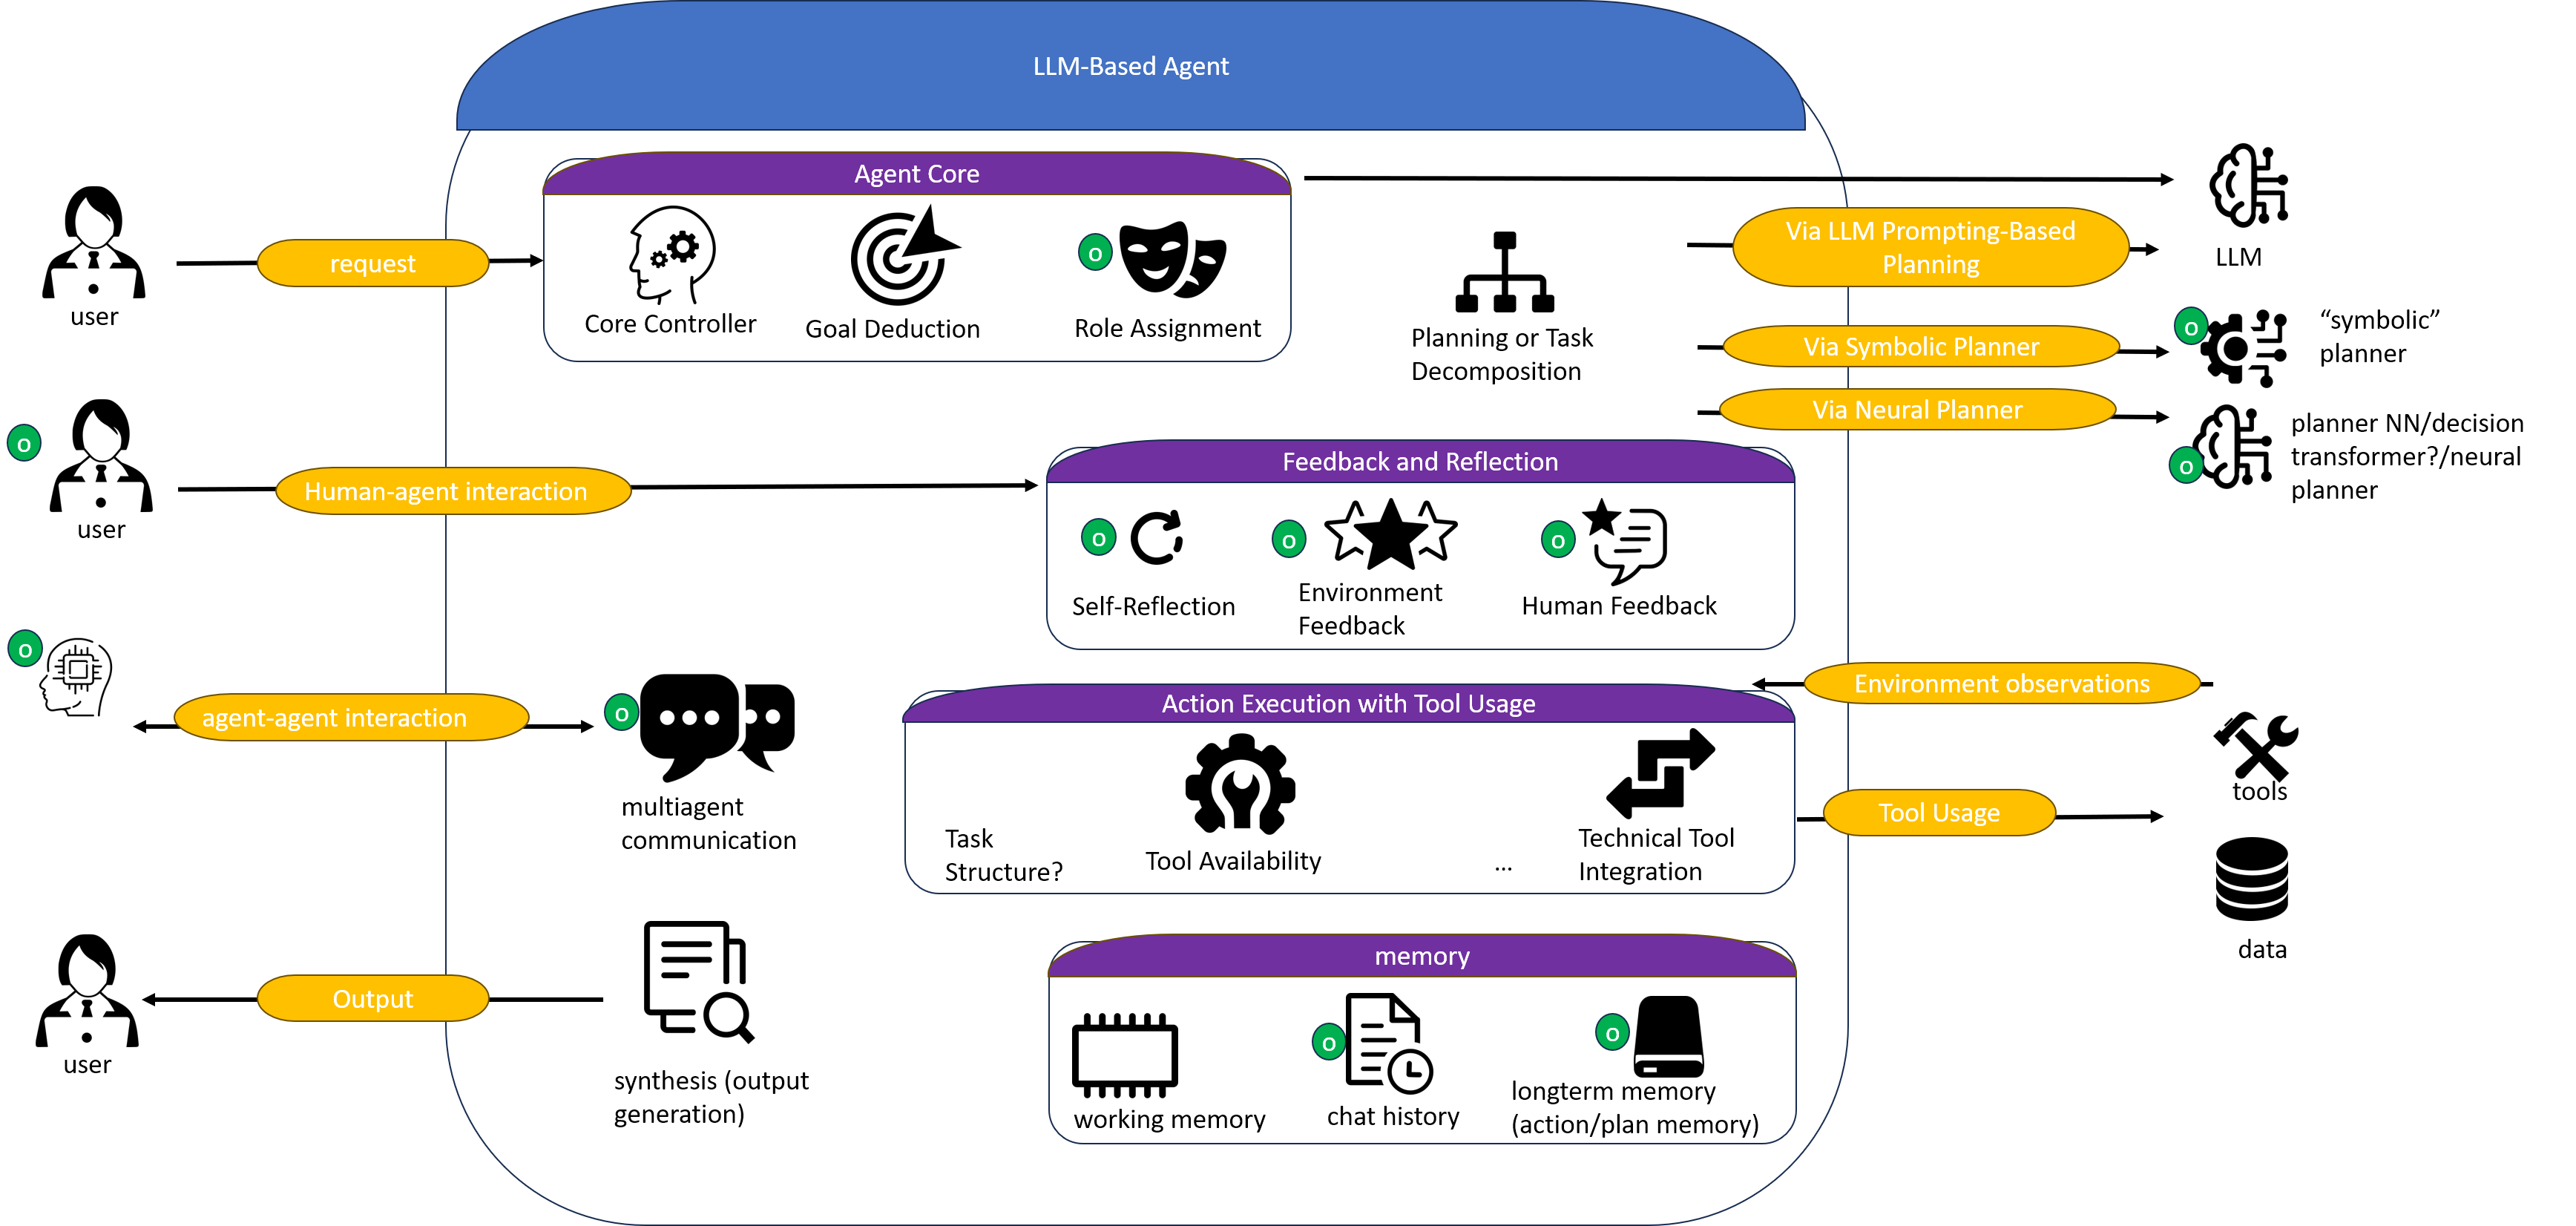
\includegraphics[width=1.0\linewidth]{LLMAgentOverview}
	\caption{PRELIMINARY PLACEHOLDER: Overview}
	\label{fig:llmagentoverview}
\end{figure}

TODO Statistics - distributions across article, 
possibly interesting statistics: preprints/reviewed, publications dates: only mention, single vs multi-agent, pure LLM vs symbolic (vs Decision transformer??/barely considered), action selection vs generation (programming)?
%timeline with number of papers? per category? reviewed publication, preprint, git repo,...
%distribution of papers...regarding techniques used
%per subject/use case/problem
%used tools
%implementation specific/programming language
%statistics: number of papers per year: per keywords eg LLM + agent, LLM+tool,...
%anecdotal??? and academic works
%input: most often text, sometimes multimodal possible
%output: text or structured data (or...?)

\subsubsection{Agent Core Controller}
DRAFT: ONLY NOTES

TODO: brief description that a program component needs to be the "core controller" that connects all the components!

Tasks of the core controller: 
-Coordination/Brain/Flow, program flow, communication between components/modules, propagate information
-storage and application/filling of LLM prompt templates/prompt library (task, additional instructions, context information, demonstrations, roles, output information like format/structure(/attributes/quality criteria/constraints) alignment techniques? (role/profiling, background information) (Role Assignment
profile/ specialist role, implicit constraints, induce behaviour)
%role alignment/generation: \cite{wang_survey_2023} three possibilities: handcrafted, LLM-generated, dataset aligned
%most approaches use some basic role attribution like, you are a helpful AI assistant, you are a household agent,...
- LLM prompting parameters and model selection (temperature, top-p, length)
- workflow of reprompting/response handling
- Input and Output/user communication handling
- memory inclusion/handling
- can add procedural knowledge
-  maybe parse to actions, execute actions (API calls etc), collect results/outputs, store, create tasks, orchestrate/execute, merge/evaluate/synthesise results
- decisions about formats, especially for prompting, intermediate results and output (e.g. YAML better than json with LLMs because of tokenization?)
- controller tasks and complexity depend on approach
- agent control operating procedures
- maybe keep track of history/encountered states (in mutliplan approaches keep track which paths already encountered)
- human communication, LLM as interface between planner and human user, task human
- possible adaption of input: Goal Deduction, user request, task(re-)formulation, What is the actual goal? , extract a planning goal from given a natural language instruction

Inspiration of operating procedures?: 

%\cite{hong_metagpt_2023} METAGPT: META PROGRAMMING FOR A MULTI-AGENT COLLABORATIVE FRAMEWORK
%"MetaGPT models a group of agents as a simulated software company"
%human workflows in LLM-based multi-agent collaboration
%Standardized Operating Procedures (SOPs) to prompt sequences, streamlined workflows, domain-expertise agents, assign roles to agents
%create intermediate structuresd output documents, similar to usual software engineering wokflow - increases success rate of target code generation
%profile definition: name, profile, goal, constraints, + provide specific context and skills
%iterative code production: Engineer role can execute unit test cases and receives test results
%ablation studies effectiveness/significance of roles

%\cite{prasad_adapt_2023} controller ADAPT:
%two options: try to execute input task directly, else call planner to decompose the task, 
%then recursively call this/controller
%communication between planner and executor, propagating information
%because of recursion: determines termination criterium

%\cite{zhou_agents_2023} Open-source Framework for Autonomous Language Agents
%not just system prompt
%instead: paradigm "controllable agents via symbolic plan" or "standard oprating procedures"(SOP)
%= graph of of states (different situations) that agent may encoutner + transition rules
%step-by-step isntruction how task should be performed
%Generation: by LLM + can be edited by user
%for deyployment agent uses SOP, behaves following the isntructions and ajusts state according to itneraction
%nedded/has ist: automated SOP pipeline to generate detailed SOP (because labour intensive): done by RAG on description of task
%can ask human for acting instad of agent
%State: modularized prompts, tools, APIs that can be used in that state
%prompts  specify task, goal, rules/constraints, demosntartirons and poutput format
%Thereby plan=SOPS and state transitions?

%role assignments/examples:
%\cite{sun_adaplanner_2023-1} basic role attribution due to environment
%ALFWorld: You are a household agent.

\FloatBarrier
\section{Plan Generation}
INITIAL FORMULATION

%Reasoning: 
%What are subgoals, what are substeps of a given task or question?
%
%Definition of reasoning
%\cite{russell_artificial_2010}
%process es of reasoning: operate on internal representations of knowledge. agents can use process of inference to derive new representaitons about the world, knwoledge-representation, deduction, logic
%
%use logic: Deuctive reasoning (deduce new information from known), inductive given facts and induce conclusion, abductive
%- we can use established methods when we have logical representation!
%common sense reasoning: informal
%monotinic vs nonmonotonic reasoning?
%
%https://doi.org/10.1145/2701413
%gary Marcus Common sense reasoning!
%\cite{davis_commonsense_2015}
%ambiguity in text/language
%taxonomic reasoning
%geographic reasoning
%temporal reasoning
%Knowledge based approaches: mathematically groudned or informal knowledge based approaches eg case based reasoning or large-scale approaches with large knowledge bases with many concepts and facts
%Web mining approaches extract common snese knowledge from web documents
%crowd sorucing approaches
%Deductive reasoning
%taxonomic and statistical reasoning on large scale knowledge bases and web mining
%what not included: reasoning by analogy, abstraction, best explanation etc

The concept of taking user input as a goal, breaking it down into tasks and solving them step by step is referred to as planning. Planning is a field in AI that deals with devising a plan of action to achieve a defined goal. It is a deliberative process by which an artificial agent reasons about, chooses and organises actions to achieve an objective \cite{ghallab_nau_traverso_2016}.   An AI planning system is a central component of an artificial agent, as outlined in \cite{wooldridge_intelligent_1995}. Typically, a factored representation is used, where the world state is represented by a collection of variables, and actions have necessary preconditions and effects related to states\cite{russell_artificial_2010}. In order to plan effectively, it is essential to have a complete and accurate domain representation and a complete, formal problem description. Algorithms to solve planning problems often include forward or backward state-space search, with the use of heuristics, Boolean satisfiability, situation calculus , constraint satisfaction and the refinement of partially ordered plans \cite{russell_artificial_2010}. 
It is not always possible or necessary to create the complete plan before starting execution. Sometimes, a partial plan is sufficient. If the environment is predictable and well modelled or if the actions have a high cost or risk or are not reversible it is advisable to create a complete plan \cite{ghallab_automated_2016}..

%In order to find a solution, e.g. forward state-space search can be applied. In this case, search begins at the initial state and tries to construct sequences of actions and checks whether a goal state can be reached. Classical search techniques like breadth-first search, depth-first search or iterative deepening can be applied. Another possibility is backward-search, meaning to begin at the goal and searching backwards until the initial state is reached. This expands only relevant states on the way to the goal and has a lower branching factor; however, less efficient heuristics are available \cite{russel2010artificial} p.376.

%receding horizon planning
% partially ordered plans => search through space of plans rather than state space (search for flaw in a plan and change)
%Reasoning: ontology, objects, semantic graphs, description logic, uncertainty: probabilistic model
%deductive: logic, inductive (like with prolog), ...

Planning is a form of deliberation. Deliberation is needed when agents need to autonomously perform in diverse environments or diverse tasks to achieve their intended objectives \cite{ghallab_automated_2016}. 
This requires a reasoning process which determines the actions to perform, how to execute them and what the result will be. Therefore, agents need some form of predictive model or simulative capabilities \cite{ghallab_automated_2016}. 
\cite{ghallab_automated_2016} describe two important principles of deliberation: hierarchical organization and continual online processing. 
The paper \cite{ghallab_automated_2016} outlines two key principles of deliberation: hierarchical organisation and continual online processing, This involves identifying intermediate goals and planning for them, refining planned actions into commands that can be executed in environment, monitoring the environment and reacting to events,and to compare predicted and observed changes, and possibly searching for recovery actions.

There are several AI planning approaches, each with different assumptions about the planning environment and planning problem (see/compare \cite{russell_artificial_2010}). Classical planning assumes a finite number of states and actions, full observability, determinism, and a static environment with a single agent. For partially observable and non-deterministic environments, contingency planning is used, where the plan contains conditional branching based on percepts. In order to reason about partially observable or unobservable environments, belief states can be utilised. In the case of unknown environments or when inaccuracies in the world model are assumed (missing incorrect variables or conditions), online replanning can be employed. This latter approach requires monitoring of action execution in order to replan if necessary. If there are multiple effectors in the world, multiagent planning can be considered.

It would be beneficial to provide a more formal definition of planning here, with an example of classical planning. A planning domain $D$ is a model representing a real-world problem, in order to enable it to be solved by AI planning systems \cite{ghallab_nau_traverso_2016}. $D$ can be based on the standard formalism of a state-transition system (see \cite{ghallab_nau_traverso_2016} p.25 and \cite{CIMATTI200335}):
\begin{itemize}%[topsep=-1em]
	%\setlength\itemsep{-0.5em}
	\item $S$: a finite set of states
	\item $A$: a finite set of actions
	\item $\gamma : S\times A \rightarrow S$: a state-transition function\\ ($\gamma(s,a)$ is  a partial function because it is only defined if action $a$ is applicable in state $s$.\\ If $\exists s': \gamma(s,a)=s'$, action $a$ is \textit{enabled} or \textit{executable}).
	\item $S\times A \rightarrow [0,\infty)$: an optional cost function\\ (It is a partial function that can be used to represent time, monetary cost or similar for a transition.)
\end{itemize}

A planning problem $P$ in the planning domain $D$ can then be defined as as a tuple $(D,I,G)$, where $I = {s_0} \in S$ is the initial state and $G \subseteq S$ is a set of goal states.

A plan is a solution to the planning problem. It describes how to get from the initial state to a goal state by using possible actions. A plan or policy can be defined as follows (\cite{KuterNau-HTNSMC}):
Let $A(s) \subseteq A$ be the set of actions $a$ applicable in state $s$. 
A plan or policy can be represented as a set of state-action pairs, with each pair describing which action to execute in which state. %DeterministicEach action in a state has only one successor state.  
In classical planning, a plan can be defined by a finite sequence of actions, such as $\langle a_1 ,a_2, a_3, ... , a_{n-1}, a_n \rangle$. 

%In general, $\pi$ can only be a solution to a planning problem $P$ if at least one goal state is reachable from the initial state by applying policy $\pi$.

Some issues can hinder the applicability of planning to practical real-world problems. One such issue is the transduction problem, which requires a significant amount of effort to create an accurate and adequate symbolic description. Furthermore, the complexity of planning must be considered. In a classical planning problem, plan-existence and plan-length are decidable, with the exemption if function symbols are used, then it is only semi-decidable \cite{ghallab_automated_2004}. The question whether there exists any plan (PlanSAT) for propositionalised problems is in complexity class PSPACE which is more difficult than NP \cite{russell_artificial_2010}. However, heuristics can be used to increase efficiency. Although classical planning seems to impose significant restrictions on assumptions about the problem, it can still be utilised in environments that do not fulfil all of these assumptions, provided that the resulting error is deemed tolerable \cite{ghallab_nau_traverso_2016}.


%Complexity
%classical planning already PSAPCE-hard??
%\cite{wooldridge_intelligent_1995}
%problem:
%already at that time to relieve? effort in planning, ideas like  the subsumption architecture Brooks 1986, 1990,1991 a,b and PENGI Chapman \&Agre 1986, where argued that many simple low-level activities don't need explicit planning

A standard encoding language for classical planning problems is PDDL (Planning Domain Definition Language). It descended from the first and highly influential major planning system and language STRIPS (Stanford Research Institute Problem Solver), and the Action Description Language (ADL).  The authors of \cite{russell_artificial_2010} (pp. 36) provide an example of an air cargo transportation planning problem in PDDL (figures \ref{fig:PDDL} and \ref{fig:PDDLSolution}).

\begin{figure}[h]
	\centering
	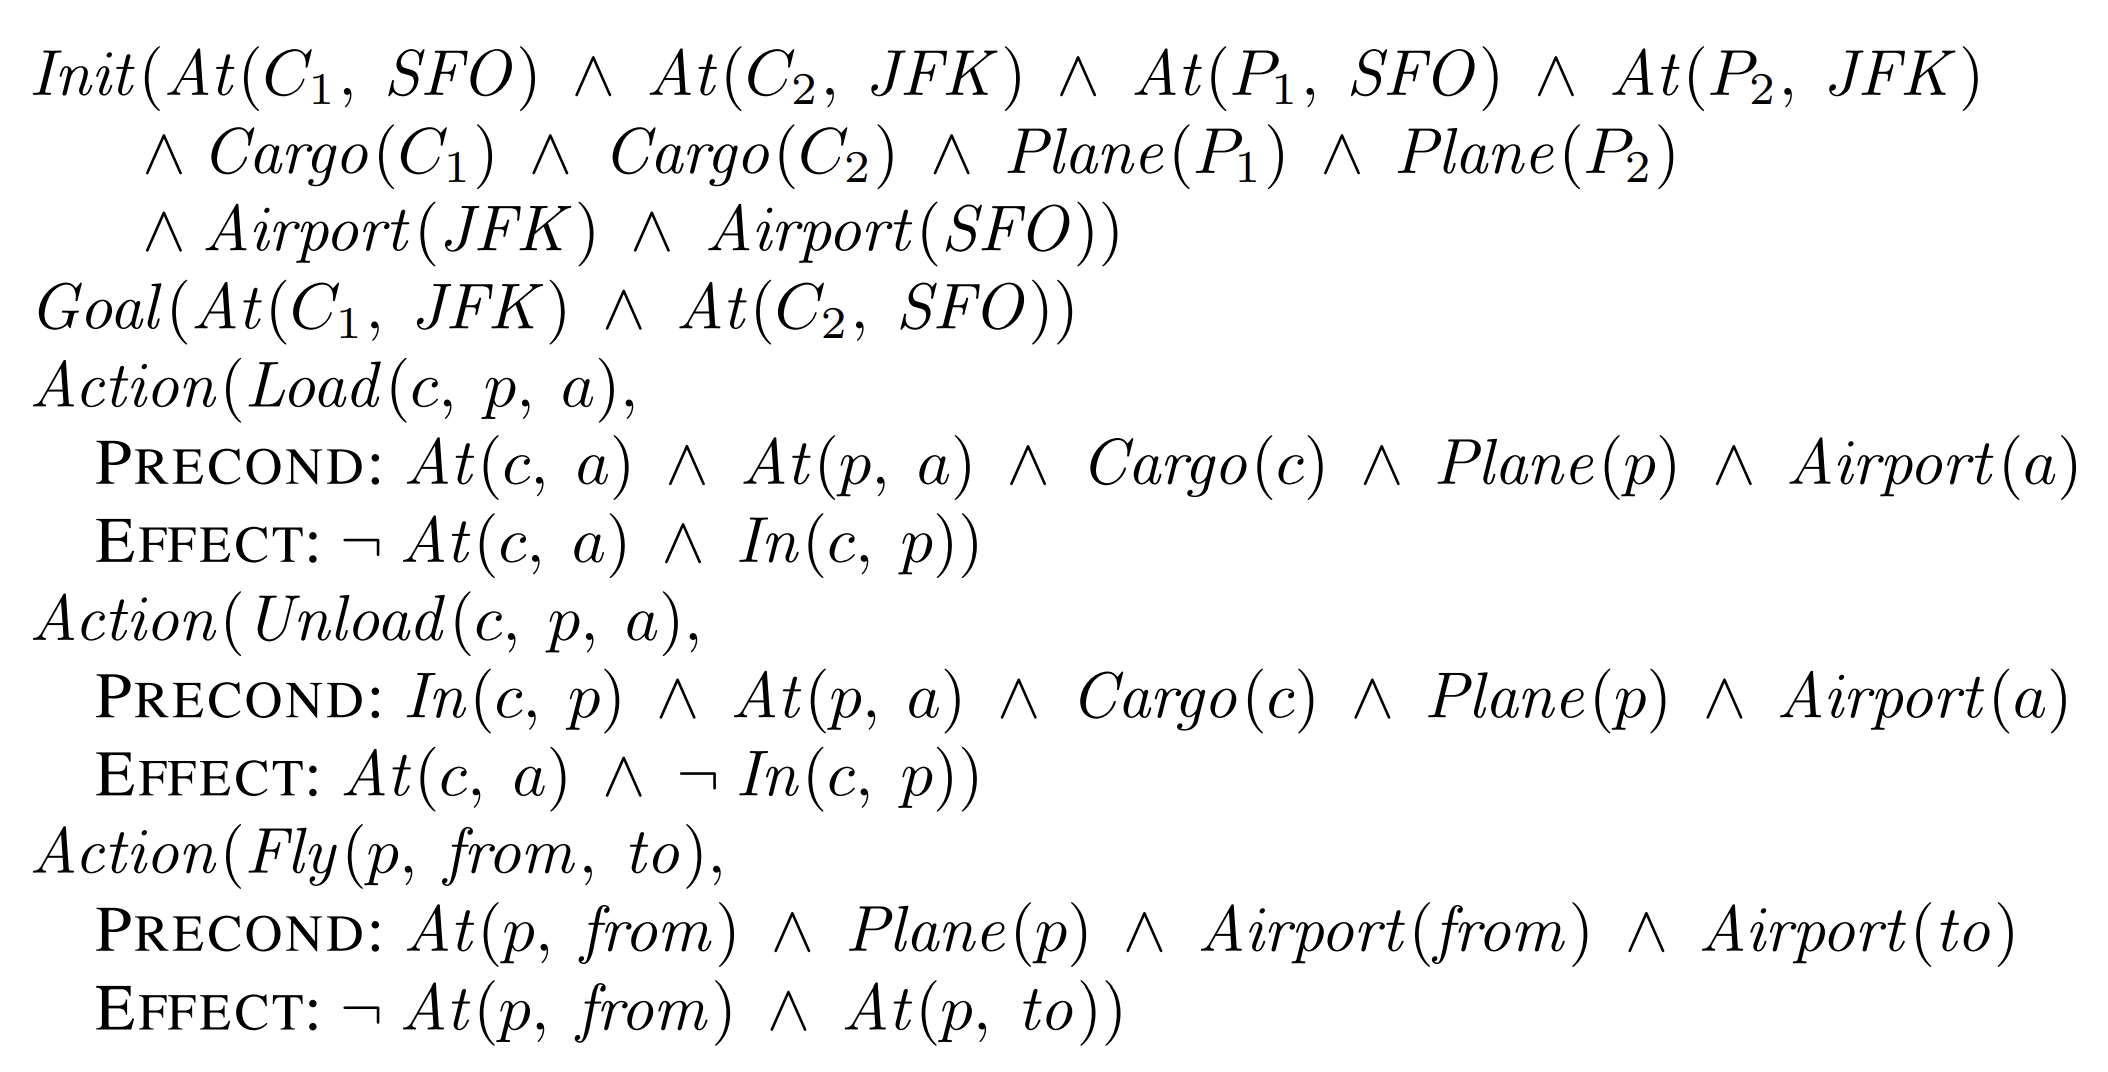
\includegraphics[width=0.6\linewidth]{RN_PDDL-AirCargo.png}
	\caption{A PDDL description (using predicates) of an air cargo transportation planning problem \cite{russell_artificial_2010}.}
	\label{fig:PDDL}
\end{figure}

\begin{figure}[h]
	\centering
	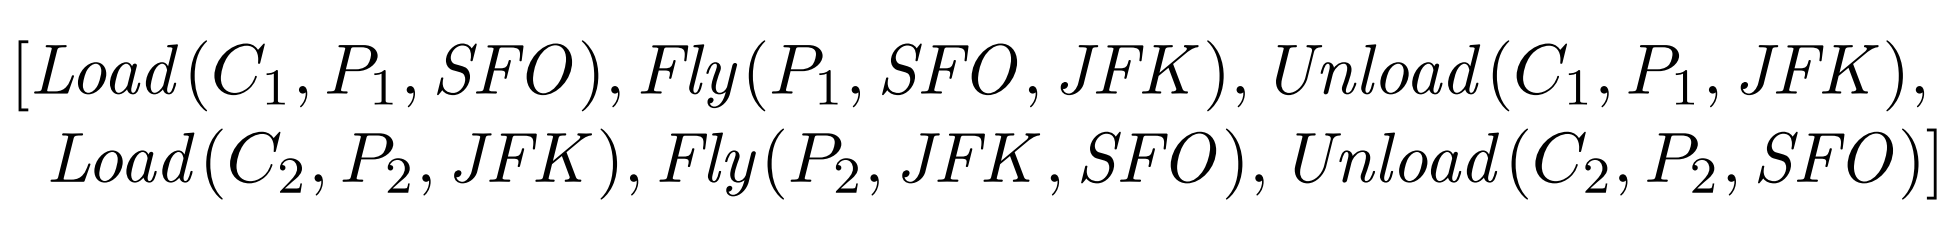
\includegraphics[width=0.5\linewidth]{RN_PDDL-Solution.png}
	\caption{A possible solution in PDDL as sequence of actions \cite{russell_artificial_2010}.}
	\label{fig:PDDLSolution}
\end{figure}


%Planning Problem Representation and Assumptions
%Structure?
%Linearity, Finiteness, Hierarchy?
%
%
%planning/classical: needs complete, accurate domain representation and complete, formal problem description
%result is a plan
%then execution separate, if tools: formulation of specific tool queries

%Planning
%Planning agents:
%Search-based problem solving agent
%hybrid logical agent (using propositional logic)
%-> planning: representation language
%classical planning: fully observable, deterministic, static environment with single agent
%factored representation, collection of variables , eg PDDL -> need to descrie initial state, availableactions, transition function(result of action application) and goal test, state conjunction of fluents, representtio of states: conjunction of fluents or set of fluents(set operations)
%Action with preconditions and effects
%Algorithms: state-space search, Boolean satisfiability, first-order logical deduction (using quantifiers), constraint satisfaction, partially ordered plans => search through space of plans rather than state space (search for flaw in a plan and change)
%Favouring?! : Hierarchical planning, hierarchical decomposition, HTN, high-level actions -> primitive actions, refinement, (set of) implementations, search for implementation from top-level action
%Why: could execute arbitrarily many actions (eg searches in database), although base actins are limitd? What actions are possible?
%building a plan library? Generalize?, reachable sets
%Percept schema: Percept actions, with precodnitions
%Contingent planning? Conditional branching based on percepts
%online replanning: execution monitoring, monitoring: action, plan, goal (levels)
%partially constructctend contingen plan -> replan
%Multiagent planning. Multieffector/multibody planning: different or even physically decoupled effectors
%multiactor, joint plan
%Belief states? Open or closed world assumption? 
%Reasoning using a general ontology? Measurements, objects, events, processes, time/time intervals, metal events and objetcs
%resoning via semantic graphs or descirtption logic
%Actually, the problem is about reasoning in uncertainty.  But no probabilistic model possible, like Bayes or relational or first-order probability model

%Planning: precondition: factored/structured representation of world states (collection of variables, eg PDDL representation)
%initial state, availableactions, transition function(result of action application) and goal test
%Algorithms: state-space search, Boolean satisfiability, first-order logical deduction (using quantifiers), constraint satisfaction, partially ordered plans, hierarchical planning, contingent planning, online replanning, multiagent planning

%\cite{russell_artificial_2010}
%key to HTN planning: construction of plan library containing known methods for implementing complex, high-level actions
%agent can also learn plans or save once cosntructed and executed plans in the plan library
%contingency planning for partially observable and nondeterministic environments
%online planning and replanning for unknown environments
%belief states: for unobservable and partially observable environments
%can also combine online planning+contingengy planning
%replanning needs execution monitoring
%replanning also needed for incorrect world model (missing precondition or effect or missing state variable)

\FloatBarrier
\subsection{Plan Generation Module}
INITIAL FORMULATION

Which methodology should be employed to generate a plan? This section outlines the various methodologies that can be employed to generate a plan. The most popular option is to utilise LLM and apply specific prompting methods developed for reasoning and planning to generate a sequence of tasks as a plan. Another option is to combine an LLM with established symbolic planners. A third option is the use of specially trained neural networks for plan generation.


\subsubsection{Pretrained LLM Inference}
INITIAL FORMULATION
%\cite{russell_artificial_2010}
%natural language= structured representation of the world (language represents objects and their relationships)

The LLM module can be used in isolation to generate a plan by decomposing a goal into subtasks. While existing approaches based on prompting are prevalent, few focus on finetuning of planning tasks. Finetuning of pretrained LLMs is not discussed here, but neural networks trained for planning are covered in section \ref{PlanningModuleNN}.

In prompting, or prompt-based learning, the objective is to provide context information to input that is deemed relevant to solve the task at hand. More formally, a template is employed to modify the original user input $x$ into a textual string prompt $x'$ with unfilled slots. The LLM is tasked with the addition of the unfilled information, resulting in the final string $\hat{x}$. This string is then used to derive the final output $y$ \cite{liu_pre-train_2021}. Two distinct types of prompt shape exist: the unfilled slot(s) may be located either in the middle of the text, which is a cloze prompt, or at the end after the entire input, which is a prefix prompt. The choice of this may depend on the model, as described in paragraph \ref{LLMBackboneModel}. 
The slots are filled by applying the function $f_{\text{fill}}(x', z)$, which searches for possible answers $z$ by calculating the probability of the filled prompts using a pre-trained language model $P(\cdot; \theta)$: $\hat{z} = \text{argmax}_{z \in Z} P(f_{\text{fill}}(x',z);\theta)$ \cite{liu_pre-train_2021}. The final choice for the slot may be made according to the maximum probability or a sampling-based approach. 
Furthermore, there can be different answer spaces Z. If Z is an unconstrained space of all tokens, then the filled-in answers z are typically used as the final outputs, as demonstrated in reference \cite{liu_pre-train_2021}. In the event that the answer space is constrained, whether in the form of an classification task or multiple-choice answers, and particularly when a pre-defined set of actions is available for selection, it is necessary to either directly map the answer to the classes or have the LLM calculate the choices' probabilities.

Prompt-based learning is particularly useful when there is little or no labelled data for specific model fine-tuning. It is also efficient because no parameters are updated and no catastrophic forgetting can occur. Prompt-based learning is also applicable in zero-shot settings, avoiding the need for defined demonstrations \cite{liu_pre-train_2021}.

However, in order to formulate effective prompts, prompt engineering is required. 
Prompt engineering can be described as the "process of creating a prompting function $f_{\text{prompt}}(x)$  that results in the most effective performance on the downstream task" \cite{liu_pre-train_2021}. 
There are specific prompt formulations for reasoning and planning tasks, such as Chain of Thought or ReAct, which will be explained in the following paragraphs.


In addition, there are general approaches to enhance prompting \cite{liu_pre-train_2021}. 
Prompt ensembling is a technique where different permutations or orders of the prompt sentences are chosen, with the masked positions altered. 
Another approach is prompt augmentation or demonstration learning. This involves the provision of a few-shot demonstration of an answered problem. 
Prompt composition is another technique where the overall prompt is defined based on composing several subprompts. 
Finally, prompt decomposition is a technique whereby complex prompts are broken down into subprompts, assuming that these are easier to answer separately. This approach is also applied in task decomposition in planning.

%dimensions: choice of pre-trained models, prompts, and tuning strategies \cite{liu_pre-train_2021}

%Prompt engineering for planning:
%\url{https://www.promptingguide.ai/techniques/react}

It is important to note that other factors can influence the efficacy of prompts, which may not be immediately apparent. For instance, \cite{jin_impact_2024} investigated the impact of reasoning step length on LLM performance and found that simply increasing the number of reasoning steps in prompts can significantly enhance LLM reasoning abilities across multiple datasets.
In few-shot settings, even the use of incorrect rationales as demonstrations is beneficial if they exhibit the requisite length of inference. In zero-shot settings, the transition from "let's think step by step" to "let's think step by step, you must think more steps" also resulted in improvements. Nevertheless, the advantage of increasing the number of steps appears to be task-dependent. The greater the complexity of the tasks, the greater the benefit of increasing the number of steps.

In addition, a code-style prompt structure can be implemented instead of relying on natural language prompts. As stated in \cite{sun_adaplanner_2023-1}, this approach reduces ambiguity and misinterpretation in the prompt, which in turn leads to a reduction in LLM hallucinations in plan generation and refinement. The authors utilise manually designed, pythonic-style coded prompts. Ablation studies demonstrated a substantial decline in performance when textual prompts were not converted to code style prompts. Code style prompts were also applied by \cite{singh_progprompt_2023} to directly prompt the LLM with program-like, pythonic code specifications of the available actions and objects in an environment. Import statements are employed to define available actions and parameters and sequences of actions operating on objects are described in function definitions. The goal of an action is still described in natural language. The approach demonstrated a notable decline in performance when natural language was employed instead of a programming language structure within the prompts.


\paragraph{LLM Backbone Model Choice}
\label{LLMBackboneModel}
INITIAL FORMULATION

%\cite{naveed_comprehensive_2023}
%
%trained in a self-supervised setting on a large corpus of text
%r fine-tuning for downstream tasks
%y significantly increasing model parameters (tens to hundreds of billions) [10] and training dataset (many GBs and TBs)
%numerous LLMs have been proposed
%"early work on LLMs, such as T5 [10] and mT5 [11] employed transfer learning until GPT-3 [6] showed LLMs are zero-shot transferable to downstream tasks without fine-tuning."
%transformer archtiectures"Encoder Decoder: This architecture processes inputs through the encoder and passes the intermediate representation to the decoder to generate the output."
%Causal Decoder: e predicted token depends only on the previous time steps
%Prefix Decoder: attention calculation is not strictly dependent on the past information and the attention is bidirectional
%Mixture-of-Experts: parallel independent experts and a router to route tokens to experts
%T5 [10]: An encoder-decoder model employing a unified textto-text training
%GPT-3, 175B parameters
%PaLM [15]: A causal decoder
%PaLM-2 [123]: A smaller multi-lingual variant of PaLM
%LLaMA [127, 21]: A set of decoder-only language models varying from 7B to 70B parameters.
%LLaMA-2 [21]: This work is more focused on fine-tuning a safer and better LLaMA-2-Chat model for dialogue generation
%CodeGen [130]: CodeGen has similar architecture to PaLM,trained on both natural language and programming language data sequentially
%CodeT5 [136], with shallow encoder and deep decoder, trained in multiple stages initially unimodal data (code) and later bimodal data (text-code pairs)
%Alpaca, Vicuna: Llama instruction tuned

The question of which LLM to choose as the backbone for an agent when the LLM is used for plan generation must be addressed. Prior to selecting a specific model, it is advisable to select the general agent architecture, which should be the most suitable composition for the task at hand. Once the general architecture has been selected, the specific model can be chosen based on the task and the agent architecture.

There are different LLM architectures, and the fundamental differences between them are briefly explained in the following paragraphs.

\begin{itemize}
	\item \textbf{Encoder-decoder} architectures (\textbf{Seq2seq} models) have two transformer block stacks, an encoder and a decoder. In the encoder, input is encoded into latent representations using multi-head self-attention layers. At the output, cross-attention? is used to generate the target output sequence. Encoder decoders are particularly useful for tasks requiring contextual understanding in conjunction with generation. Well known examples are T5 and BART.
	\item In the \textbf{causal decoder} architecture (also \textbf{autoregressive} language models) there is no encoder, only a decoder stack with a unidirectional attention mask. Therefore, each input token only attends to the previous tokens, including itself, and the predicted tokens only depend on the previous ones. The goal of pre-training is to predict the next word by estimating the probability distribution of a text given the previous tokens. Causal decoders are strong in text generation tasks. The most prominent examples are the GPT series models.
	\item The architecture of the \textbf{prefix decoder} is similar to that of the causal decoder, but the masking mechanism allows bidirectional attention over input tokens. The output tokens are also generated autoregressively.
	\item The \textbf{encoder-only} architecture (\textbf{autoencoder}) is used where only the contextual encoding of the input sequence is relevant, and not the autoregressive generation. Instead, the output is a sequence of embeddings. The goal of pre-training is to correct corrupted data, where input parts are masked and the model has to fill in the blanks. A prominent example is BERT and all its successors.
	\item The \textbf{Mixture-of-Experts} (MoE) approach can be applied to any architecture. Here, the dense feedforward parts are replaced by an MoE layer containing different 'experts' (neural networks) and a router or gate network that decides which expert to route which token to. This allows sparser computation in training and inference, because instead of activating the whole dense layer per token, only the subset of selected experts is activated.
\end{itemize}


%especially where pre-trained models are not fine-tuned on specific tasked, but textual prompts are used to reformulate the tasks to look more similar to the tasks the LLM was originally trained with \cite{liu_pre-train_2021}. 

It is considered critical to adapt the prompting method to the architecture of the chosen model, as the training objective is important in determining the applicability of the modes to particular prompting tasks \cite{liu_pre-train_2021}. For example, prefix prompts should be used with autoregressive models, whereas cloze prompts could be used with bidirectional architectures.

In summary, it may be advisable to first work out the most probably suitable LLM architecture for the task and the overall agent architecture. For example, if the LLM is to do all the plan generation, perhaps a different model needs to be chosen than if the model is to translate textual information into PDDL and call an external planner. If it is possible to compare several models, ablation studies of the overall agent architecture with different LLM models can be conducted to find the most appropriate LLM.


This section includes evaluations that compared multiple LLMs on planning or very similar tasks. The following provides a brief overview of the evaluation studies. The results and comparisons are presented in a concise summary in a table, which facilitates the identification of differences and enables the assessment of the suitability of different models as agent backbones, particularly for plan generation. [[Furthermore, if the approaches examined in this work included comparisons of diverse LLMs as backbone models, the results are also included in the table. The aforementioned approaches are described in their respective sections and not replicated here.]]

\begin{figure}[h]
	\centering
	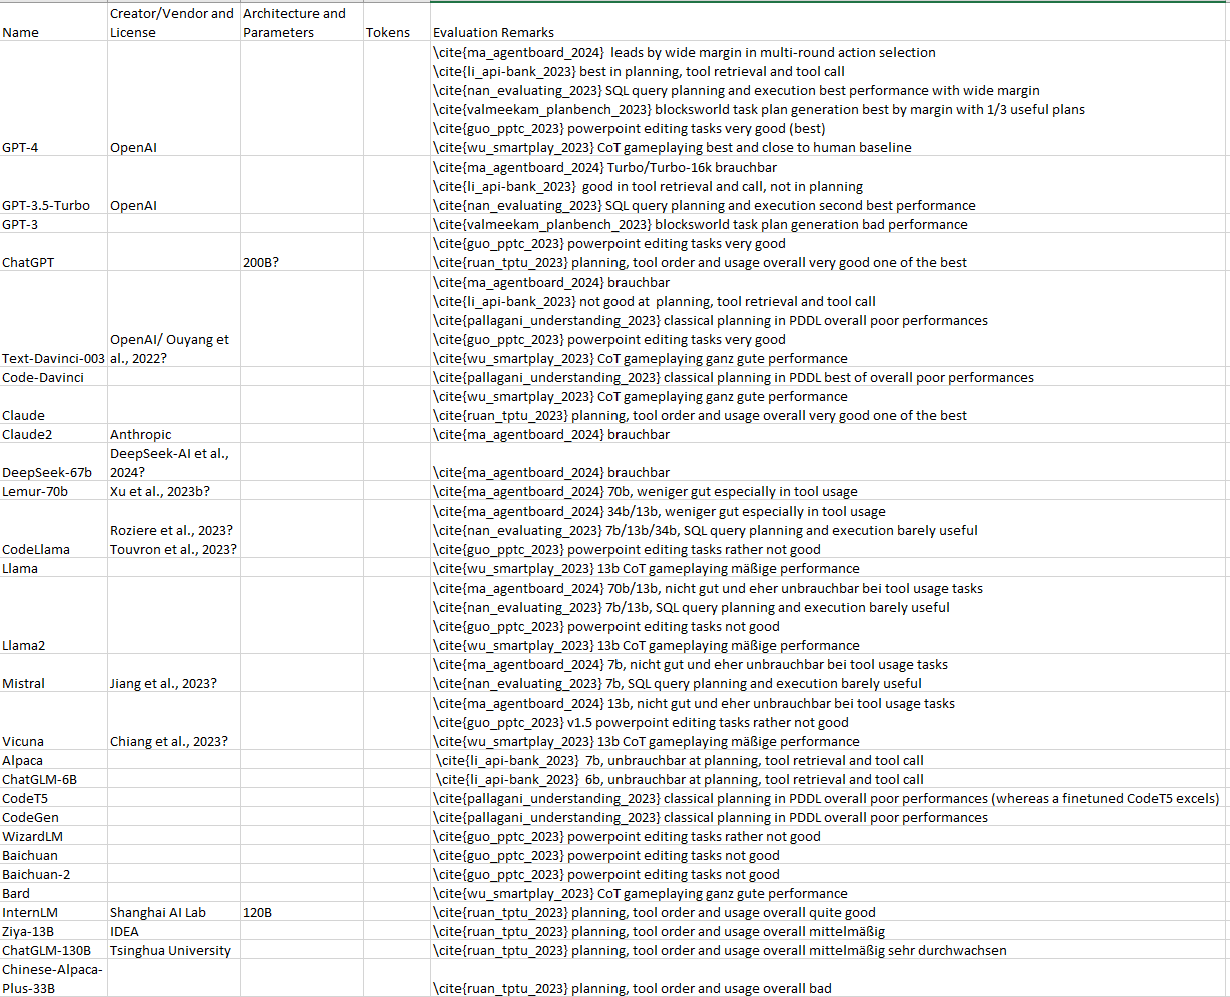
\includegraphics[width=1.0\linewidth]{LLM-Evaluation}
	\caption{PRELIMINARY DRAFT - Will be colour-coded to identify best potential, LLM comparison summary of different benchmark articles overview}
	\label{fig:llm-evaluation}
\end{figure}

%Vicuna: fine-tuned Llama on user-shared conversations from ShareGPT, fine-tuning as chatbot
%Aleph Alpha??:
%Aleph Alpha Luminous Explore: generates representations (embeddings9 of text
%luminous-base: finetuned. Kein RLHF
%GPT-3.5, decoder-only transformer, 175 billion parameters (3:175 million), RLHF finetuning (supervised data with human preferences: train network on that dataset, use the trained network to findetune GPT-3.5)
%GPT-4 RLHF, multimodal, decoder-only transformer?
%Llama-2 (Llama-2 Chat: finetuned, RLHF) standard transformer architectrure??? based on GPT???
%Claude-2
%Flan-T5 FLAN-T5 was released in the paper Scaling Instruction-Finetuned Language Models - it is an enhanced version of T5 that has been finetuned in a mixture of tasks. Text-to-Text Transfer Transformer + Finetuning large lagnuage models
%Mixtral?? sparse mixture of experts (MoE), several virtual experts, for every prompt, pool of experts is pickedfinetuned language versions, finetuned instruct version

\begin{itemize}
	\item \cite{ma_agentboard_2024} evaluated the performance of various LLM models across a range of tasks in four distinct partially observable, multi-round environments of embodied AI, games, web tasks and tool usage. The LLM's task was to determine the particular best subsequent action.
	\item In order to evaluate LLM API tool call abilities, \cite{li_api-bank_2023} conducted a study in three distinct settings: tool call based on user queries, tool calls + tool retrieval (search), tool call + retrieval + planning. Only GPT-4 could succeed in the last category.
	\item In their study, \cite{nan_evaluating_2023} evaluated the reasoning and action of LLM agents in answering database questions. To do so, the LLM agents were required to interact with an SQL interpreter and generate multiple queries. The study employed two different settings. In the sequential setting, the LLM agents acted in a linear sequence of interaction planning, tool employment, and information synthesis. In the iterative setting, the agents alternated between interaction planning and tool employment.
	\item \cite{pallagani_understanding_2023} tried to use LLM reasoning capabilities on plain PDDL domain and problem files of six classical planing problems to devise a plan i.e. find a sequence of actions to achieve the defined goal. Using the plain files with prompting and without finetuning resulted in overall poor performance, whereas LLMs pretrained on code showed slightly better performance and argue that maybe encoder-decoder architectures might be better than decoder only for such tasks
	\item In their study, \cite{pallagani_understanding_2023} sought to utilise the reasoning capabilities of LLM on  plain PDDL domain and problem files of six classical planning problems. The LLM objective was to devise a plan, namely a sequence of actions that would achieve the defined goal. They tested an approach only based on prompting and a finetuning approach. Solely relying on prompting resulted in overall poor performance. LLMs pretrained on code demonstrated slightly better performance. Furthermore, the authors argue that encoder-decoder architectures may be more suitable for such tasks than decoder-only architectures.
	\item The authors of \cite{valmeekam_planning_2023} investigated the claims that LLMs have the ability to reason, particularly in terms of planning and sequential decision-making. This involves creating a policy that leads, by executing it, to a goal state. The article examines the plan generation capabilities of LLMs in three different settings and on simple blocksworld tasks. In the setting where LLMs were required to autonomously generate and validate simple plans on blocksworld, they demonstrated very limited planning abilities, with only 3\% of the plans being executable without error and reaching the goal. This was improved in a later repeated experiment with GPT-4, which outperformed all other models and reached more than 34\% in plan generation. In a further setting, LLMs were required to develop a plan draft as a heuristic, which was then provided to the local search planner LPG [9]. This approach utilised the flawed generated plan as a seed and could iteratively repair the flaws to identify a correct plan. All the plans generated by this approach were  valid. In the final setting, the LLMs draft plan was presented to a human, who could utilise it as inspiration. A greater proportion of individuals who were provided with plan suggestions were able to generate a correct plan than those who were not.
	\item \cite{guo_pptc_2023} created a PowerPoint task completion benchmark with multiturn, multi-model instructions to test the ability of LLM systems to create and edit PowerPoint files. The primary challenges and sources of error for the LLMs were the accumulation of errors during the multi-turn session, the lengthy processing of long PPT templates, and the difficulty of multi-modality perception. In general, the results indicated that open-source LLMs exhibited lower performance than closed-source models, and smaller models demonstrated inferior performance compared to larger models. Additionally, it was found that CoT \ref{} and ToT \ref{}, in conjunction with access to the dialogue history, exhibited a slight improvement in the performance of GPT-4, while ToT did not outperform the relatively simple CoT, despite requiring a significantly greater number of tokens.
	\item \cite{wu_smartplay_2023} tested the ability of LLM to decide the next action in six different games, including Rock-Paper-Scissors, Tower of Hanoi and Minecraft. The researchers employed a direct prompting approach, initially querying “What is the next action to take, let’s think step by step.”. They also provided a manual, the history, and the current observation as context. Subsequently, they queried “Choose the best executable action from the list of all actions. Write the exact chosen action." to map the chosen action to one of the environment actions.
	\item In the study \cite{ruan_tptu_2023}, the authors compared LLM performance on task planning and tool usage in tasks such as SQL query formulation and Python code generation with 12 available tools. Two distinct approaches were tested: One approach is that of the one-step agent, which instead of attempting to solve the entire problem in one go, breaks it down into a sequence of subtasks and generates a plan in an offline manner. By contrast, the sequential agent method involves resolving the current subtasks and generating the next task in an iterative manner. Furthermore, they examined different partial tool usage capabilities, including tool order planning, subtask description generation and the planning of tool and subtask pairs.
\end{itemize}



%TODO ist this relevant? not yet added
%\cite{sun_adaplanner_2023-1}
%GPT3.5 gpt-3.5-turbo underperforms eg cpompared to predecessor text-davinci-002, authoras observed noticeable hallucination, assume smaller model prone to hallucination +  omptimization for human conversation impinges on other tasks like code generation and reasoning 

%TODO specific approaches 
%\cite{singh_progprompt_2023} PROGPROMPT best performing backbone LLMs: GPT-3 variants, Davinci- 003 and Codex

\paragraph{Prompt Augmentation for Reasoning}

TODO: INTRO

if giving in prompt more context information in form of demonstrations: prompt-based learning ... 
In prompt-based learning, the provision of additional contextual information in the form of demonstrations is


\subparagraph{Zero-Shot Planning Prompts}
INITIAL FORMULATION

Analogous to a standard zero-shot prompt, the zero-shot planning prompt merely contains the task with the directive to create an answer or a plan, without any additional demonstrations of, for example, an exemplary plan with subtasks. In zero-shot planning, no task-specific training data is required, thus avoiding the manual effort of crafting demonstrations. Conversely, there is no possibility of conditioning the LLM on how the intermediate steps, for example in planning, should ideally look like or if the output should exhibit a certain structure demonstrated by examples. Consequently, in zero-shot, the model is more reliant on pretraining data, as no new data is incorporated into the prompt for in-context learning. Zero-shot approaches are adaptable to a wide range of tasks, as no task-specific knowledge is required, and they consume fewer tokens in inference than few-shot prompts, as only the task and some directives are prompted.

%zero-shot , think step by step: \cite{kojima_large_2023} 29.01.2023
%faithful reasoning: \cite{creswell_faithful_2022}, requires finetuing of two models


A specific prompt to enhance reasoning and planning capabilities without the need for demonstrations is zero-shot chain of thought (CoT), introduced by \cite{kojima_large_2023}. The objective is to decompose the task into a series of explicit intermediate reasoning steps. 
This is essentially almost equal to a zero-shot prompting query to an LLM. The prompt template is just  the addition of the phrase "Let's think step by step" to the original question. This results in the generation of an intermediate output comprising a series of reasoning steps. Subsequently, the LLM is queried a second time with the initial input prompt and the corresponding output and with "Therefore, the answer is," accompanied by optional information such as the desired output format. 
The authors demonstrated that the incorporation of these sentences resulted in a notable enhancement in the zero-shot LLM accuracy performance on a range of benchmark reasoning tasks, utilising GPT-3, InstructGPT and PaLM. Furthermore, the listing of intermediate steps  seems to provide insight into the reasoning process. 
It was demonstrated that Zero-Shot-CoT was unable to outperform Few-shot-CoT when the latter was provided with carefully crafted and task-specific step-by-step examples. However, Few-shot-CoT necessitates human engineering and is highly sensitive to examples. %Consequently, few-shot performance is negatively affected by the use of unmatched examples.
The results also demonstrated that CoT was not effective when applied to models with a small size. CoT proved effective on GPT-3 and InstructGPT, with a model size of 170B, and on PaLM, with a model size of 540B. The remaining tested models, all having less than 13 billion parameters (with the exception of PALM, which had 63 billion parameters) were found to be ineffective when using CoT. The authors of \cite{zhang_igniting_2023} complement that  CoT is effective for LLMs with more than 20 billion parameters and if the LLM encompasses pretraining knowledge relating to the task.


\begin{figure}[h]
		\centering
		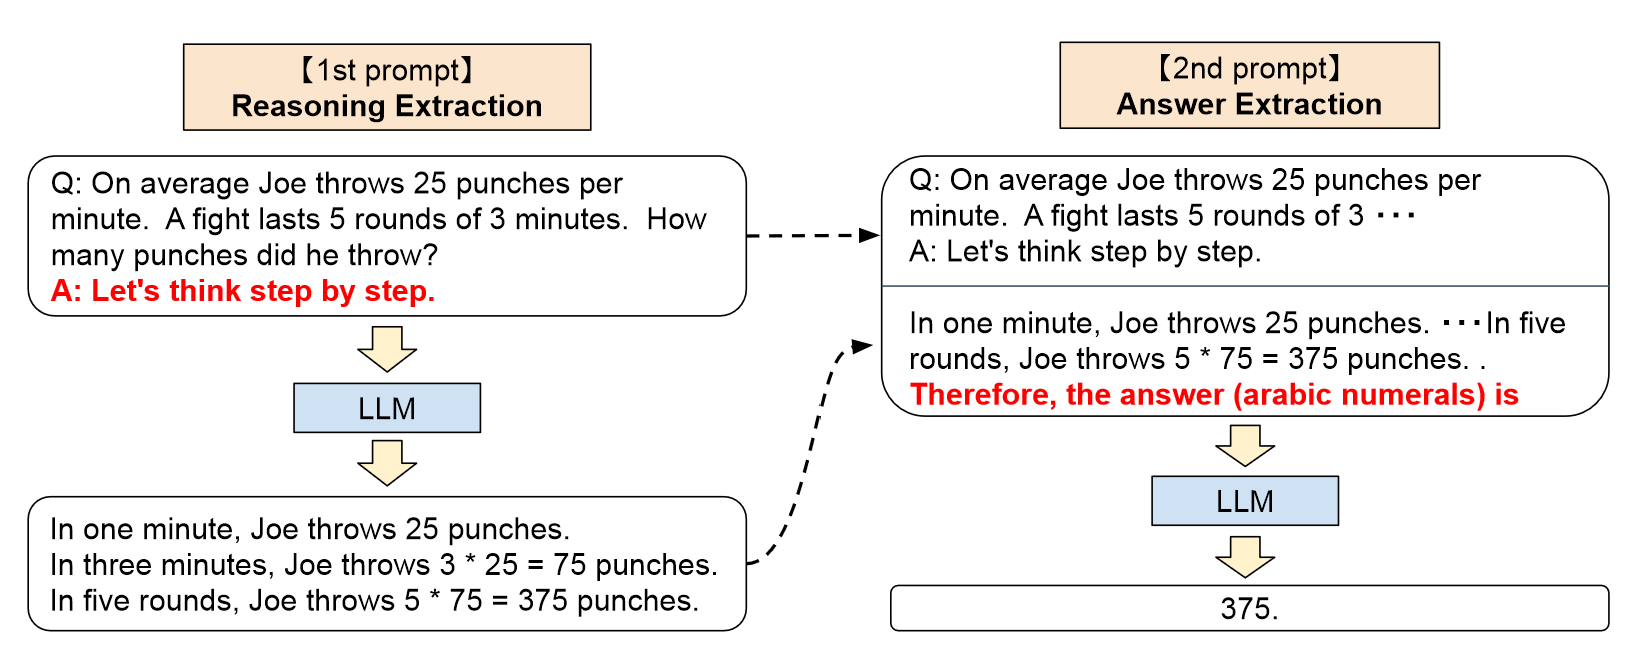
\includegraphics[width=0.7\linewidth]{ZeroShotCoT.png}
		\caption{Example of a zero-shot CoT prompt \cite{kojima_large_2023}}
		\label{fig:zeroshotcot}
\end{figure}



In their approach, \cite{wang_plan-and-solve_2023}, the authors adapted the concept of CoT and divided the reasoning process into two stages: the generation of the steps of a plan and the subsequent execution of the steps. In order to achieve this, the following sentence was included in the prompt: "Let's first understand the problem an devise a plan to solve the problem. Then, let's carry out the plan and solve the problem step by step." The second step is analogous to the CoT approach, whereby the final answer is prompted for, for instance, in the context of mathematical reasoning: “Therefore, the answer (arabic numerals) is”.  It is also possible to extend the prompt instructions as follows: “extract relevant variables and their corresponding numerals” and “calculate intermediate results (pay attention to calculation and commonsense)”.  The results of the study indicate that Plan\&Solve prompting outperforms Zero-shot CoT across a range of reasoning test problems. This approach can be extended with self-consistency (SC) \ref{}, to reduce randomness by generating multiple sample results and selecting the majority vote. According to the authors, applying SC significantly enhances performance.



\subparagraph{Few-Shot Planning Prompts}
%in-context learning/demonstrations, performance dependent on selected demnstrations
INITIAL FORMULATION

The concept of few-shot learning is to enhance in-context learning by providing new data that is not included in the pre-training data of the model. This is achieved without the need to directly train or finetune the model by changing the weights. In-context learning can be applied on a task-by-task basis, as the demonstrations can be tailored to specific tasks. This necessitates either the manual creation of suitable examples or an approach of automatically generating those examples. Few-shot prompting requires a greater number of tokens, as the examples and the original task are appended and then prompted to the model. The provision of numerous demonstrations may consume a significant proportion of the context window size and may also result in an increase in inference time. Consequently, it is not always possible to utilise this approach when extensive demonstrations or a large number of examples are required. 

%GENERAL NOTES:
%Disadvantages: Because prompts are the only method that provide the task specification, heavy engineering is necessary to achieve high accuracy. In particular in the in-context learning setting, providing many answered prompts can be slow at test time, and thus cannot easily use large training datasets." \cite{liu_pre-train_2021}
%-prompt augmentation/demonstration learnng: demonstartions of answered prompts, few-shot demonstrations (questions: how to choose the most effective samples and how to order them?)

\cite{zhao_calibrate_2021} conducted research with the objective of improving the few-shot performance of language models. The study demonstrated that three components of a prompt, format, set of training examples and permutation (ordering) of the examples exert a significant influence on the accuracy of GPT-3 and GPT-2. The research identified three biases that can negatively influence performance. The majority label bias implies a greater probability of predicting responses that appear frequently within the provided examples. The recency bias implies a greater probability of predicting responses that are similar to those that appear at the end of the prompt. Furthermore, the common token bias implies a higher probability of predicting answers that are frequent in the pre-training data. The authors employed content-free test prompts to measure the possible bias and subsequently applied a weight matrix and a bias vector to calibrate the output distribution of the original probabilities. This resulted in a consistently improved and stabilised accuracy.

In \cite{wei_chain--thought_2022}  the authors introduced the concept of chain of thought prompting and demonstrated its efficacy in enhancing the ability of large language models (LLMs) to perform complex reasoning tasks. The authors describe chain of thought as a "series of intermediate natural language reasoning steps that lead to the final output". This approach is inspired by the human thought process of tackling complex reasoning tasks as a multi-step problem. In practice, each query is enhanced with a few examples of chain of thought intermediate reasoning steps for similar tasks and responses.
\begin{figure}[h]
	\centering
	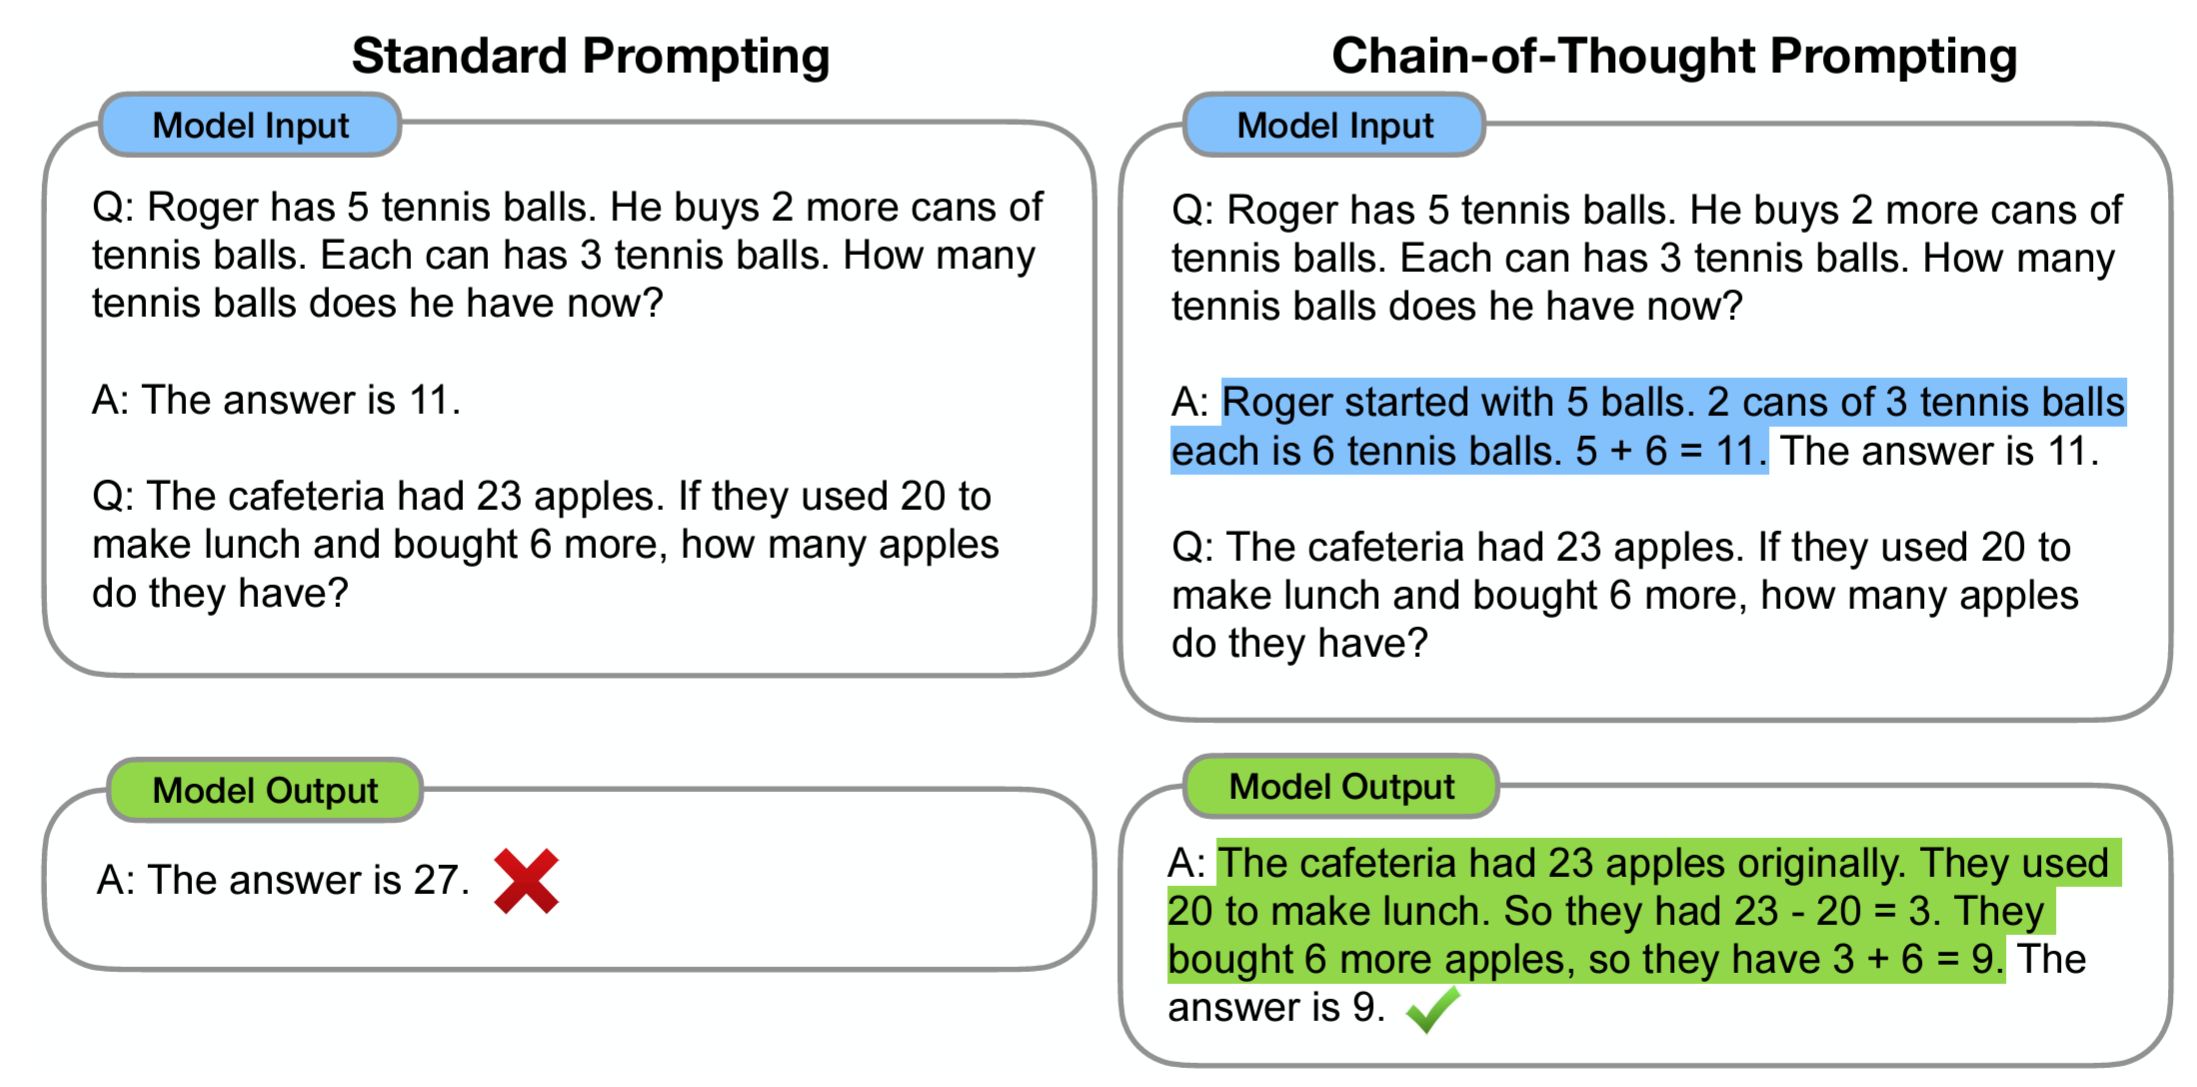
\includegraphics[width=0.7\linewidth]{CoTExample}
	\caption{Chain-of-thought prompting example\cite{wei_chain--thought_2022}}
	\label{fig:cotexample}
\end{figure}
It should be noted that CoT reasoning only increased performance with large model scales. For instance, for arithmetic reasoning and symbolic reasoning, the required model parameter size is at least 100B. This makes the application of CoT expensive. Furthermore, they found that in smaller models, the production of illogical chains of thought can even lead to lower performance than standard prompting.

In order to enhance the efficacy of CoT, it is beneficial to ensure that the demonstrations align with the actual task. Accordingly, \cite{song_llm-planner_2023} employ task-specific in-context example retrieval. Prior to utilising this approach, it is necessary to have a training set comprising pairs of instructions and examples. The authors utilise a pre-trained BERT-base model to assess the pairwise similarity between the test example and training examples, employing the Euclidean distance between the BERT embeddings of the corresponding instructions. Subsequently, the K most similar examples can be selected for the purpose of augmenting the prompt.


TOTO: ADD Least-to-most prompting 
https://doi.org/10.48550/arXiv.2205.10625 Poster presentation at ICLR 2023 without link/doi??



%TODO REMOVED FROM ARTICLE; BECAUSE RATHER STANDARD HIERARCHCIAL DECOMPOSITION; NOT LLM PLANNING
%HIERARCHICAL DECOMPOSITION BUT VERY BAD ARTICLE
%\cite{zhen_robot_2023} 08.06.2023 Robot Task Planning Based on Large Language Model Representing Knowledge with Directed Graph Structures
%Think\_Net\_Prompt template: combine human expertise with LLM, represent structured professional knowledge, eas to configure, recursively layer tasks,d ecopose tasks layer by layer
%Method to "rogressively decompose tasks and generate a task tree to reduce the planning volume for each task"
%unstructured robotic environments
%Robot task and action planning problem
%LLM need to "decompose high-level commands into a sequence of usable low-level skills"
%"there hasn't been serious consideration for a general method of providing more complex structured professional knowledge for the semantic understanding capabilities of LLM"
%the more complex the task description the worse the quality of results of prompting methods
%direct graph structure that describes the isntructions et
%JSON input format
%For main task word, generate root node of tree, generate subtask sequence, repeat to generate subtaks until leaf nodes are reched, always check if it is a valid task word before expanding
%await a fixed json input format and given output format in json format as task sequence. demonstrations of inputs and outputs
%awaits lot of information   task name and additional information, possible subtasks and their description and parameters
%LLm can then decide which to choose
%ME: not clear why LLM is needed, is just a hierarchical deocmposition??!! not a good paper, very shallow experiments and anylsis, value of this contribution absolutely not cleear


%TODO ONLY ADD WHEN TOO MUCH TIME; NOT QUITE RELEVANT; MANY (IMPLICIT) ASSUMPTIONS
%NOT PLANNING, JUST DIFFERENCE IN PROMPT...
%\cite{tang_towards_2023} 04.09.2023 Towards CausalGPT: A Multi-Agent Approach for Faithful Knowledge Reasoning via Promoting Causal Consistency in LLMs
%framework to increase faithfulness and causality for knowledge-based reasoning
%multiple agents: reasoners and an evaluator
%reasoners: provide solution, human-lke causality
%evaluator: solution deducible from non-causal perspective? solution holds when challenged by counterfactual candidate?
%"intelligent agents with different roles and weights engage in a reasoning-and-consensus process to accommodate potential errors"
%causal-consistency reasoning framework, named CaCo-CoT
%resoners: prerequisite steps sequentially, i.e., terms explanation, subquestion decomposition, rationale before arriving at an answerm "1) explaining necessary concepts or principles and 2) breaking down the problem into a list of subquestions"
%until consensus is reached
%nowledge-based reasoning (KR) problems, problems require background knowledge. BUT here: usejust LLMs with over 100B parameters and assume they have necessary background knowledge
%agents: prompting an LLM with in-context learning capability
%prompt template involves a sequence of {concept explanation, subquestion decomposition, rationale generation, answer synthesization}, reasoner reasons in causal style
%evaluator: asees faithfulness of solutions (solution = including all reasoning steps), inspect/evaluate solution +  replace answer in solution and then search for contradictions
%Several reasoners generate solutions with answers. If answer reaches  bigger than threshold consensus amongst reasoner agent, evaluator examines solution. Otherwise evaluate solutions of top n answers
%GPT-3.5-turbo and Claude for agents and
%GPT-4 used to generate solutions to questions and this is provided as context



Demonstrations can also contain cues to actively request follow-up questions and gather more information within the stepwise reasoning process, thereby enhancing performance on compositional reasoning. 
In the study \cite{press_measuring_2023}, the researchers were concerned with the question of how to measure and increase the ability of compositional reasoning. This means that, in order to reach an overall solution, the answers to the subproblems must be composed. They found that an increased model size alone does not lead to an improvement in the ability to perform compositional reasoning. Conversely, it has been demonstrated that elicitive prompting, such as CoT, enhances the capacity to perform compositional reasoning by encouraging explicit reasoning. The authors propose the self-ask approach to enhance CoT, which involves prompting the LLM to ask self-questions. In order to achieve this, they include within the demonstrations an initial question, followed by an intermediate question and, where appropriate, a series of follow-up questions and corresponding answers. It is possible that intermediate questions could be answered by the LLM itself, but it is also possible that a tool such as a search engine could be employed.
\begin{verbatim}
	Question: Who lived longer, Theodor Haecker or Harry Vaughan Watkins? 
	Are follow up questions needed here: Yes. Follow up: How old was Theodor Haecker when he died? Intermediate answer: Theodor Haecker was 65 years old when he died. 
	Follow up: How old was Harry Vaughan Watkins when he died? Intermediate answer: Harry Vaughan Watkins was 69 years old when he died. 
	So the final answer is: Harry Vaughan Watkins
\end{verbatim}

The concept of a chain of thought can be expanded to encompass not only valid reasoning demonstrations, but also invalid ones. 
In \cite{chia_contrastive_2023}, the authors introduced the concept of Contrastive Chain-of-Thought Prompting, which involves providing examples of valid and invalid reasoning, the latter with the idea to demonstrate which mistakes to avoid. To obviate the necessity of manually constructing negative examples, contrastive demonstrations are constructed automatically from existing valid reasoning chains. Invalid examples can be constructed by invalidating valid reasoning, for example by destroying coherence by changing the ordering of steps, or creating object and language incoherence by shuffling object or word positions or introducing irrelevant objects.
In their experiments with GPT-3.5-Turbo, the provision of positive and negative demonstrations led to a significant improvement in CoT. The approach is even more effective when combined with self-consistency (see \ref{}).

\begin{verbatim}
	Question : <demonstration question>
	Explanation: <correct demonstration explanation>
	Wrong Explanation: <incorrect demonstration explanation>
	Question: <actual question>
\end{verbatim}

It is possible to enhance the prompts in simple ways, thus adding specific reasoning capabilities. An illustrative example is the work of \cite{zhang_large_2024}, which demonstrates that a simple prompt can be used to instruct an LLM to conduct a mathematical proof of contradiction. 
An explanation of the proof is provided in the prompt, which is followed by demonstrations of some applications of the proof.
\begin{verbatim}
	<Instruction> Proof by contradiction in logic and mathematics is a proof that determines the truth of a statement by assuming the proposition is false, then working to show its falsity until the result of that assumption is a contradiction.</Instruction>
\end{verbatim}


A limitation of few-shot planning prompts is their lack of generalizability, as explained in\cite{gao_strategyllm_2024}. Demonstrations are made of solutions specific to a given task and do not easily apply to other cases. Furthermore, if several demonstrations are included in a prompt and employ different solution strategies to solve the same task, this can "confuse" the LLM. Consequently, the objective is to derive general strategies from task examples and to "construct generalizable and consistent few-shot prompts for various tasks automatically".
To identify strategies for a task, the authors employ LLMs in four distinct roles. The role of strategy generator formulates a pool of task-solving strategies based on task examples: 
\begin{verbatim}
	Task: 
	{task definition} 
	
	Some examples of the task are as follows: 
	{task examples} 
	
	Let’s understand the task and write a strategy that consists of a sequence of subtasks to solve the task. For writing, you must satisfy the following requirements: 
	- Include all necessary subtasks. 
	- All subtasks are easy to solve. 
	- Subtasks are in an appropriate order. 
	- Do not include specific information in the examples. 
	- Make sure the strategy is general and concise. The result must be a numbered list in the following format: 
	1. First subtask 
	2. Second subtask
\end{verbatim}
The strategy executor applies the strategies to task examples, obtains results, and computes the respective accuracies. In the event that an insufficient number of effective strategies are identified, the strategy optimizer is tasked with refining strategies with low accuracy. Otherwise, the strategy evaluator is tasked with constructing strategy-based few-shot prompts and assessing the constructed prompts on a validation set.
\begin{figure}[h]
	\centering
	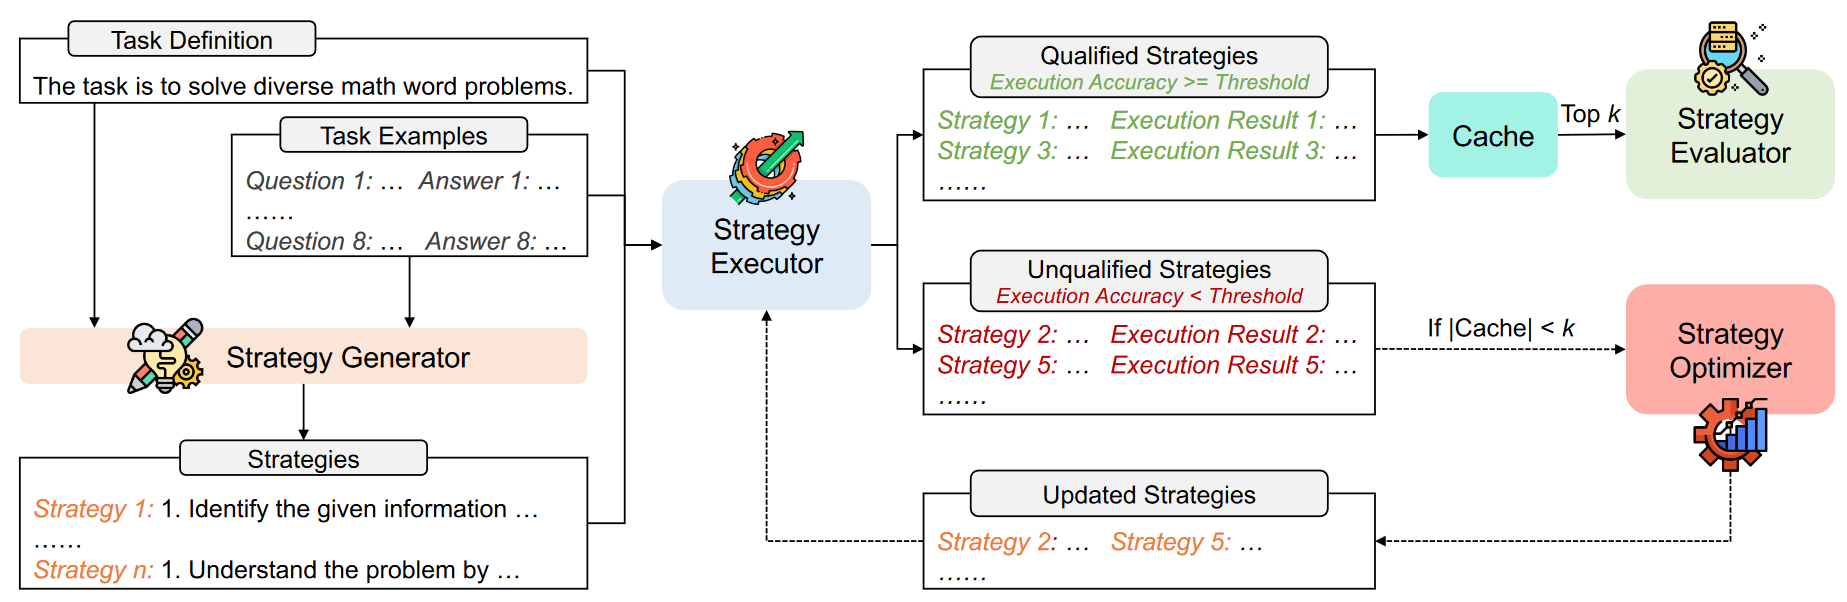
\includegraphics[width=0.9\linewidth]{StrategyLLM.png}
	\caption{StrategyLLM \cite{gao_strategyllm_2024}}
	\label{fig:strategyllm}
\end{figure}
This approach automatically constructs few-shot prompts and  needs no  human annotated examples. Bu it needs more tokens than CoT because generated prompts seem to be  often longer than human-written CoT prompts
\begin{figure}[h]
	\centering
	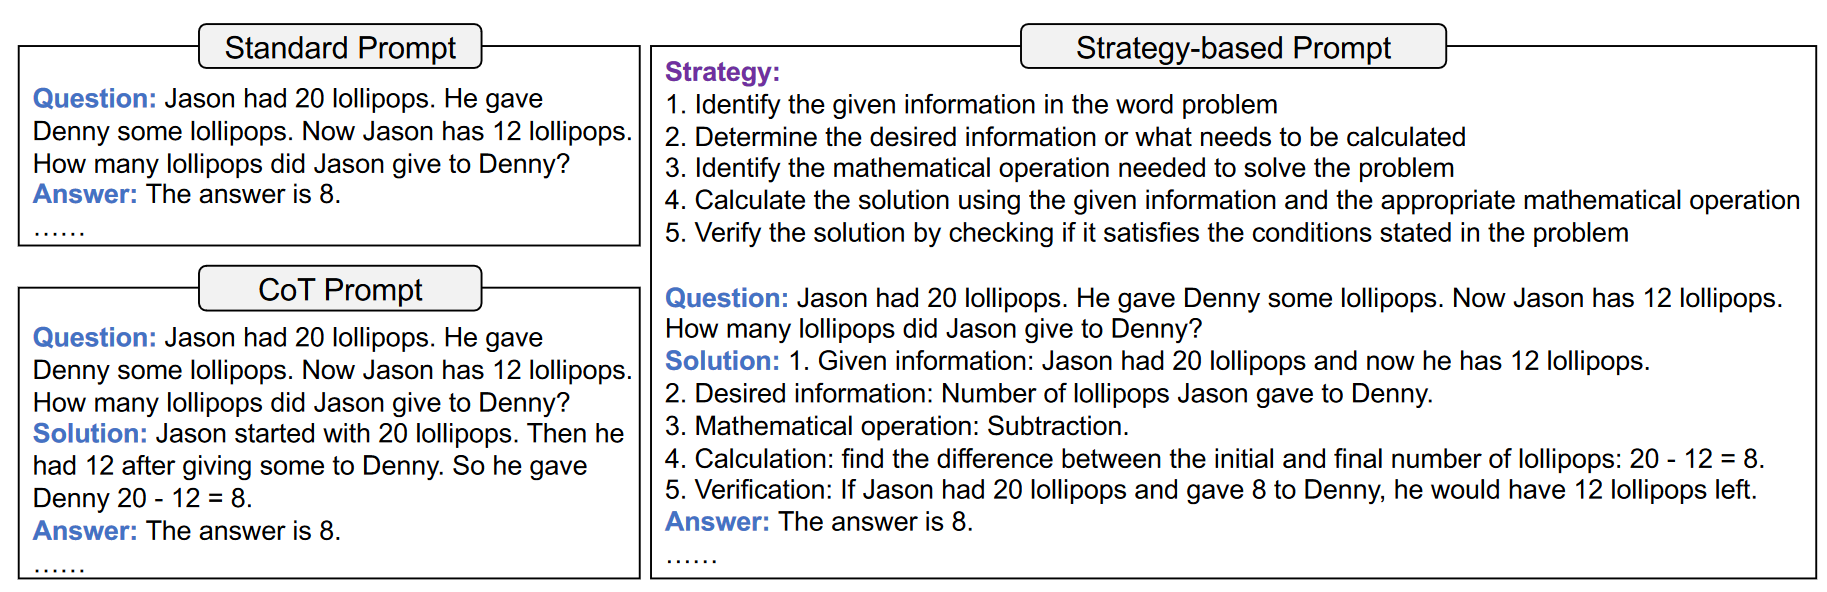
\includegraphics[width=0.9\linewidth]{StrategyLLM-StrategyBasedPrompt.png}
	\caption{StrategyLLM-StrategyBasedPrompt.png \cite{gao_strategyllm_2024}}
	\label{fig:strategyllmprompt}
\end{figure}
This approach demonstrated superior performance compared to CoT with self-consistency (which necessitates human annotation of solutions) in mathematical reasoning, common sense reasoning, algorithmic reasoning, and particularly in symbolic reasoning. The results were obtained using GPT-3.5-Turbo and GPT-4. GPT-4 yielded superior outcomes. It is notable that there is limited transferability of strategies between different LLMs.

%\cite{noauthor_agentgptgpt_nodate} is just AUtoGPT running in Web
%\cite{du_anytool_2024} AnyTool: Self-Reflective, Hierarchical Agents for Large-Scale API Calls

TODO: RELEVANT? 
\cite{raman_cape_2023} 22.10.2023 planning few-shot??
Planning LLM: demonstration set: high-level example task and respective plan, cosine similarity qith query task, generate actions for task
Translation LLM: Sentence-BERT LLM, embed free form actions (nat language) to semantically similar actions in agent's repertoire. step by step: append action, further autoregressive steps

TODO include example from robotic action plan, eg inner monologue \cite{huang_inner_2022}
Example of example plan:
\begin{verbatim}
	Task: Put objects in their corresponding bowls 
	
	Scene: Visible objects are ["red block", "green block", "red bowl", "green bowl"] 
	Scene: Occluded objects are [] 
	Robot action: robot.pick_place("red block", "red bowl") 
	Successful action: False 
	
	Scene: Visible objects are ["red block", "green block", "red bowl", "green bowl"] 
	Scene: Occluded objects are [] 
	Robot action: robot.pick_place("red block", "red bowl") 
	Successful action: True 
	
	Scene: Visible objects are ["red block", "green block", "red bowl", "green bowl"] 
	Scene: Occluded objects are [] 
	Robot action: robot.pick_place("green block", "green bowl") 
	Successful action: True 
	
	Scene: Visible objects are ["red block", "green block", "red bowl", "green bowl"] 
	Scene: Occluded objects are [] 
	Robot action: robot.stop() 
	STOP
\end{verbatim}

%"Zou et al. (2023) proposed AuRoRA, an augmented reasoning and refining system with task-adaptive CoT prompting"

\paragraph{Branching Task Sequences}
TODO: BRIEF INTRO

\subparagraph{Single Path}

TODO: INTRO 
Task: several steps, one path (eg linearly ordered)

TODO: REFER TO THE PROMPTING APPROACHES AND TO APPLICATIONS MENTIONED IN OPEN-LOOP PLANNING


short repetition/reference to CoT: 
\cite{kojima_large_2023} and all the improvements, self-ask \cite{press_measuring_2023} , contrastive CoT \cite{chia_contrastive_2023} ....

+ refer to the open-loop planning and some replanning approaches!

%CoT, for reasoning ability of LLM, generate intermediate reasoning steps
%include rationale for demonstration examples, series of intermediate reasoning steps, solve task in step-by-step manner

\subparagraph{Multi Path with Discriminator}
DRAFT: ONLY NOTES

TODO INTRO structure, generation + selection/ranking, 
choices, structures: multiple parallel paths/tree-like/graph, 
idea: several possible ways to solve problem, 
can explore more potential solution, select most promising or try several, 
but needs more computations/more resources, 
how to evaluate/rank tasks/which to choose? - needs discriminator

APPROACH1: PARALLEL PATHS; TRAINED PLAN RANKER

\cite{logeswaran_few-shot_2022} 27.05.2022 Few-shot Subgoal Planning with Language Models, multi-path!
LLMS can infer detailed subgoal sequences, only need few training examples and no finetuning
ALFRED benchmark
plan execution: pre-trained low-level policy available and state representation is provided (both assumed). feedback from environment: task success/failure. Use feedback to train a ranking model that re-ranks LLM prediction
subgoal inference: semantic parsing. text instruction to sequence of subgoals, predict sequence of subgoals
in-context learning
Lm predicts several subgoal sequences, re-rank to a ranked list of subgoal sequence, execute next subgoal from highest ranking plan
observations: update state representation
environment feedback: train supervised plan ranking model based on information from environment/environment feedback/execution of plans and success/failure outcomes of the plans in the environment: construct labelled dataset of instructions with corresponding plans and agent states, significant improvement

Multiple CoTs (CoT-SC): multiple parallel CoTs, select 1, here Self-consistency \ref{SC}
ref: many prompting approaches can be combined without changes with self-consistency!
 \cite{wang_self-consistency_2023} 07.03.2023 title: SELF-CONSISTENCY IMPROVES CHAIN OF THOUGHT REASONING IN LANGUAGE MODELS
increased temperature setting, diverse outputs/trajectories
increased performance in arithmetic and common-sense reasoning tasks
not greedy decoding. samples several reasoning paths from language model via CoT, trying to find most consistent answer: majority vote, significantly improved Cot?
"replace the naive greedy decoding used in chain-of-thought prompting"
sample diverse set of reasoning paths, select most consistent answer
"boosts the performance of chain-of-thought prompting with a striking margin on a range of popular arithmetic and commonsense reasoning benchmarks"
"intuition that complex reasoning tasks typically admit multiple reasoning paths"
"determine the optimal answer by marginalizing out the sampled reasoning paths to find the most consistent answer" idea: if multiple different ways of thinking lead to answer, more confidence that its correct
"The self-consistency method contains three steps: (1) prompt a language model using chain-of-thought (CoT) prompting; (2) replace the “greedy decode” in CoT prompting by sampling from the language model’s decoder to generate a diverse set of reasoning paths; and (3) marginalize out the reasoning paths and aggregate by choosing the most consistent answer in the final answer set"
\begin{figure}[h]
	\centering
	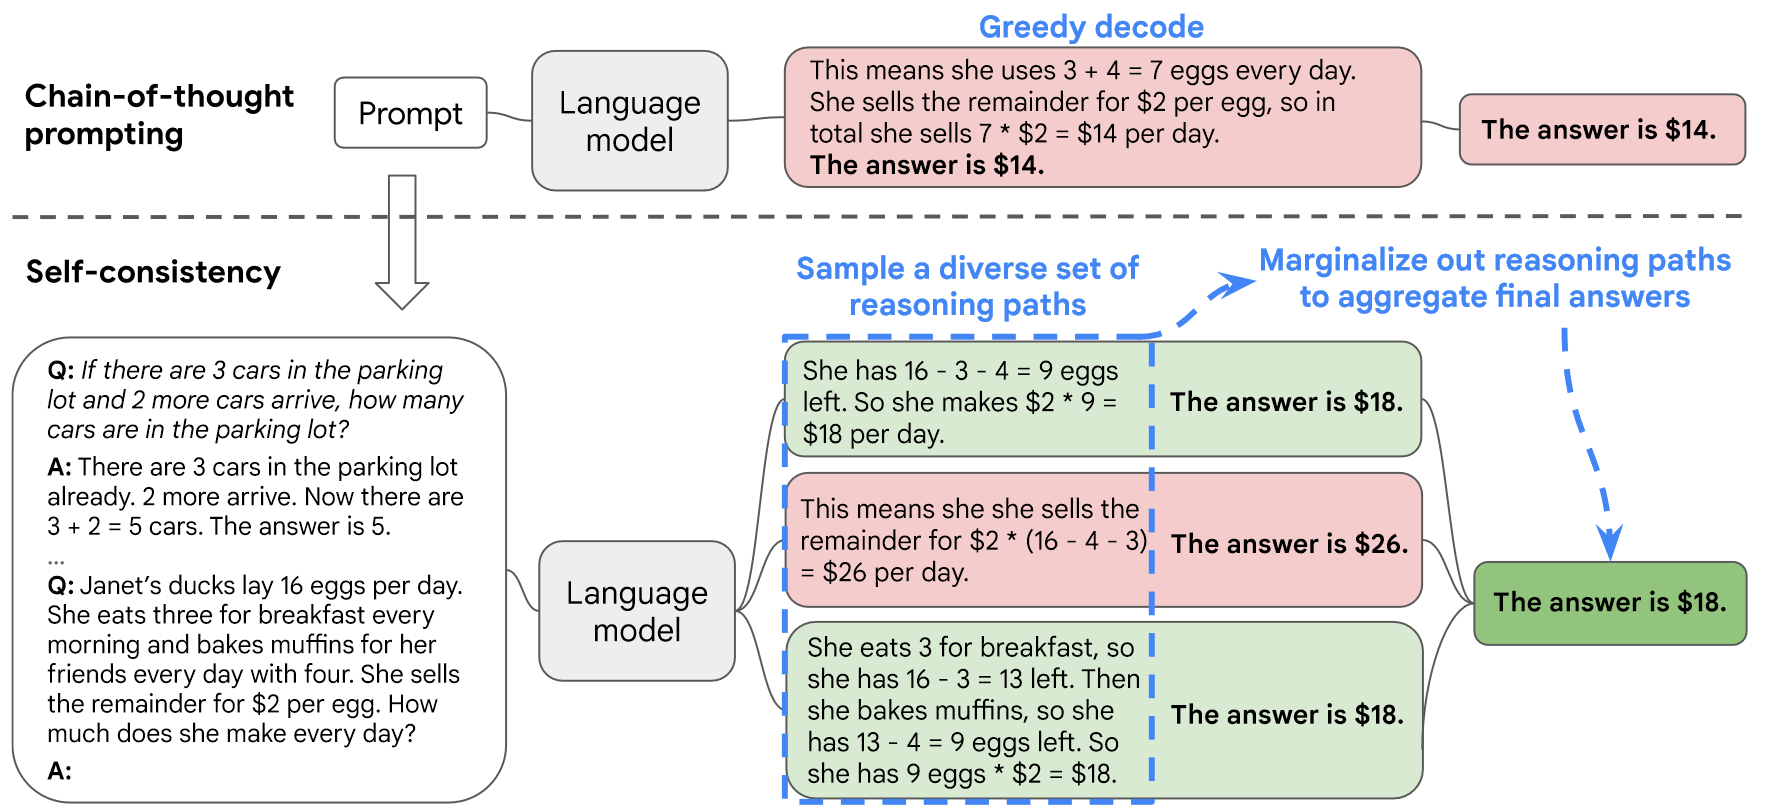
\includegraphics[width=0.7\linewidth]{SelfConsistency.png}
	\caption{SelfConsistency  \cite{wang_self-consistency_2023}}
	\label{fig:selfconsistency}
\end{figure}
directly applicable
"One should note that self-consistency can be applied only to problems where the final answer is from a fixed answer set, but in principle this approach can be extended to open-text generation problems if a good metric of consistency can be defined between multiple generations, e.g., whether two answers agree or contradict each other."
"find that self-consistency robustly improves reasoning accuracy for every language model"
UL2, GPT-3 code-davinci001 and code-davinci-002, LaMDA-137B, PaLM-540B
best GPT-3 code-davinci-002 and PaLM-540B
"incurs more computation cost", can check how many paths necessary

APPROACH2:TREE + TREE SEARCH

Tree of thought
\cite{long_large_2023}14.05.2023 Large Language Model Guided Tree-of-Thought
explores the solution space through a tree-like thought process, trial and error, backtracking
modules: prompter agent, checker module, memory module, ToT controller
multi-round conversation with the LLM
memory module: allows to save history and backtracking
tested: only on Sudoko Puzzle?
\begin{figure}[h]
	\centering
	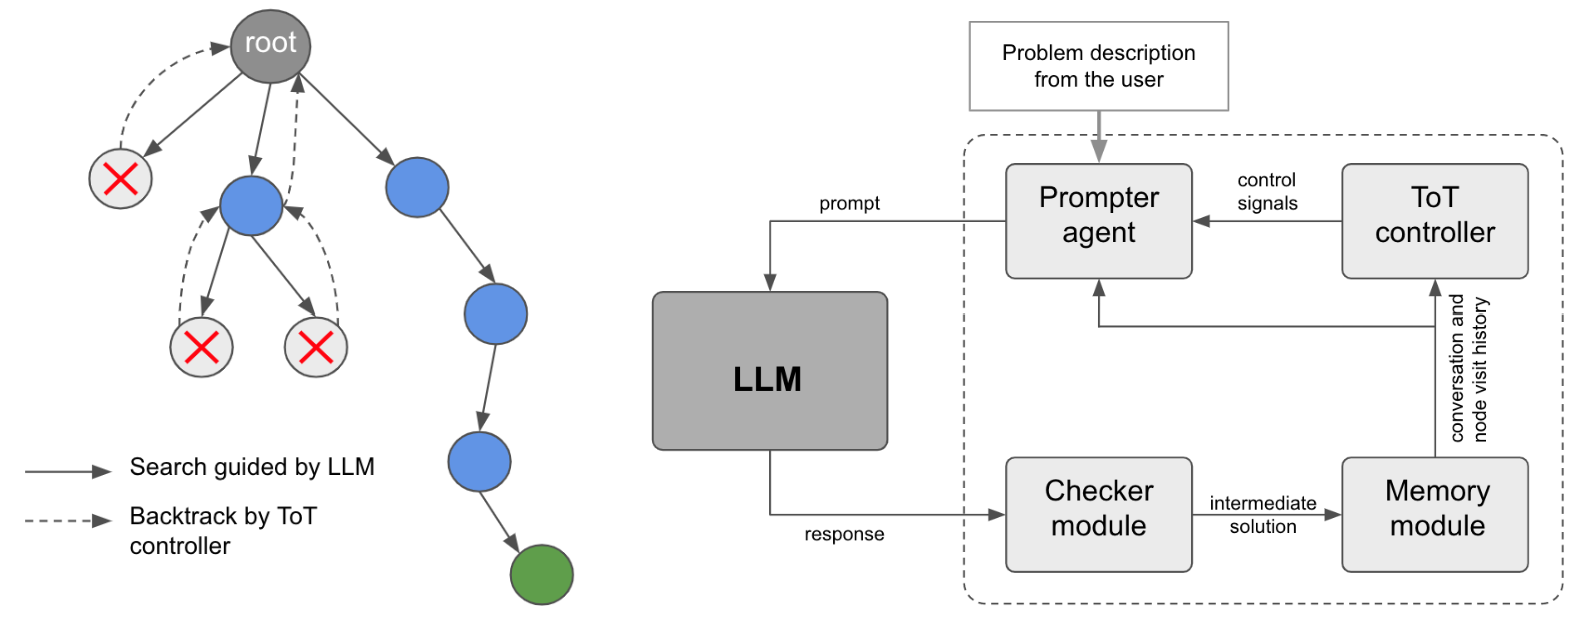
\includegraphics[width=0.7\linewidth]{TreeOfThought.png}
	\caption{TreeOfThought \cite{long_large_2023}}
	\label{fig:treeofthought}
\end{figure}
prompter: encourage LLM o produce intermediate solution, of correct stored in memory
prompter agent based on memory: next step
if invalid, prompt LLM to consider again
controller monitors whether to continue search from current node or backtrack
tree search, with LLM as heuristic
Checker module: problem dependent, check validity of intermediate solution -- assumption that it can be effectively checked!!
Memory module: history of conversation between LLM and prompter agent +  optional information
ToT controller: steers tree search, valid solution: explore children, otherwise backtrack, can alternatively use policy network to determine a backtracking policy
Prompter agent: templates for prompting LLM,
generic template:
\begin{verbatim}
	For the given problem: [problem description], we have come up with a partial solution: [partial solution summary]. Please derive the next step on top of this partial solution, and return the next step in the following JSON format {next_step: <next_step>}
\end{verbatim}
problem description and partial solution summary: from memory
gpt-3.5-turbo

STATES, ACTIONS, SEARCH, TREE; MCTS
\cite{hao_reasoning_2023} 23.10.2023 RAP Reasoning via Planning, Reasoning with Language Model is Planning with World Model
LLM lack internal world model to predict the world state, therefore hard to simulate long-term outcomes of actions
deliberate planning: explore alternative reasoning paths, anticipate future states and rewards, iteratively refining reasoning steps
LLM as: world model, reasoning agent, build a reasoning tree
planning algorithm: based on MCTS
LLaMA-33B
build reasoning tree
world model: future outcomes, 
backpropagate estimated future rewards
2/4/6-step problems of Blocksworld, significantly more better than CoT
state description eg variable values
prompt to LLm to generate the next state
compared to CoT: augment reasoning steps with predicted world states
rewards for applying actions to states (reasoning steps), different possibilities, eg likelihood of action (produced by LLM/probability), confidence of state (LLM),self-evaluation by LLM “Is this reasoning step correct?”, Task-specific heuristics
based on world model, can use planning algorithms, here MCTS
demonstrations for action likelihood:
\begin{verbatim}
	I am playing with a set of blocks where I need to arrange the blocks into stacks. Here are the actions I can do 
	
	Pick up a block 
	...
	
	I have the following restrictions on my actions: 
	I can only pick up or unstack one block at a time. ...
	
	[STATEMENT] As initial conditions I have that, the red block is clear, the yellow block is clear, the hand is empty, ...
	
	My plan is as follows: 
	
	[PLAN] 
	unstack the yellow block from on top of the orange block put down the yellow block pick up the orange block
	[PLAN END]
\end{verbatim}
next state prediction: 
\begin{verbatim}
	<actions>
	<restrictions>
	After being given an initial state and an action, give the new state after performing the action. 
	[SCENARIO 1] 
	[STATE 0] I have that, the white block is clear, the cyan block is clear,... 
	[ACTION] Pick up the brown block. 
	[CHANGE] The hand was empty and is now holding the brown block, ... 
	[STATE 1] I have that, the white block is clear, the cyan block is clear, ...
	[SCENARIO 2]
	...
	[SCENARIO 3] 
	[STATE 0] <state> 
	[ACTION] <action> 
	[CHANGE]
\end{verbatim}

Tree of Thoughts (ToT): generate from given position and possibly backtrack, scored thoughts \cite{yao_tree_2023} 03.12.2023 Tree of Thoughts: Deliberate Problem Solving with Large Language Models
tree structure
node: thought-action pair
search with BFS or DFS
improvements in specific tasks (Game of 24, crosswords, creative writing)
can explore multiple possibilities of reasoning at eaxch step
"ToT allows LMs to perform deliberate decision making by considering multiple different reasoning paths and self-evaluating choices to decide the next course of action, as well as looking ahead or backtracking when necessary to make global choices"
enhances problem solving on Game of 24, Creative Writing, and Mini Crosswords
significantly outperformed CoT
\begin{figure}[h]
	\centering
	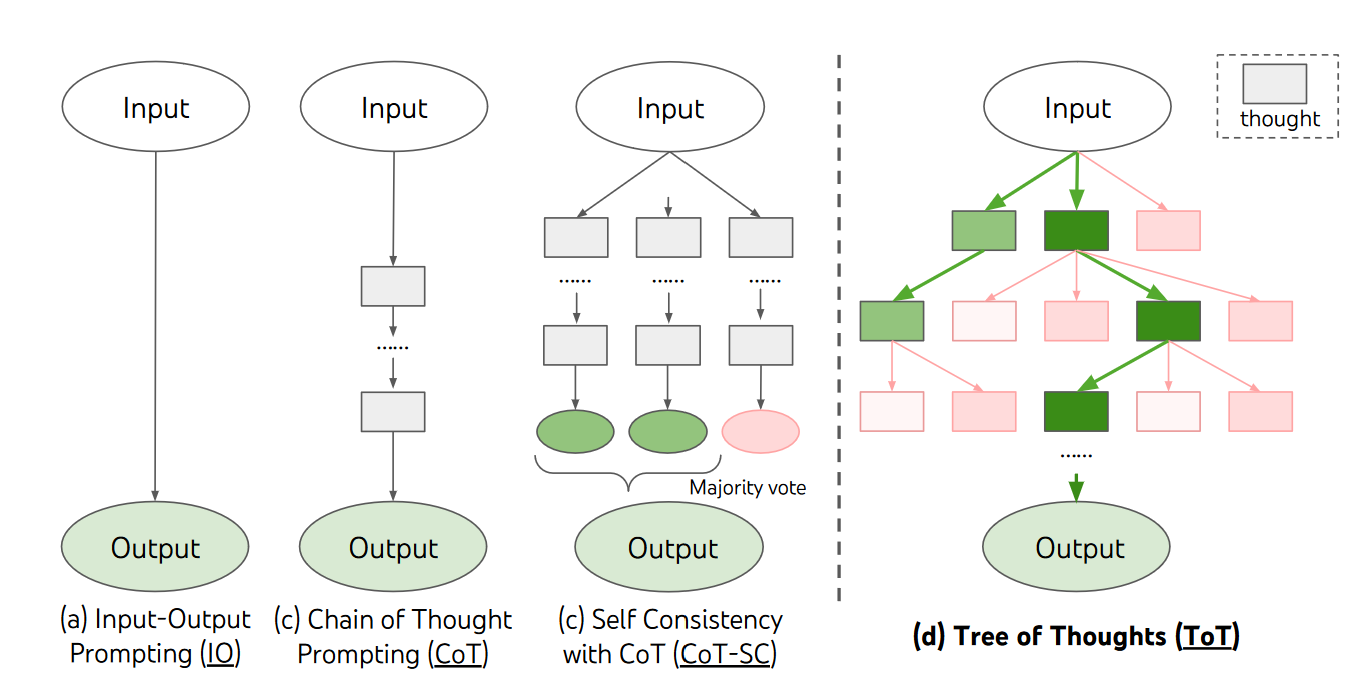
\includegraphics[width=0.7\linewidth]{ToTComparison.png}
	\caption{ToTComparison \cite{yao_tree_2023}}
	\label{fig:totcomparison}
\end{figure}
thought: coherent language sequence as intermediate step , explore different intermediate thoughts
implementation of search heuristics via LM self-evaluation and deliberation
LLM. generate and evaluate thoughts, BFS/DFS tree exploration with lookahead and backtracking
multiple reasoning paths, problem = search over tree, node = state, representing partial solution
generate next thought for next step:
Sample thought eg from CoT prompt or propose thoughts sequentially (propose prompt)
state evaluator: evaluate progress towards solving the problem (heuristic for search algorithm), two strategies: Value of each state independently (value prompt about scalar value of state, needs ability of LLM to be able to lookahead in this situation or reason via commonsense logic/knowledge inherent), or: vote across states/compare different states and vote for most promising one
outperforms CoT and CoT-SC by a very large margin
examples of evaluation prompts
\begin{verbatim}
	vote_prompt = '''Given an instruction and several choices, decide which choice is most promising. Analyze each choice in detail, then conclude in the last line "The best choice is {s}", where s the integer id of the choice.
	'''
	score_prompt = '''Analyze the following passage, then at the last line conclude "Thus the coherency score is {s}", where s is an integer from 1 to 10.
	'''
\end{verbatim}



STATES, ACTIONS, SEARCH
\cite{zhou_language_2023} 05.12.2023 LANGUAGE AGENT TREE SEARCH UNIFIES REASONING ACTING AND PLANNING IN LANGUAGE MODELS
LATS (Language Agent Tree Search), a general framework
inspired by monte carlo tree search
LLM: agent, value function, optimizer
external feedback from environment crucial?
self-reflection
external memory
expand ReAct, outperforms ReAct
introduce an LM-based Monte Carlo tree search variant to deliberately construct the best trajectory from sampled actions, using heuristics from LM
external feedback and self-reflection: learn from experiences
mitigate: autoregressive sampling like in CoT neglecting alternatives
Usually MCTS requires environment model
ReAct basis: receive observation , take action a following policy base on instruction+ggf few-shot examples
ReAct actions: permissible actions and reasoning traces (thoughts)
policy: $\pi(a_{t} | x, o_{1} \ldots o_{i-1}, a_{1} \ldots a_{i-1})$
sample n actions, assumption: for complex decision making tasks probably several correct trajectories/reasoning paths + mitigate stochastic text generation + greater exploration
MCTS: tree with nodes = states, of input and action and observations sequence
state: $s = [x, a_{1} \ldots a_{i}, o_{1} \ldots o_{i}]$
model-free
operations: selection, expansion, evaluation, simulation, backpropagation, and reflection,
selection: UCT algorithm
expansion: sample n actions, give to environment and get feedback as observation, add child nodes
evaluation: LLM reason about state, attribute scalar value for correctness of trajectory
simulate: until terminal state is reached, backpropagate value, self-reflection, eg unsuccessful terminal node about errors in reasoning or acting
Observe performance gain of using MCTS over variants like DFS
higher computational cost
for tasks where performance is more important than efficiency (eg programming?)
OWN ANALYSIS: valuable if actions take short time and are fully reversible! because several actions are actually executed! , sometimes no roll-back or high costs!

APPROACH3: GRAPH STRUCTURE

\cite{besta_graph_2023} 24.11.2023 Graph of Thoughts: Solving Elaborate Problems with Large Language Models
model LLM output information as graph:
information/thoughts=vertices, edges: dependencies between vertices
networks of thoughts, feedback loops
assumption: closer to human thinking
could merge chains of reasoning
model reasoning process as graph, networked reasoning
generalizes CoT and ToT, and also no model updates
modular architecture to implement GoT:
fine-grained control over individual thoughts and extendable (eg with other prompting ideas?)
where tasks can be decomposed into subtasks and solutions merged, GoT seems to outperform CoT and ToT by a large margin and reduce costs compared to ToT
\begin{figure}[h]
	\centering
	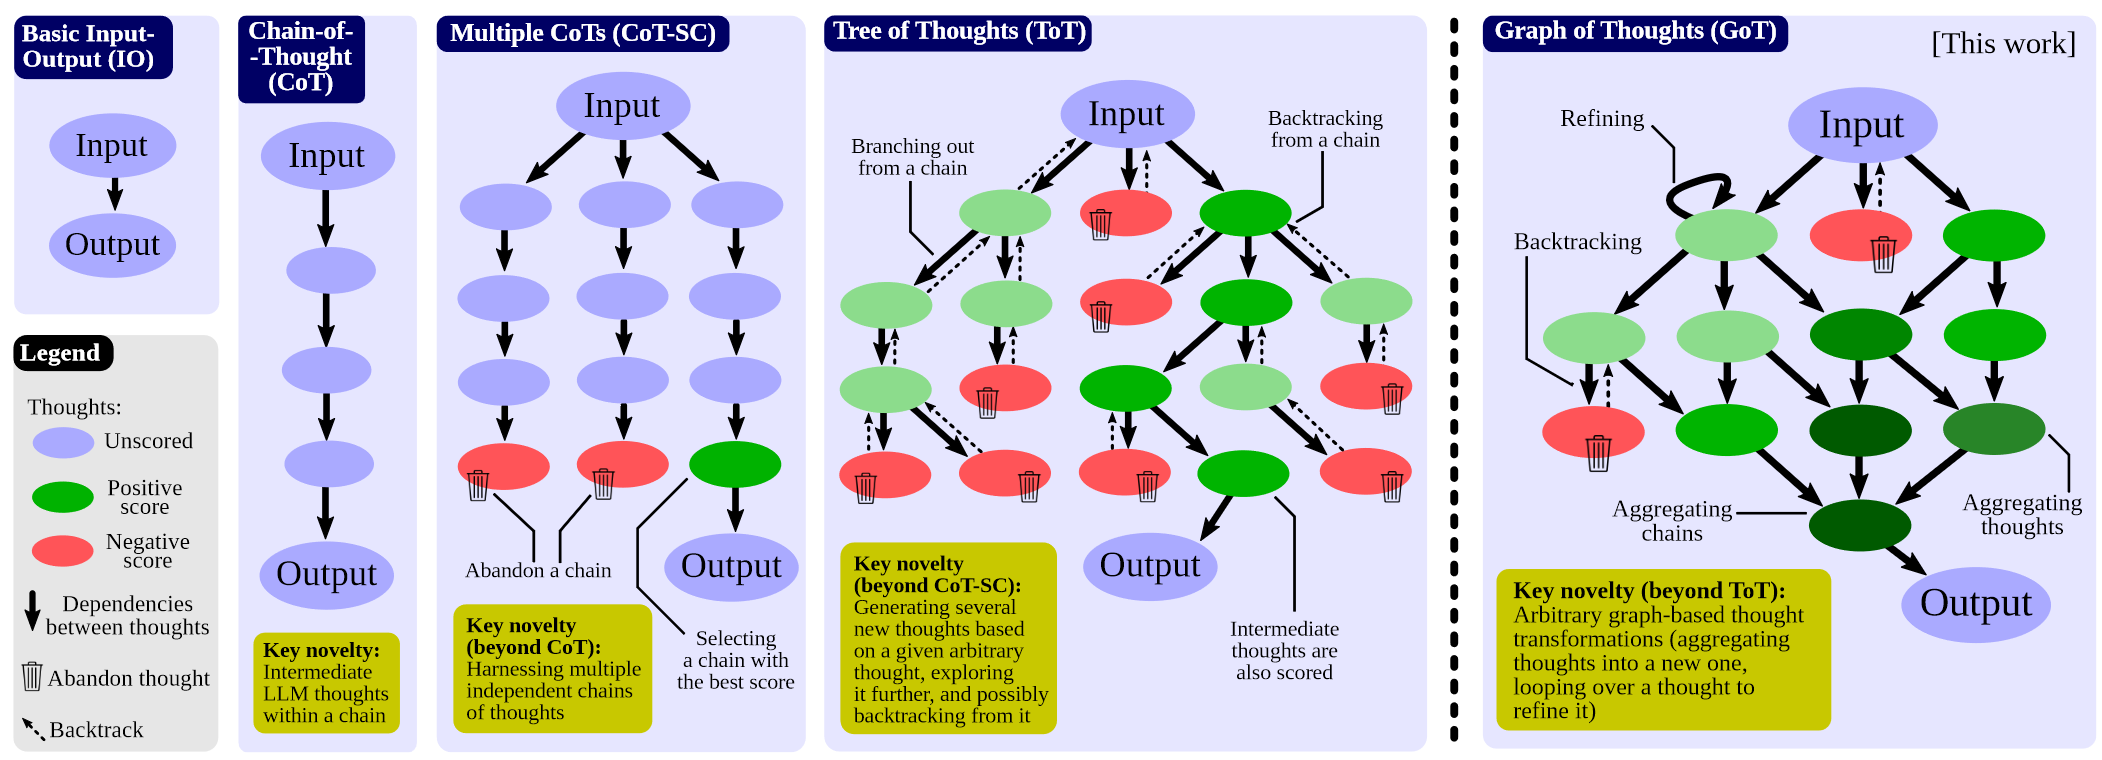
\includegraphics[width=0.7\linewidth]{GoT-Comparison.png}
	\caption{\cite{besta_graph_2023}  GoT compared to other single and multiple path prmpting strategies}
	\label{fig:got-comparison}
\end{figure}
can aggregate and generate thought aggregate: several thoughts leading to one/incoming to ne, generate: vertex from which several thoughts emerge
vertex: (partial) solution, different vertices can model different aspects of the reasoning process
can also loop over a thought and enhance it, can merge best thoughts, can aggregate whole paths of reasoning
thoughts are scored with a function, can also use function to rank thoughts
Architecture: prompter (prepares message), parser (extracts information from LLM reply), scoring module, controller (of reasoning process, decides about progression), controller contains: graph of operations(graph decomposition of task) and graph of reasoning state /history of reasoning process)
\begin{figure}[h]
	\centering
	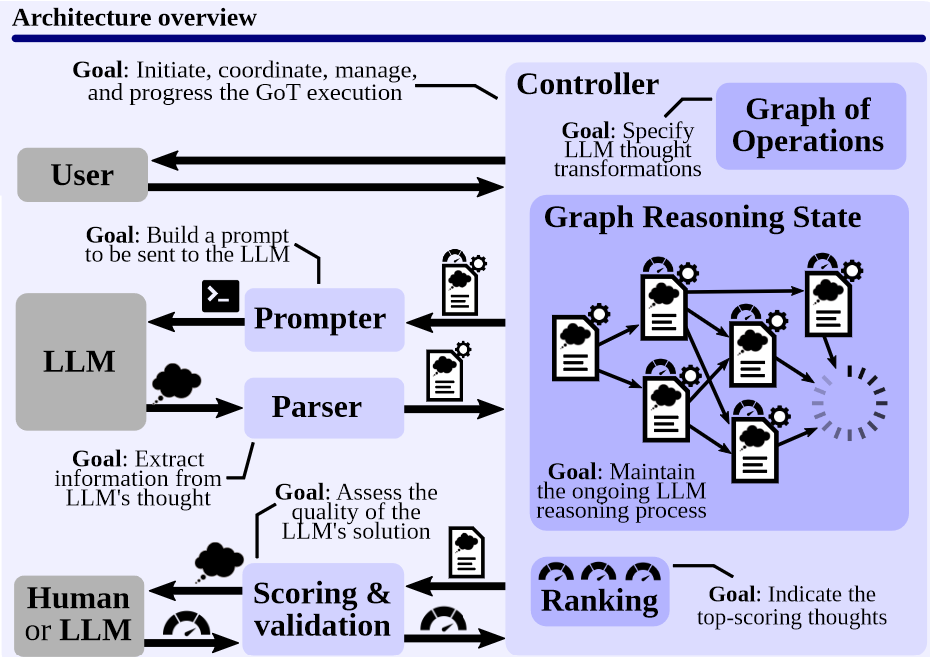
\includegraphics[width=0.7\linewidth]{GoT-Architecture.png}
	\caption{\cite{besta_graph_2023}  GoT general architecture overview}
	\label{fig:got-comparison}
\end{figure}
examples: good for tasks that can be split and the results merged, like sorting, set operations , keyword counting, document merging
GPT-3.5 (also tried Llama-2, but was always worse)
additional info:
graph-based structure (also: aggregations, self-loops)
TODO graphic of the paper comparing different multi-path methods and mentioning the key novelties
self-refine, eliminate nodes
can follow several paths
reduction in error rates for some tasks (sorting, set operations)
cut costs?!



%%%%%%%%%%%%%%%%%%%%%%%%%%%%%%%%%%

STATES, ACTIONS, SEARCH: encoded in decomposition
\cite{sel_algorithm_2023} Algorithm of Thoughts: Enhancing Exploration of Ideas in Large Language Models
multi path methods like ToT outperformed single path methods but need more queries
on goal: avoid too many model queries: monetary, latency, energy consumption --reduce the query counts employed by contemporary multi-query reasoning methods
instead of of [PROBLEM, SOLUTION] or [PROBLEM, SUCCESSIVE STEPS TO SOLUTION], present a new structure that covers [PROBLEM, SEARCH PROCESS, SOLUTION]
in-context examples patterned after search algorithms, notably depth-first search (DFS) and breadth-first search (BFS), tasks reminiscent of tree search problems
key components of tree search algorithms:
decomposition of a problem into sub problems including interrelations between subtasks and the complexity of subtasks
solution proposal to subproblems
gauging promise of a subproblem/potential/promising routes
backtracking
AoT surpasses other single prompt methods like  CoT/-SC prompting and competitive to ToT, but significantly less queries than ToT, but longer input than CoT
Disadvantage: authors gave comprehensive demonstration (1 demonstration, but like tree search, decomposing into subproblems and backtracking) of exactly the task the model was supposed to solve and examples how to solve the task by search similar procedure

GENERAL: DISCRIMINATOR
\cite{chen_when_2024} When is Tree Search Useful for LLM Planning? It Depends on the Discriminator
multi-step LLM planning
iterative generation/generator: at each step, search for possible next action, generate language representations
discrimination/discriminator: predict outcomes of actions (rewards, correctness)
planning: incorporate outcome into problem-solving process, strategy to find best action sequence
planning methods tested: re-ranking, interative correction, tree-search
"te discriminators with different levels of accuracy. The simulation experiments exhibit a strong correlation between discrimination accuracy and overall task performance among all three types of planning methods. Then, in a non-oracle setting, we closely investigate the LLM-based discriminators and show how environmental observations can effectively improve them"
"Advanced planning methods, i.e., iterative correction and tree search, demand highly accurate discriminators ($\geq 90\%$ accuracy) to achieve decent improvements over the simpler method, re-ranking."
"compared to the other two methods, tree search is at least 10–20 times slower but leads to negligible performance gains"
compare:
-generate and rerank (generator generates complete action sequences, discriminator scores them)
-iterative correction (generator provides complete plan/action sequence to discriminator, discriminator provides feedback, several rounds of correction possible, here: also scoring and revision o best plan, zero-shot instruction for plan revision)
-tree search (generator proposes new steps for current best partial plan, discriminator evaluates steps and updates tree, here MCTS like implementation)
generator:  CodeLlama-13BInstruct
discriminators: CodeLlama-7B-Instruct and CodeLlama-13B-Instruct, closed: GPT-3.5-Turbo (OpenAI, 2022) and GPT-4-Turbo (OpenAI, 2023), and (3) fine-tuned LLMs: CodeLlama-7B-Instruct-FT and CodeLlama-13B-Instruct-FT
Observation from experiments:
"Advanced planning methods demand highly accurate discriminators."
"Advanced planning methods may not adequately balance accuracy and efficiency. By calculating the average inference time per example (Figure 3), we find that our implementation of tree search is at least 10–20 times slower than the other two planning methods"
"Monte-Carlo tree search can be unstable, especially in the early stages"
LLMs as discriminators: "closed source LLMs exhibit stronger discrimination abilities, with GPT-4 achieving the best performance", next finetunded CodeLlama-13B-FT and GPT-3.5-Turbo, but CodeLlama-13B/7B at least not that far behind
propose to add program executability checks into feedback (score 0 if not executable), notable improvement with such environment feedback
observe more than 50\% discrimination errors (eg high ranking of not best choice etc)
"For these reasons, iterative correction and tree search cannot gain decent improvement over reranking with the same LLM-based discriminator."
Me: seems that decisive criterion in these tree based approach is a good discriminator 8heuristics/ranking), not the tree search method itself!!


\subsubsection{Planning via Symbolic Planner}
DRAFT: ONLY NOTES

INTRO NOTES: 
avoid the usual huge drawback of symbolic approach in model building, 
theoretical advantages: completes, interpretability, stability?,...
But: translation..errors... then with only small error no planning, translation of vague text into symbolic model, potentially ambiguity, 
when having constraints, all respected but also all have to be declared explicitly

mention? Elaboration Tolerance McCarthy98 ->small change in problem -> small change in representation???

How to combine LLM+symbolic approache? -  is taken as translation task: translate natural language into PDDL, call solver, 
What to translate into PDDL: Goal (need domain + problem file), problem file, all

SIMPLEST APPROACH: ONLY TRANSLATE GOAL TO PDDL
\cite{xie_translating_2023} 10.02.2023 Translating Natural Language to Planning Goals with Large-Language Models
"recent work has also shown that LLMs are unable to perform accurate reasoning nor solve planning problems,"
more effective at translation than at planning
"central question is whether LLMs are able to translate goals specified in natural language to a structured planning language"
LLM as interface between planner and human user
GPT-3.5 for our experiments, specifically code-davinci-002 for all Blocksworld tasks and text-davinci-003 for ALFRED-L
"variants show that LLMs are much better suited towards translation rather than planning"
under-specified goals in natural language
ability to generate goals depends on domain (hard in numerical or physical reasoning) and sensitive to prompts
extract a planning goal from given a natural language instruction
udr effective classical planners
translation from natural language to PDDL, needs: contextual information, prior knowledge
+ needs correct syntax of PDDL, and compatibility with domain and problem information
Blocksworld, ALFRED
prompt must consist of: Domain PDDL, One-Shot Problem PDDL, One-shot Language Instruction, One-shot Goal PDDL, Test Problem PDDL,Test Language Instruction
ONLY GENERATES THE GOAL!!!
very sensitive to prompt, eg if Blocksworld positions are described from top to bottom instead of bottom to top 
partial goal specification: LLM able to apply commonsense reasoning to fill gaps (with daily/common objects and relations)
tests to test understanding of the domain showed that probably LLM not able to understand physical world semantics of predicates
works mainly through goodl and many example prompts and therefore linguistic capabilities

CREATE MOST OF PDDL PROBLEM FILE/ TRANSLATE GOAL AND STATES
\cite{dagan_dynamic_2023} 11.08.2023 planning via neuro-symbolic+ online replanning
context window vs complex plans with multi-step reasoning
planning: effects of actions, states, goal state
symbolic planners: optimal solution BUT need planning problem complete and accurate description
LLMs: noisy observations, uncertainty
LLM Dynamic Planner (LLM-DP): a neurosymbolic framework, LLM+traditional planner
ALFWorld
LLMs: hallucinations (incorrect or spurious information) + dependent on prompt formulation
LLM iterated invocations: high computational costs
symbolic planners: if domain and problem description existent, efficient in optimal plan search
but descriptions hard to get, sometimes not existent
LLM. understands actions and impact on environment, planner finds solution
LLM-DP: high level process
LLM observations + natural language instructions parse into PDDL, generates predicates for objects (semantic and pragmatic inference), sample possible predicates: multiple plans possible. Action selector decides about action or review problem or as questions
\begin{figure}[h]
	\centering
	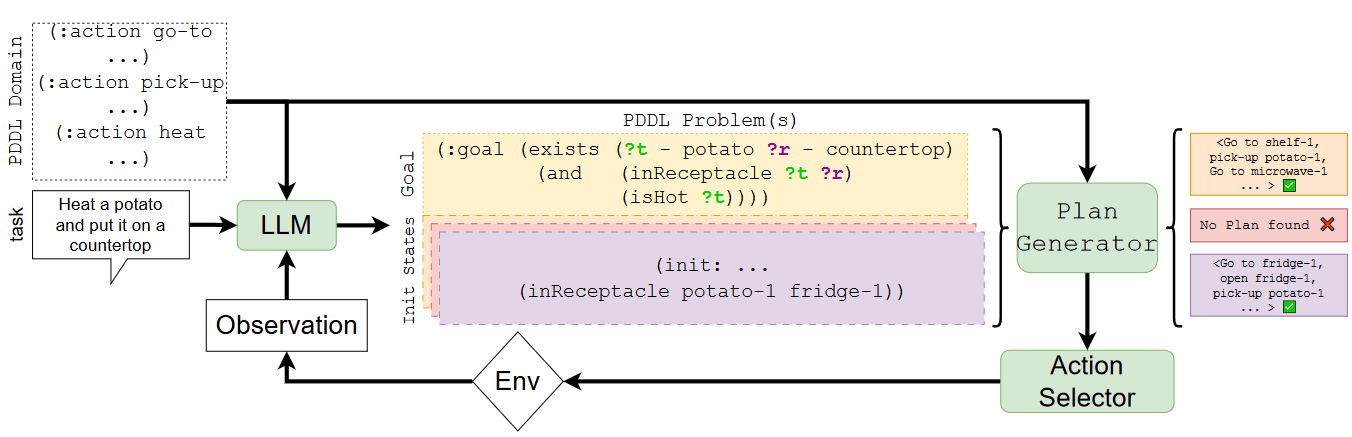
\includegraphics[width=0.9\linewidth]{LLM-DP}
	\caption{LLM-DP \cite{dagan_dynamic_2023} }
	\label{fig:llm-dp}
\end{figure}
tracking of world state W and beliefs B about predicates in environment
W World all known information
beliefs: set of possible valid predicates, can be true or false
With W and B construct different planning problem PDDL files with: objects observed, current state and goal
LLM samples from B, Known world state + options for predicate to LLM, LLM completes the state
random sampling vs LLM sampling: same average accuracy!
use traditional solver (here BFS(f))(Lipovetzky et al., 2014, plan = sequence of actions (symbolic) (=classical planning)
LLM: translates task description into goal state, sample beliefs to generate plausible world states
Assumptions: 
-Need PDDL domain file: available actions with pre- and post-conditions and existing predicates
-perfect observations
-causal environment (static, inertial?, only changed by agent)
-valid actions always succeed
gpt-3.5-turbo-0613 LLM model with a temperature of 0
compared to ReAct significantly higher average accuracy and most significantly/extremely less LLM tokens used (LLM-Dp 633k vs on ReAct implementation 9.16M)
Action selector: planner's output is set of plans. Select action from the plans. here: select actions from shortest plan
if no valid plans found: could use self-reflection to update beliefs, or human-agent interaction
Observations: symbolic action effects lead to change of state representation +  observation to update state and beliefs, new information: trigger re-planning process
One of the few-shot examples for generating the goal
\begin{verbatim}
	Your task is to: put a clean plate in microwave. 
	(:goal (exists (?t - plate ?r - microwave) 
	(and (inReceptacle ?t ?r) 
	(isClean ?t) )))
\end{verbatim}
excerpt from predicate definition for generating the goal
\begin{verbatim}
	(define (domain alfred) 
	(:predicates 
	(isReceptacle ?o - object) ; true if the object is a receptacle 
	(atReceptacleLocation ?r - object) ; true if the robot is at the receptacle location
	...
\end{verbatim}

TRANSLATE WHOLE PROBLEM FILE TO PDDL
transform planning problem to PDDL planning problem file
\cite{liu_llmp_2023} 27.09.2023 LLM+P: Empowering Large Language Models with Optimal Planning Proficiency
long-horizon robot planning problems
vs classical planners: efficient search algorithms
issue: need formal problem description
input: natural language description of planning problem, returns correct or optimal plan in natural language
convert into PDDL, use classical planner, translate back
LLM+P in robotic domains can often find optimal solution vs pure LLM which most times fail to produce feasible plans
Why not use specialised tools like symbolic planners , they are available, connect LLM to planner as tool
not altering LLM
classical planning problem, plan = sequence of actions, PDDL, standardized encoding of classical planning problems
assumption: domain rules are available, needed: already existing PDDL planning domain file! "we assume that for each problem domain, a human expert can provide a domain description (i.e. action preconditions and effects)"
assumption: LLM may be bad at planning but good at translating natural language input to PDDL formal format, like a machine translation task
GPT-4, even without prompt engineering almost useable
use in-context learning, demonstrations, give an example of natural language problem description and its PDDL representation, then GPT-4 able to directly translate to PDDL (in article they use only simple blocksworld and very comprehensively formulated problem description!)
LLM alone: lacks reasoning about preconditions, cannot keep track of properties, large number of LLM calls in long-horizon problems
LLM+P can produce optimal plan (due to solver!), but needs demonstration to produce valid PDDL file
\begin{figure}[h]
	\centering
	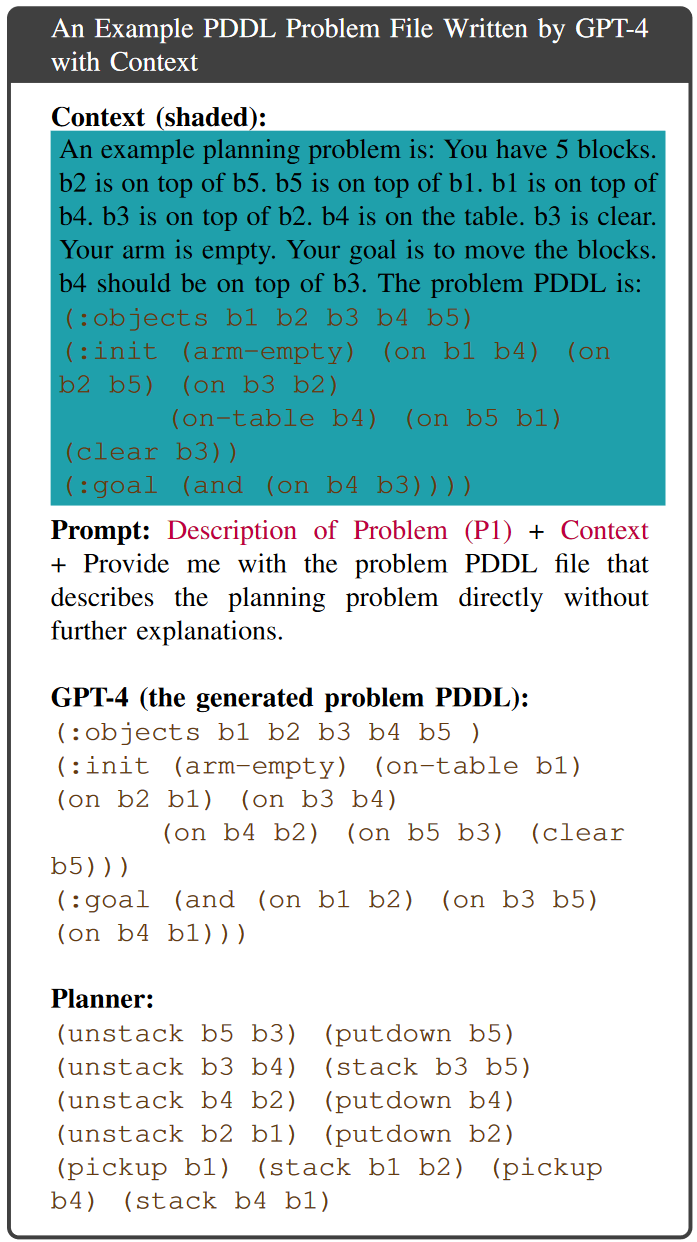
\includegraphics[width=0.4\linewidth]{LLMplusPGeneratedProblem.png}
	\caption{LLM+P Generated Problem \cite{liu_llmp_2023}}
	\label{fig:llmpluspgeneratedproblem}
\end{figure}

GENERATE PDDL DOMAIN AND PROBLEM FILE
!!! NOT ONLY translate goal to PPDL requiring handcrafted PDDL domain model, but also generate domain model:
\cite{guan_leveraging_2023}
problems with pure LLM planning: limited correctness of plans, strong reliance on environment feedback, inefficiency in using human feedback
here: construct explicit world/domain model in PDDL, can then use domain-independent planners
"involves maintaining an explicit world model instead of directly mapping user prompts to plans"
LLMs as interface between PDDL + sources of feedback (PDDL validators, humans)
human involvement: at beginning in supporting domain model generation, not needed later for feedback on planning
GPT-4
LLM may overlook physical plausibility of actions, not effective in long-term dependencies
LLMs still not reliable planners (to produce correct and executable plans)
improvement by feedback: need simulator or fully online, during executing the plan
model-based paradigm instead
actions + brief natural language description, LLMS: extract symbolic representation to PDDL action model
human feedback: translate PDDL in natural language, get natural language feedback, translate back to PDDL
GPT-4 was able to generate high-level domain models
translate user instruction to PDDL goal specification
can also use in other way: PDDL model to validate plan generated by LLM, provide corrective feedback (preconditions), PDDL model= "simulator"
skill library, skill and short description, low-level control policies of skills available
generate sequence of high-level skills
PDDL: standard encoding language for classical planning problems
\begin{figure}[h]
	\centering
	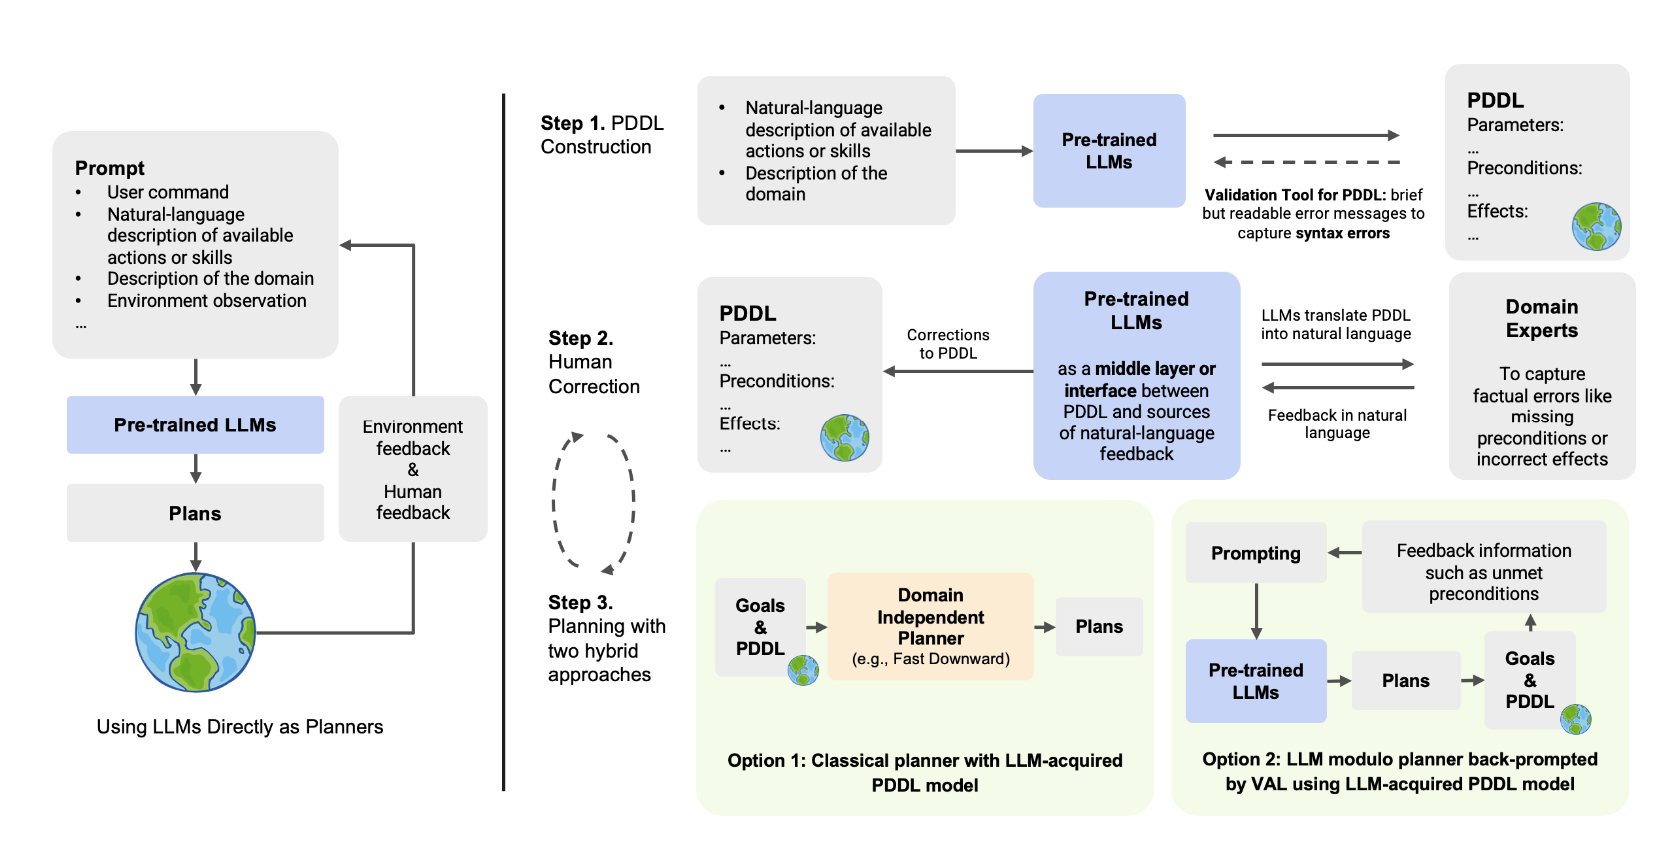
\includegraphics[width=1.0\linewidth]{PDDLTranslationFramework.png}
	\caption{PDDLTranslationFramework 
		\cite{guan_leveraging_2023}}
	\label{fig:pddltranslationframework}
\end{figure}
Prompt to translate the domain:
\begin{verbatim}
	<Instructions for the PDDL generation task>
	You are defining the preconditions and effects (represented in PDDL format) of an AI agent's actions. Information about the AI agent will be provided in the domain description ... 
	<One or two examples from other domains for illustrating the input and output formats>
	Here are two examples from the classical BlocksWorld domain for demonstrating the output format. ... Here is the task. 
	<A natural language description of the domain> 
	Domain information: The AI agent here is a household robot that can navigate to various large and normally immovable furniture pieces or appliances in the house to carry out household tasks ... 
	<A natural language description of the action> 
	Action: This action enables the robot to toggle small appliances (like humidifiers and light bulbs) which are toggleable to switch them on ...  
	<The dynamically updated list of predicates> 
	You can create and define new predicates, but you may also reuse the following predicates: 1. (robot-at ?r - robot ?f - furnitureAppliance): true if the robot ?r is at the furniture or appliance ?f  ... 
	Parameters:
\end{verbatim}
iterate over generation to identify preconditions
feedback sources: PDDL model validation tools (e.g., the one in VAL [18], human domain experts
Generating plans using PDDL  model: 2 options:
1) Classical planner with LLM-acquired PDDL model, eg Fast Downward
2) LLM modulo planner backprompted by VAL using LLM-acquired PDDL model; iteratively refine LLM plan through feedback from "simulator" and re-prompting
"GPT-4 can produce high-quality PDDL models with significantly fewer errors when compared to GPT-3.5-Turbo"
LLMs lack reasoning skills of causal relationships when constructing PDDL
also feedback/correction dependent on GPT-4, 3-5 not that useful
Comparison of success rates in household and logistics domain: Only LLM planner barely able to find executable plans,  LLM backprompted by VAL using LLM-acquired PDDL model significantly better, but approach of Fast Downward with LLM-acquired PDDL model finds feasible plan in 95\%-100\% successful
advantages of this approach: safety concerns of LLM plans? Human can correct domain model, improved explainability
construct PDDL action by action because of restricted context window size



%\cite{izquierdo-badiola_plancollabnl_2024} PlanCollabNL: Leveraging Large Language Models for Adaptive Plan Generation in Human-Robot Collaboration
%"LLMs as translators between NL information and a structured AI task planning problem, targeting humanrobot collaborative plans"
%Human-Robot Collaboration (HRC) ,generate an executable HRC plan with specific subgoals and an appropriate task allocation

TODO: 
Check: Romero e. a. Synergistic Integration of Large Language Models and Cognitive Architectures for Robust AI: An Exploratory Analysis 2308.09830v3


\subsubsection{Planning via Neural Planner} \label{PlanningModuleNN}
DRAFT: ONLY NOTES

\cite{gur_real-world_2023} WebAgent: introduce own model HTML-T5 "HTML-T5, a domain-expert pre-trained language model, for task planning and conditional HTML summarization" captures syntax and semantics of HTML pages, "introduce self-experience supervision, where the domain-expert language models are finetuned with self-generated demonstrations"
specialized model for HTML, finetuned with environmental feedback to remove critical failures
finetuning for planning and summarization
web automation good example for planning interaction with pages for task fulfilment often requires long-horizon planning, depending on use case, they: real-estate search 20 steps per episode
describe that with supervised experience, programming and summarization errors decreased, but planning especially long-horizon remains difficult
domain-expert language model + self-experience data
finetuned for planning, predicts next subinstruction given instruction history and current HTML data
Eval: surely perfect for the use case web automation, where page structure must be understood dynamically

TODO: ADD?
SwiftSage \cite{lin_swiftsage_2023}, adds offline imitation learning, BUT: needs oracle paths!!
general idea of a Decision Transformer Chen et al., 2021 https://arxiv.org/abs/2106.01345
Combine language model for action generation and RL model for choosing/evaluation: CALM Yao et al., 2020 https://arxiv.org/abs/2010.02903

\subsubsection{Planning Approaches}
DRAFT: ONLY NOTES

\paragraph{Classical Open-Loop Planning}

TODO INTRO: 
offline (complete, immutable plan) 
also called open-loop systems 
pre-determined plans, do not incorporate (online) feedback, no adaptation 
simpler? computationally cheaper? 
can lead to suboptimal or failed plan without feedback 
no feedback, so plan and output only dependent on initial input and plan, not considering  observations/environment feedback, entire plan predetermined, static 

TODO Short repetition CoT etc

TODO ADD
ReWOO:Decoupling Reasoning from Observations for Efficient Augmented Language Models, Xu, 23.05.2023 \cite{xu_rewoo_2023}

\cite{shen_hugginggpt_2023} 25.05.23 HuggingGPT, Offline Plan Generation
AI tasks, different domains, modalities
models for specific tasks
how to handle complicated task?
LLM as controller for different AI models
ChatGPT
LLM: task planning, 
select model (according to function description in HuggingFace) to execute subtask
summarize response
complex AI/ML tasks consisting of multiple subtasks, requiring ifferent specialized models, expert models (e.g. finetuned to specific tasks)
\begin{figure}[h]
	\centering
	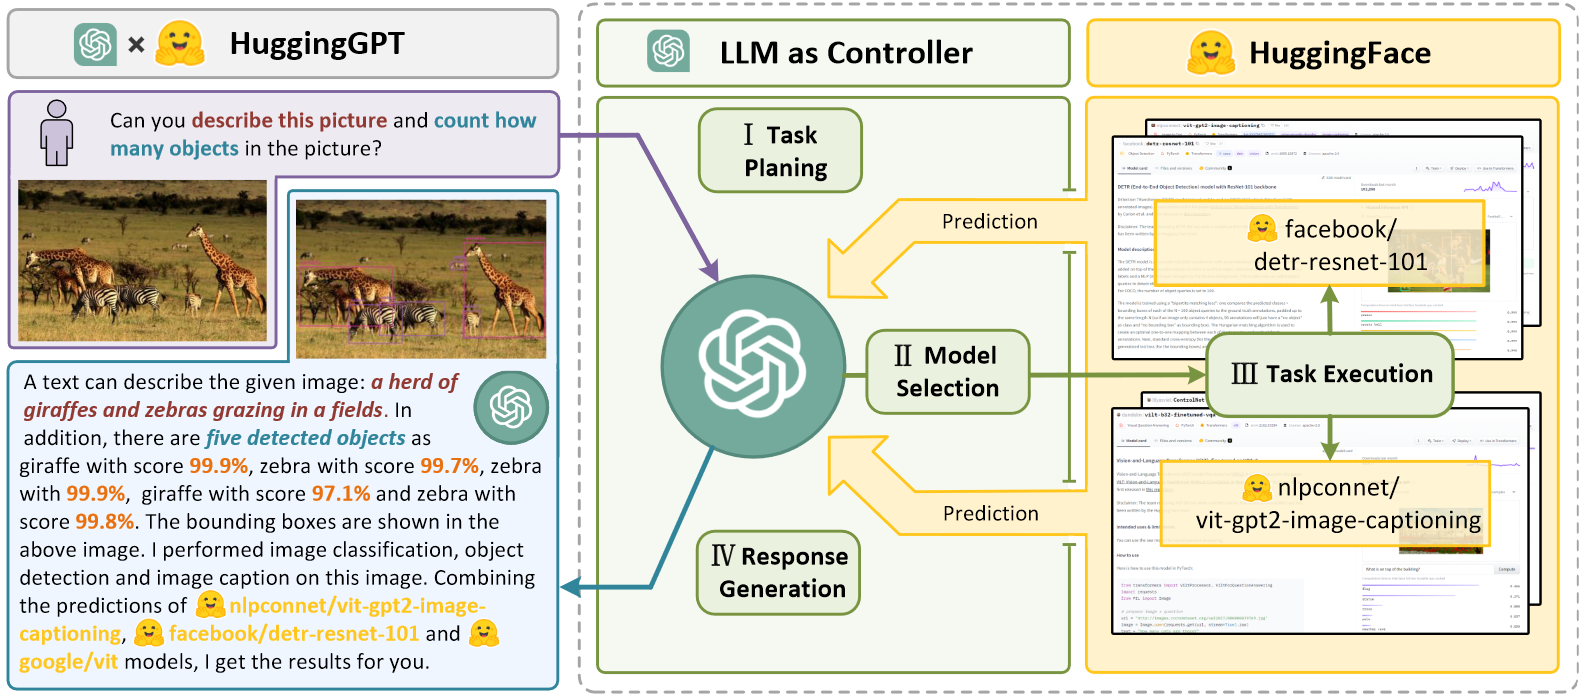
\includegraphics[width=1.0\linewidth]{HuggingGPT.png}
	\caption{HuggingGPT \cite{shen_hugginggpt_2023}}
	\label{fig:hugginggpt}
\end{figure}
Task planning: user request to intention and decompose into subtasks
model selection: Hugging Face model based ion their description
task execution: invoke and execute model, results to LLM
response generation: integrate all models answers
translate task into intention and decompose into several ML subtasks, parse into task list, determine
task format: \verb|[{"task": task, "id", task_id, "dep": dependency_task_ids, "args": {"text": text, "image": URL, "audio": URL, "video": URL}}]|
dep: dependency with id of previous task
Prompt asks the LLM to generate task list in specific format and provides examples of task lists (demonstrations) to queries execution order, resource dependencies among tasks
JSON format for all formal specifications, templates
global planning, not iterative
iterative: more queries, danger of ending in endless loop
globally: relies on correctness and executability of each step
clear pipeline with 4 steps
par/excerpt from the planning prompt:
\begin{verbatim}
	#1 Task Planning Stage - The AI assistant performs task parsing on user input, generating a list of tasks with the following format: [{"task": task, "id", task_id, "dep": dependency_task_ids, "args": {"text": text, "image": URL, "audio": URL, "video": URL}}]. The "dep" field denotes the id of the previous task which generates a new resource upon which the current task relies. ... The task must be selected from the following options: {{ Available Task List }}. Please note that there exists a logical connections and order between the tasks.... Here are several cases for your reference: {{ Demonstrations }}. To assist with task planning, the chat history is available as {{ Chat Logs }}, ...
\end{verbatim}
type of task, id for dependencies, dep dependencies/prerequisite tasks, args: text/image/audio resources for task execution
example demonstration:
\begin{verbatim}
	Can you tell me how many objects in e1.jpg? [{"task": "object-detection", "id": 0, "dep": [-1], "args": {"im age": "e1.jpg" }}]
\end{verbatim}
GPT models: gpt-3.5-turbo, text-davinci-003 and gpt-4 variants, OpenAI API
GPT-3.5 showed better planning capabilities (eg dependencies of tasks) than Alpaca-7b and Vicuna-7b
stable outputs: decoding temperature to 0
JSON format: set the logit\_bias to 0.2 on the format constraints (e.g., “{” and “}”)
needs reliability of LLM, multiple interactions with LLM, limit of maximum token length (eg to incorporate all model descriptions), instability (reliability of LLMS)

TODO ADD: Chameleon: Plug-and-Play Compositional Reasoning with Large Language Models
which is really similar to HugginGPT! \cite{lu_chameleon_2023}


\cite{gao_efficient_2024} Efficient Tool Use with Chain-of-Abstraction Reasoning, Offline planning, see also actions
Chain-of-Abstraction CoA/planning with abstract chains: decode reasoning chains with placeholders, then call domain tools: reify reasoning chain/fill in specific knowledge, eg use calculator on placeholder variables
LLM fine-tuned to generate abstract multi-step reasoning chain with placeholders on a user question. Call external tools to reify step with domain specific knowledge and fill in placeholders
generate chain of reasoning once. Then add knowledge (other approaches rather interleaving)
experiments show seems especially beneficial with long reasoning chains

\paragraph{Iterative Task Generation}

TODO INTRO: 
recursive prompting, re-prompting 
closed-loop systems 
environment feedback, monitoring, adjustment/adaptation/refine 
flexibility 
when to update plan? after each action execution and receive environment feedback? 
iterative, thought-action-observation interweaving (e.g. ReAct) 
also called autoregressive chaining? 
add LLM generated output to next input/to context window

can either change only one single action based on the feedback, refinement, integrate information for better action grounding, then generate future actions based on this updated context
or refining the entire plan (see next section), potentially changing up to all future actions, env feedback directly used to revise entire plan

\cite{ahn_as_2022} 16.08.2022 SayCan -see also tool availability via descriptions
LLM not physically grounded in environment, cannot observe physical consequences of actions
LLM: high-level semantic knowledge, complex, temporally extended goals/instructions
robot: "hands and eyes", low-level skills, 
combine: need feasible and contextually appropriate actions
subtask decomposition: only reasonable if: context knowledge about robot capabilities, current state and information about environment
LLM interpret instruction + likelihood evaluate how a skill can help progress towards goal + affordance function) how likely it will succeed: LLM "aware" of capabilities + explainable reasoning/choosing of steps/actions
Affordance functions: learned by RL
grounding via affordances: leads to doubled performance on robotic tasks
set of skills and affordance function for probability of completing skill successfully from state s
LLM should propose optimal skill
multiply LLM probability of skill being useful for high-level instruction with affordance function of successful execution probability
break down high-level instruction into sequence of available low-level skills
set of skills, skill: policy (e.g. learned), value function (TD/RL), short language description (e.g.g "pick up the can")
algorithm SayCan, TODO: as algorithm not image 
\begin{figure}[h]
	\centering
	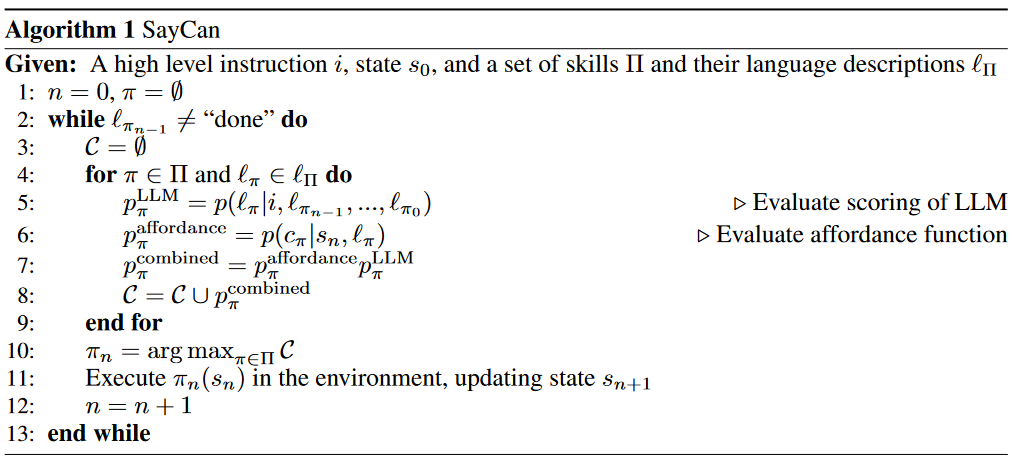
\includegraphics[width=0.8\linewidth]{SayCanAlgorithm}
	\caption{SayCan algorithm \cite{ahn_as_2022}}
	\label{fig:saycanalgorithm}
\end{figure}
condition policies on language: pre-trained large sentence encoder language model. generate embeddings by passing in Text descriptions of each skill -  this is input to policy and value function
LLMs: PaLM 540B
can additionally add CoT reasoning to provide an explanation of a task for reasoning
Iterative planning:
\begin{figure}[h]
	\centering
	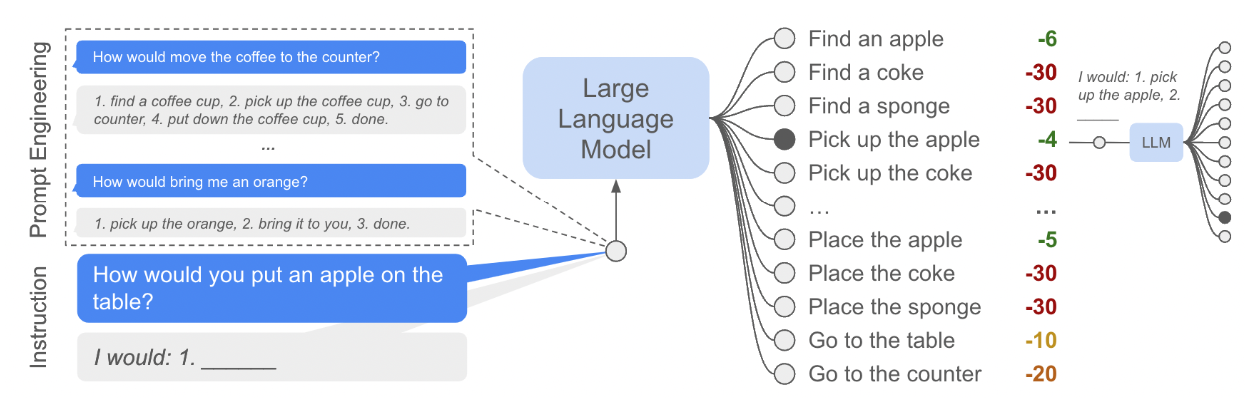
\includegraphics[width=0.85\linewidth]{SayCanScoringLLM.png}
	\caption{SayCan Scoring LLM, prompt-engineered examples, output: probability of each skill being selected, interetively plan next step: add selected skill to query and query LLM again \cite{ahn_as_2022}}
	\label{fig:saycanscoringLLM}
\end{figure}
prompt engineering:
used 17 examples. Already with 4 provided examples food
used explicit numbers between steps improved performance, separate line for each step ("\\n")
spelling errors problematic
demo prompt is structured like a dialogue
example (1):
\begin{verbatim}
	Robot: Hi there, I’m a robot operating in an office kitchen. 
	Robot: You can ask me to do various tasks and I’ll tell you the sequence of actions I would do to accomplish your task.
	Human: How would you move the water bottle from the table to the counter? Robot: 1. find a water bottle, 2. pick up the water bottle, 3. go to the counter, 4. put down the water bottle, 5. done.
\end{verbatim}
including CoT example: 
\begin{verbatim}
	Robot: Hi there, I’m a robot operating in an office kitchen. 
	You can ask me to do various tasks and I’ll tell you the sequence of actions I would do to accomplish your task. 
	The following objects are in the scene: 7up, apple, tea, multigrain chips, kettle chips, jalapeno chips, rice chips, coke, grapefruit soda, pepsi, redbull, energy bar, lime soda, sponge, and water bottle. 
	The following locations are in the scene: close counter, far counter, table, you, trash, bowl.
	Human: Bring me something that isn’t a fruit 
	Explanation: The user has asked for something food that isn’t an fruit, I will bring an energy bar. 
	Robot: 1. find an energy bar, 2. pick up the energy bar, 3. bring it to you, 4. put down the energy bar, 5. done.
\end{verbatim}


ReAct: Thought - Action - Observation (=outcome of action)
\url{https://www.promptingguide.ai/techniques/react}
ReAct \cite{yao_react_2023} {ReAct}: {Synergizing} {Reasoning} and {Acting} in {Language} {Models}
Thought-action-observation: combine reasoning and action
iterative executor, thoughts+actions, can lead to large history
before: rather either reasoning (CoT) or acting, here: together/interleaved
"generate both reasoning traces and task-specific actions in an interleaved manner"
track and update action plans, handle exceptions
interface with environment and gather additional information
help overcome hallucination and error propagation in CoT
CoT not grounded in external world, CoT internal own model
combine reasoning and acting
dynamic reasoning, create and adjust high-level plans, interact with environement eg Wikipedia, additional information
prompt-based paradigm
ReAct in few-shot learning setup
interaction setup: 
"At time step $t$, an agent receives an observation $o_t \in O$ from the environment and takes an action $a_t \in A$ following some policy $\pi(a_t | c_t)$, where $c_t = (o_1, a_1, \ldots, o_{t-1}, a_{t-1}, o_t)$ is the context to the agent. Learning a policy is challenging when the mapping $c_t \rightarrow a_t$ is highly implicit and requires extensive computation."
idea: augment action space by language space, action in language space: thought, reasoning trace, thought no effect in environment but reasons and comprises information, reasoning over current context, and updates current context
$A = A \cup L$, where $L$ is the space of language. An action $\hat{a}_t \in L$, $c_{t+1} = (c_t, \hat{a}_t)$
PaLM-540B, GPT-3(text-davinci-002, greedy decoding) 
in-context examples: "human trajectory of actions, thoughts, and environment observations to solve a task instance"
trajectory: multiple thought-action-observation steps
thoughts not need t occur at every step
simple design, use six demonstrations, reasoning process more human interpretable
less hallucinations
BUT: special reasoning error with ReAct, repetitively generating previous thoughts and actions, and in general increased error rate, successfully retrieving information via search is critical
human-in-the-loop possible!
can remove some hallucination and add hints
Part of the demonstration, as example:
\begin{verbatim}
	Question	What is the elevation range for the area that the eastern sector of the Colorado orogeny extends into? 
	Thought 1	I need to search Colorado orogeny, find the area that the eastern sector of the Colorado orogeny extends into, then find the elevation range of the area. 
	Action 1	Search[Colorado orogeny] 
	Observation 1	The Colorado orogeny was an episode of mountain building (an orogeny) in Colorado and surrounding areas. 
	Thought 2	It does not mention the eastern sector. So I need to look up eastern sector. Action 2	Lookup[eastern sector]
	...
	Action 5	Finish[1,800 to 7,000 ft]
\end{verbatim}


\cite{noauthor_babyagi_nodate} \cite{nakajima_babybeeagi_2023}
intelligent task manager
infinite loop
pull task from list, execute, enhance outcomes, generate new tasks based on initial objective and outcome of previous task
Pulls the first task from the task list.
Sends the task to the execution agent, which uses OpenAI's API to complete the task based on the context.
Enriches the result and stores it in Chroma/Weaviate.
Creates new tasks and reprioritizes the task list based on the objective and the result of the previous task.
\begin{figure}[h]
	\centering
	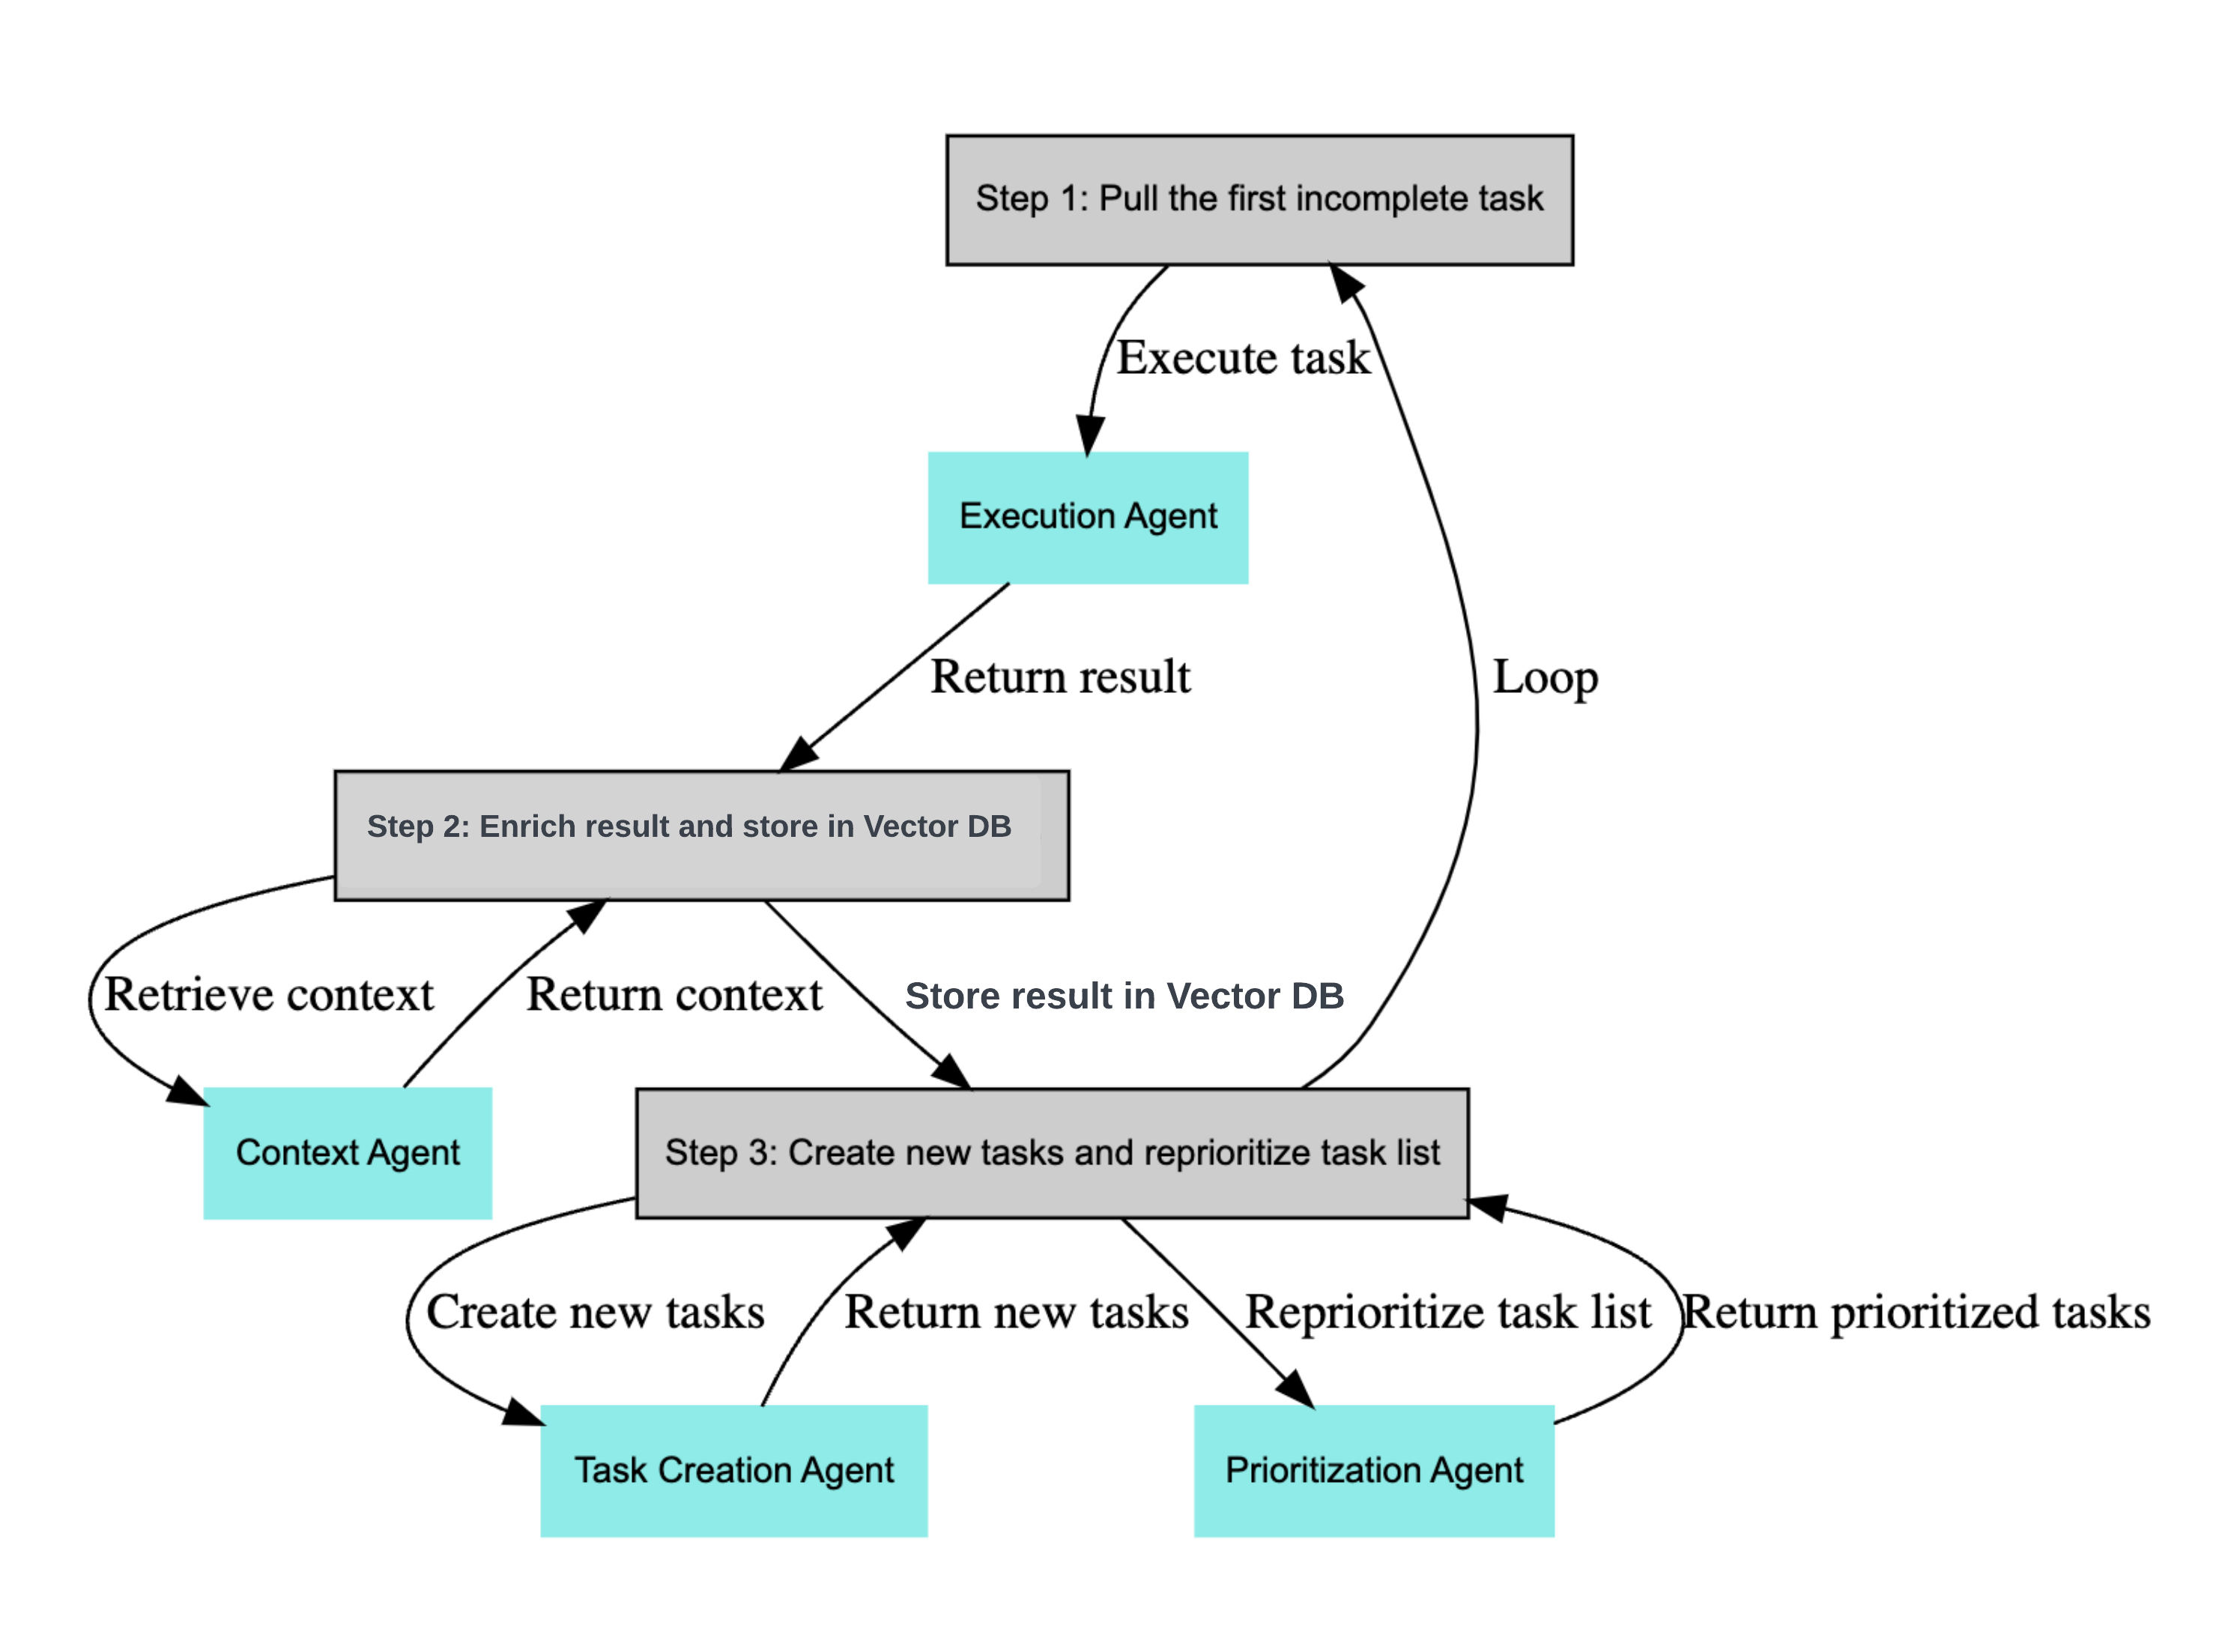
\includegraphics[width=0.75\linewidth]{BabyAGIFlow}
	\caption{BabyAGI \cite{noauthor_babyagi_nodate}}
	\label{fig:babyagiflow}
\end{figure}
BabyBeeAGI: enhancements/versions: dependent tasks, tools like web search
\begin{figure}[h]
	\centering
	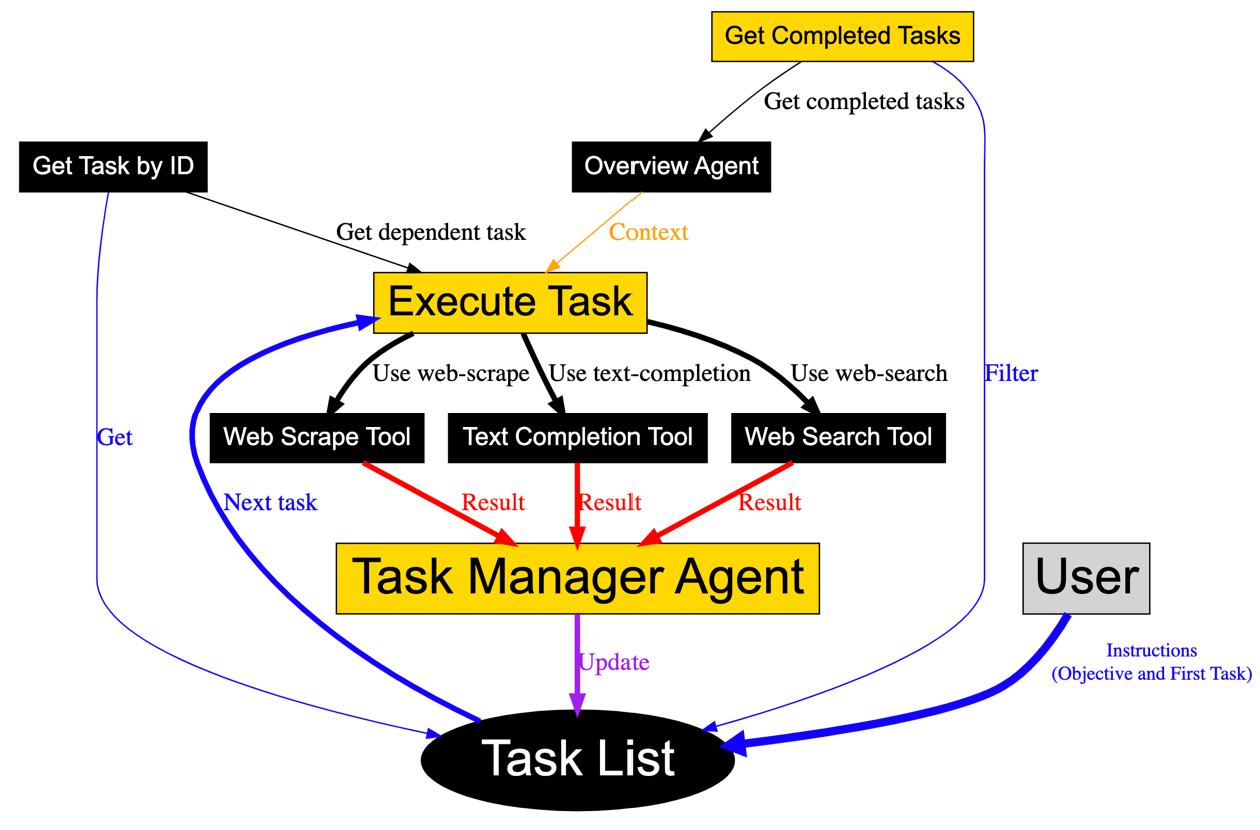
\includegraphics[width=0.75\linewidth]{BabyBeeAGIFlow}
	\caption{BabyBeeAGI \cite{nakajima_babybeeagi_2023}}
	\label{fig:babyagiflow}
\end{figure}





\cite{wang_voyager_2023} 19.10.2023 VOYAGER: An Open-Ended Embodied Agent with Large Language Models
lifelong learning agent in Minecraft
GPT-4
develops skills: temporally extended, interpretable, compositional
three key components:  automatic curriculum that maximizes exploration, skill library, iterative prompting mechanism
1) an automatic curriculum that maximizes exploration, 
description to program, generated by GPT 3.5
text-embedding-ada-002 [51] API for text embedding
query library: GPT-3.5 uses pretrained knowledge to add context to a task, then embedding of task used to retrieve relevant skills from library
Skill /code generation input to prompt: Guidelines for code generation, APIs and relevant skills from library, generated code from last round with feedback, agent current state in game, CoT prompting for reasoning before code generation
3) a new iterative prompting mechanism that incorporates environment feedback, execution errors, and self-verification for program improvement.
code as the action space instead of low-level motor commands 8can represent then temporally extended and compositional actions)
-execute a generated program  and obtain observations from minecraft environment or error trace of code interpreter
- use for GPT-4 prompt feedback for code refinement
- refine until self-verification module confirms task completion (then program added to skill library), GPT-4 agent: current state+task, let check whether program achieves task
Skill library and feedbacks significant in ablation studies, also very huge difference to using GPT-3.5 for code generation, self-verification most important feedback type
is possible to use feedback from humans instead of self-verification module
high costs for GPT-4 calls

\cite{du_anytool_2024} AnyTool: Self-Reflective, Hierarchical Agents for Large-Scale API Calls
not directly planning, see actions tools
just assumption
16,000 APIs from Rapid API: subset of the APIs can resolve the queries

Add ChatCot? \cite{chen_chatcot_2023}

\paragraph{Online Replanning}
plan with online re-planning,
online planning: integrate planner in action loop of agent, monior execution of plan and revise planning when needed

INTRO- Why beneficial:
Touvron et al., 2023? correlation between subtasks and original task?
errors in single steps lead to overall failure without replanning
iterative/interleaved: environment feedback: better fault tolerance, can lead to longer more complicated trajectories, deviating, repetitions

Inner Monologue: ADD? employs replanning, but the actual process of replanning when receiving feedback is not mentioned! \cite{huang_inner_2022}

\cite{sun_adaplanner_2023-1} 26.05.2023 LLM has two roles: planner and refiner
generates initial planning policy for solving the task
observation after each action, may modify the actions according to the feedback 
in beginning high level planning policy generating entire plan, later action-generation policy o a given plan
ALFWorld tzext based virtual household environment, MiniWoB++ simulation environment of computer tasks (web tasks)
see  also Environment feedback REFERENCE
\begin{figure}[h]
	\centering
	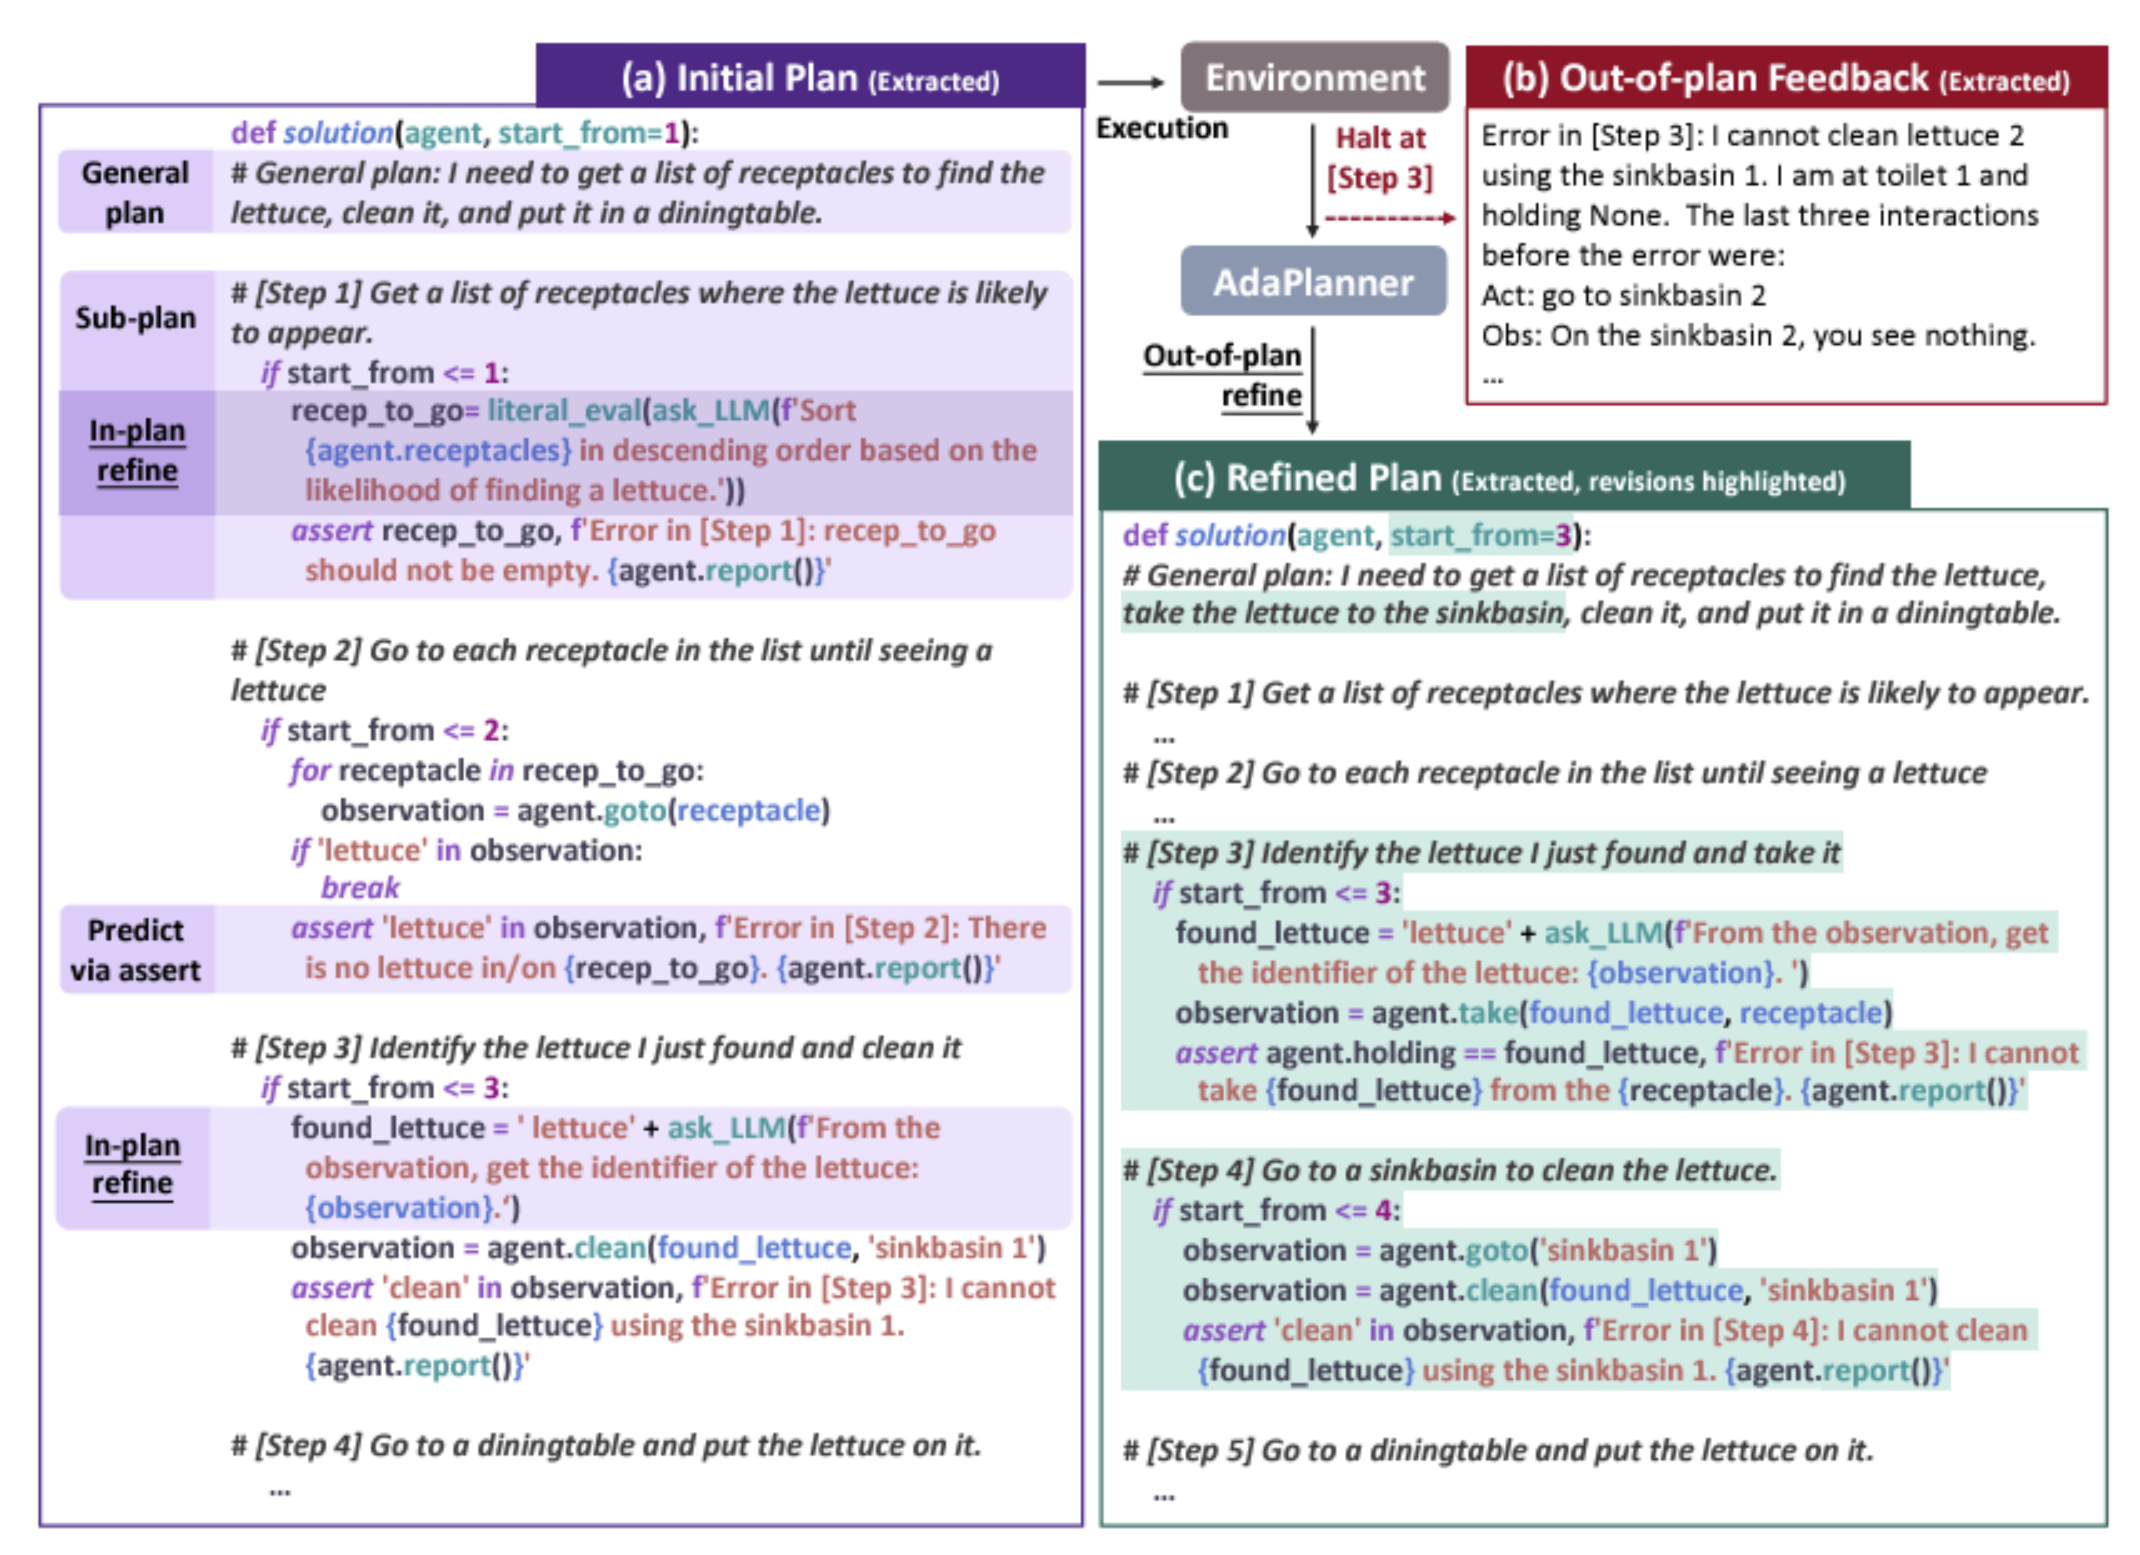
\includegraphics[width=1.0\linewidth]{AdaPlannerRefinementFlow.png}
	\caption{AdaPlanner ...\cite{sun_adaplanner_2023-1} p.5}
	\label{fig:llmagentoverview}
\end{figure}
in-plan feedback: use information from observation to adapt context knowledge for tasks
out-of-plan-feedback: generate revised plan from current step onwards
initially provide one exper sample of solution per task
part of the refinement prompt:
\begin{verbatim}
# Task: <task> You have generated code of solution() to solve the task: <solution_func> 

However, you executed the solution() function and get an error message: [Error message] <feedback> 

Let's think step by step. You must output the revised solution function based on the error message. You must only complete the revised solution function without any other words.
\end{verbatim}

ProgPrompt: Replan = rewrite the program code \cite{singh_progprompt_2023} 28.08.2023

recursive decomposition/hierarchy
\cite{prasad_adapt_2023} 08.11.2023 recursive subtask decomposition. decomposition as needed: if task is not executable
As-Needed Decomposition and Planning for complex Tasks (ADAPT), a recursive algorithm that further decomposes sub-tasks when necessary,
if task cannot be executed it is assumed to bee too complex and is then decomposed into subplan
improved success rate compared to previous approaches with GPT-3.5
planner module and executor module
controller ADAPT:
two options: try to execute input task directly, else call planner to decompose the task, 
then recursively call this/controller
theoretically always a complete plan, only at different hierarchy levels?
needs termination criterium because of recursiveness 
only one "round" of decomposing task like in ReAct? may ot be sufficient, for complex tasks further decomposition can increase performance, the more complex the more it can improve
planner includes AND and OR logic: linearly tasks all must, or alternatives

(nothing special)
\cite{raman_cape_2023} 22.10.2023 planning few-shot??
Planning LLM: demonstration set: high-level example task and respective plan, cosine similarity with query task, generate actions for task
step by step: append action, further autoregressive steps
corrective prompt 
whole plan? + corrective actions in case of precondition violation (re-planning)

\cite{wang_describe_2023} 29.10.2023
Interactive Planning with Large Language Models (goal: for open world tasks, long-term tasks, parallel subgoals)
DEPS: Describe, Explain, Plan and Select
initial LLM generated plan, integrate description of plan execution process, self-explanation of feedback of failures
trainable goal selector (rank parallel candidate sub-goals on estimated number of steps)
LLM-based planner with domain specific knowledge for the environments (Minecraft, ALFWorld, Tabletop environments)
challenges: sub-task dependencies and state-dependent task feasibility
controller fails to complete subgoal: descriptor that summarizes current situation - to LLM planner for adjusting plan, LLM as explainer to locate errors in previous plan, planner then refines plan based on descriptor and explainer
planner: decomposes high level goal into short-horizon subgoals. goal-preconditioned policy generates action based on current state and sub-goal
LLM as zero-shot planner: goal/task, decompose into sequence of subgoals as initial plan
action: controller, execute the provided sub-goals sequentially through a goal-conditioned policy
action fails: descriptor: summary of current state end execution outcome of most recent goal. LLM: explainer/self-explanation to locate error, re-plan current task/generate revised plan (to original)
prompt-template: python like code
not only environment feedback that execution failed, but "describe, explain and plan"
structured prompt: goals with preconditions and effects, interactive dialogue format
descriptor for feedback: human feedback/human description or pre-trained vision-language model, or returned information from (simulation) environment/available symbolic information
explainer: few-shot CoT
LLMS: code-davinci-02 text-davinci-03 gpt-3.5-turbo
LLM planner: Codex, ChatGPT,GPT3, GPT-4 as planners, LLaMA2 + own fine-tuned LLaMA2
maximum token limits: limits maximum number of re-planning rounds
assumption: pre-trained LLM already cover /dad exposure to minecraft-related corpus
prompt for explainer explainer:
\begin{verbatim}
	Here are some actions that the agent fails to perform in Minecraft. Please give the explanation of action execution failure according to the current inventory information of the agent. 
	
	### Failed Action: mine({’iron_ore’:1}, null); # step 5: mine 1 iron_ore without tool Current Inventory: null Explanation: Because mining iron_ore needs to use the tool stone_pickaxe, but my inventory does not have stone_pickaxe. So I need to craft stone_pickaxe first.
\end{verbatim}
Goal parser: pre-defined controller skill set. KKM Sentence-Bert model to select most similar skill to current goal
Example of DEPS full prompt process:
\begin{verbatim}
	User: How to obtain 1 stone_sword in Minecraft step-by-step? 
	Planner: The code for obtaining stone_sword is as follows: 
	def obtain_1_stone_sword(inventory = {}): 
	mine({’log’:3}, null); # step 1: mine 3 log without tool 
	craft({’planks’:12}, {’log’:3}, null); # step 2: craft 12 planks from 3 log 
	craft({’stick’:4}, {’planks’:2}, null); # step 3: craft 4 stick from 2 planks 
	mine({’cobblestone’:2}, null); # step 4: mine 2 cobblestone without tool 
	craft({’stone_sword’:1}, {’cobblestone’:2, ’stick’:1}, ’crafting_table’); # step 5: craft 1 stone_sword from 2 cobblestone and 1 stick, on crafting_table 
	return ’stone_sword’ 
	
	Descriptor: I succeed on step 1, 2, 3, but I fail on step 4 "mine({’cobblestone’:2}, null);". My inventory now has 10 planks, 4 stick. 
	Explainer: Because mining cobblestone needs to use the tool wooden_pickaxe. 
	User: Please fix the above errors and replan the task "obtain 1 stone_sword". 
	RePlanner: The code for crafting stone_sword is as bellows: def obtain_1_stone_sword(inventory = {’planks’:10, ’stick’:4}):
\end{verbatim}
action: controller, execute the provided sub-goals sequentially through a goal-conditioned policy for minecraft



\FloatBarrier
\section{Action Matching}
DRAFT: ONLY NOTES

TODO INTRO

Action execution: 
agents decisions/steps/tasks to concrete action executions 
acting in environment 
some actions could CHANGE the environment! 
diverse: internet or special page search (wiki), code interpreter, database,... external models, query
workflow: how to interact with tools and get the results/observations/information
also e.g RAG/RAG pipeline as a tool
wording: TALM: tool augmented language models?
LLM as action executor, interaction with environment by LLM executor generated actions, LLM can et list of possible actions/skills and/or demonstrations 
Can query memory before execution to get additional information

Different types of actions \cite{wang_survey_2023} perspective of action goal/objectives of actions:
task completion, communication, environment exploration
action space perspective: external tools, "internal" knowledge of LLM
internal: planning step/decomposition, conversation

TODO some of the notes from \cite{ghallab_automated_2016} "Automated planning and acting" for intro

%\cite{ghallab_automated_2016} Automated planning and acting
%deliberation needed: computer system autonomously performing in diverse environment or diverse tasks
%acting: action of an agent
%deliberately: motivated by intended objective, deliberation: deciding for action and how to perform to reach objective
%This needs a reasoning process (eg how to perform an action and what will be the expected result)
%reasoning: predictive model of agents environment/simulative capabilities
%actor (consider intelligent agent but with focus on acting functions)
%deliberation needed: autonomy + diversity in tasks and environments
%GhallabNauTraverso-Actor.png Figure 1.1: Conceptual view of an actor (a); its restriction to planning and
%acting (b).
%"To choose and execute commands that
%ultimately achieve its objectives, the actor needs to perform a number of
%deliberation functions. For example, the actor must commit to intermediate
%goals, plan for those goals, refine each planned action into commands, react to events, monitor its activities to compare the predicted and observed
%changes, and decide whether recovery actions are needed. These deliberation
%functions are depicted in Figure 1.1(b) as two main functions: planning and
%acting. The acting function is in charge of refining actions into commands,
%reacting to events, and monitoring."
%deliberation can be: multiple lebels of abstraction in deliberative acting: refine abstract actions into more concrete ones when needed
%"two important principles of deliberation: hierarchical organization and continual online processing"
%actions may need further refinement and planning
%"This is done online and may require different representations,
%tools, and techniques from the ones that generated the task. A hierarchized deliberation process is not intended solely to reduce the search
%complexity of offline plan synthesis. It is needed mainly to address
%the heterogeneous nature of the actions about which the actor is deliberating, and the corresponding heterogeneous representations and
%models that such deliberations require."
%"Continual online deliberation. Only in exceptional circumstances will
%the actor do all of its deliberation offline before executing any of its
%planned actions. Instead, the actor generally deliberates at runtime
%about how to carry out the tasks it is currently performing."
%often limited predictive models
%cost of exentsive modeling vs cost of minor mistakes and retrials
%needs refinement and monioring of actions, reaction to events, extends/updates/repairs to a plan
%Deliberation assumptions: classification of environment
%Dynamics of environment: static/dynamic, discrete/continuous/hybrid, observability, uncertainty, time and concurrency
%Models of actions:
%descriptive models: "describe which state or set of possible states may result from performing an action or command. They are used by the actor to reason about
%what actions may achieve its objectives" - higher level of deliberation, simplifications
%operational models: know how, how to perfrorm an actins/which commands to execute - must take int account diverse circumstances and exogenous events
%states described with state variables, data structures and state representations, can be heirarchy/abstract
%"planning is to synthesize an organized set of actions
%to carry out some activity"
%"Acting involves deciding how to perform the chosen actions"... "while reacting to the context in which the
%activity takes place. "
%"Seeking a complete plan before
%starting to act is not always feasible, and not always needed. It is feasible
%when the environment is predictable and well modeled" or when actions have high cost or risk or are not reversible
%online planning: integrate planner in action loop of agent, monior execution of plan and revise planning when needed
%possibil use receding horizon planning
%--LATER: see chapter 3 Refinement methods, can use operational models of actions which weakons assumptions: can work on dynamic non-static environments, imperfect information, overlapping(time) actrions, nondeterminism, hierarchically organized actors and discrete and cintinuous variables --as opposed to the classical planning!
%in our domain, environment probably seen as nondeterministic because just cannot foresee ancode all possibel outcomes??  tjhen plan not sufficient as sequence of actions but might need a conditional plan
%possible: use online planning
%maybe need the notions of weak, striong cyclic and strong soltios (or solution, unsafe, safe, cyclic safe, acyclic safe)
%(symbolic model checking probaly not possible: would still need to represent all possible following states - but they may be unknown!!)
%open world assumption
%planning with information gathering (see chapter 7!) can e.g.g rely on OWL (web ontology language) where facts can be true, false or unknown
%monitoring
%(learning operational models?? then rather use learned operational models! eg to produce SQL queries!)


\subsection{Action/Tool Selection}
DRAFT: ONLY NOTES

select action (most often: tool) among diverse options
tool definition prompt examples

TOOLS PREDEFINED PER EXPERIMENT
\cite{gao_efficient_2024} Efficient Tool Use with Chain-of-Abstraction Reasoning, see also offline planning
grounding to real-world knowledge needed: can be achieved via tool calls
need for holistic and efficient tool usage planning in multi-step reasoning
Chain-of-Abstraction CoA/planning with abstract chains: decode reasoning chains with placeholders, then call domain tools: reify reasoning chain/fill in specific knowledge, eg use calculator on placeholder variables
learn general reasoning strategy, parallel decoding and external tool calling (possibly less inference delay)
LLM fine-tuned to generate abstract multi-step reasoning chain with placeholders on a user question. Call external tools to reify step with domain specific knowledge and fill in placeholders
generate chain of reasoning once. Then add knowledge (other approaches rather interleaving)
experiments show seems especially beneficial with long reasoning chains

argue: not practical, because as soon as there are several tools, tools must be chosen!

\subsubsection{Reasoning on a List of Action/Tool Descriptions}
Tool Availability via Descriptions

\cite{shen_hugginggpt_2023} HuggingGPT: Solving AI Tasks with ChatGPT and its Friends in Hugging Face
AI tasks, different domains, modalities
models for specific tasks
how to handle complicated task?
LLM as controller for different AI models
ChatGPT
LLM: task planning, 
select model (according to function description in HuggingFace) to execute subtask
summarize response
complex AI/ML tasks consisting of multiple subtasks, requiring different specialized models, expert models (e.g. finetuned to specific tasks)
how to connect LLM and expert models? via language, language as interface
needed: high-quality model descriptions
model selection: Hugging Face model based ion their description
task execution: invoke and execute model, results to LLM
response generation: integrate all models answers
select model best for task
execute task, model via endpoint
summarize all results
JSON format for all formal specifications, templates
prompt to select a model (tool)
\begin{verbatim}
	#2 Model Selection Stage - Given the user request and the call command, the AI assistant helps the user to select a suitable model from a list of models to process the user request. The AI assistant merely outputs the model id of the most appropriate model. The output must be in a strict JSON format: {"id": "id", "reason": "your detail reason for the choice"}. We have a list of models for you to choose from {{ Candidate Models }}. Please select one model from the list.
\end{verbatim}
candidate model (tools) descriptions
\begin{verbatim}
	{"model_id": model id #1, "metadata": meta-info #1, "description": description of model #1}
\end{verbatim}
stable outputs: decoding temperature to 0
JSON format: set the logit\_bias to 0.2 on the format constraints (e.g., “{” and “}”)
needs reliability of LLM, multiple interactions with LLM, limit of maximum token length (eg to incorporate all model descriptions), instability (reliability of LLMS)
\cite{shen_hugginggpt_2023} HuggingGPT, Multi path but linearization (several prerequisite dependencies)
task format: \verb|[{"task": task, "id", task_id, "dep": dependency_task_ids, "args": {"text": text, "image": URL, "audio": URL, "video": URL}}]|
dep: dependency with id of previous task
Prompt asks the LLM to generate task list in specific format and provides examples of task lists (demonstrations) to queries
tasks can depend on several previous/prerequisite dependencies on resources produced by previous tasks


%TODO also/more to Action Instantiation?
\cite{huang_language_2022} Language Models as Zero-Shot Planners: Extracting Actionable Knowledge for Embodied Agents - only aspect of finding corresponding admissible action
everyday household tasks
plans which are not directly executable in environment - linguistic ambiguity or no fitting admissible action
they: "enumerate all admissible actions and map the model’s output phrases to the most semantically-similar admissible action (we use similarity measure between sentence embeddings produced by a RoBERTa model [27] in this work, but other choices are possible)"
+ generate actions by conditioning past actions made admissible by similarity measure...
translate each step into admissible action via another pre-trained masked LLM
then append generated action to tompz and then generate remaining steps
when beneficial: need special format/structure of action, mapping of actions and objects in environment, lexical ambiguity
"to embed the output action phrase and environment actions, we use a BERT-style LM [10, 27] pre-trained with Sentence-BERT [41] objective, to which we refer as Translation LM"
after each step translation because better for guaranteeing achievability of each step
interleave plan generation and action translation
results in far more executable and correct plans (at least in robotic environment)
interestingly, depending on LLM used for planning (CODEX 12B or GPT-3 175B) different translation LMs perform better: either Sentence RoBERTa (large) or Sentence Bert (base)

\cite{ouyang_autoplan_2023}
no in-context demonstrations (for actual rules in environment)
instead list of possible actions, trial and error if can be applied
action prompts for Hotpot QA:
\begin{verbatim}
	Valid action formats are as follows: 
	search[entity] 
	lookup[keyword] 
	finish[answer] 
	
	Formalize the following action strictly into the above valid action formats. If there are multiple actions, formalize the first one. 
	
	Action to formalize: {raw_action} 
	Formalized action: {formalized_action}
\end{verbatim}

\cite{raman_cape_2023} actions/skills
skill library
skills described in natural language: need to ground skills in environment. Reason about: applicability, relevance and specific state changes in environment, eg query database: which concrete database with API, specific SQL query
assumed: predefined skills with preconditions, goal description, observation and action space textual description
if precondition violation (fail to execute action because precondition violation): CAPE (Corrective Actions from Precondition Errors) -  LLM queried for corrective actions
actions with preconditions:
inspired by structured affordance models from symbolic?? planning, action preconditions: factorize states into preconditions. affordance: state components satisfied
Options framework: O(s) over state space S: set of temporally extended actions, initiation set I(o): states in which option execution is afforded, termination condition/terminal state of skill(effect) $\beta_o (s)$
current state != option initiation state - precondition error

\cite{yuan_easytool_2024} EASYTOOL: Enhancing LLM-based Agents with Concise Tool Instruction
transform tool documentation to concise description
diverse tool documentations: could be diverse, redundant, or incomplete
framework to transform tool documentation into unified and concise tool instruction for easier tool usage, offer standardized tool descriptions and functionalities for LLM-based agents
experiments: significantly reduces token consumption and can improve performance of LLM-based agents on tool utilization
tool documentation + demonstrations: consume many tokens
issues of tool documentations: inconsistency/diversity, formats, redundancy, incompleteness
approach assumed: Task planning-stage with decomposition, then tool retrieval, tool selection and tool execution
\begin{figure}[h]
	\centering
	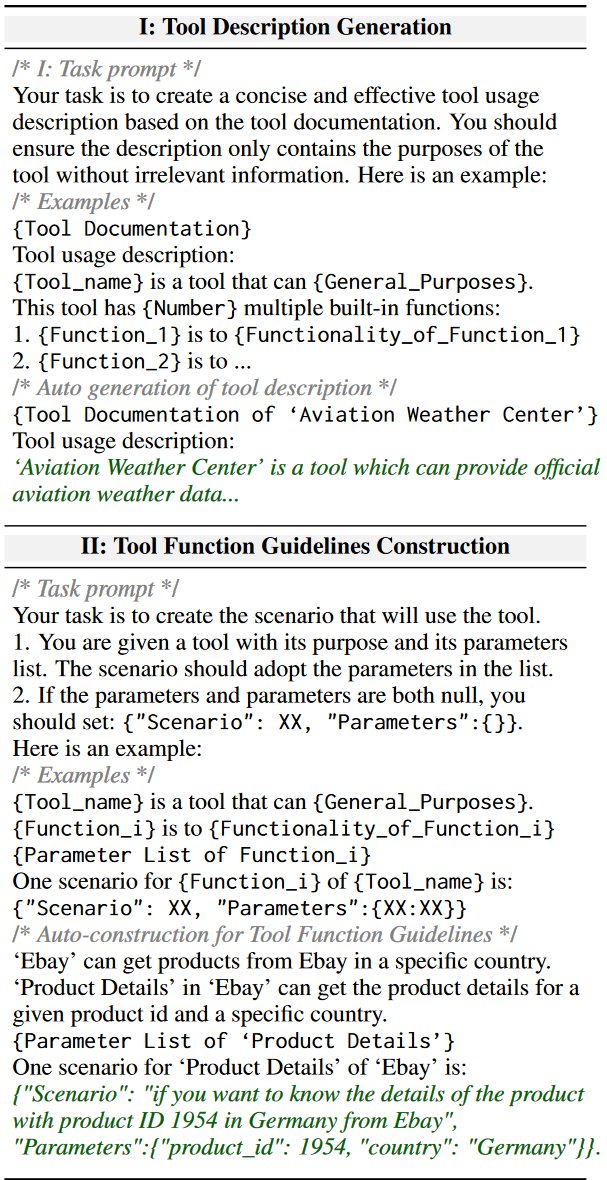
\includegraphics[width=0.55\linewidth]{EasyToolPrompts.png}
	\caption{EasyTool Prompts \cite{yuan_easytool_2024}}
	\label{fig:easytoolprompts}
\end{figure}
2 stages:
tool description generation
prompt with instruction for LLM to convert tool documentation, summarize its general purpose
include tool name, general purposes and build in functions
prompt with demonstration
tool functionality guidelines construction:
parameters of tools for execution, extract parameters from tool documentation and organize into structured output, create examples of using tool with example scenario input parameters
experiments on tool bench show greatly reduced token costs when using tooltennch,ToolBench, the token cost was reduced by 70.43\%., improves closed and open source models, also small like mistral-isntruct-7B or Vicuna-7B, huge improvement because before could solve tasks at all and then achieve hug pass/win/success rate, impressive!

\cite{du_anytool_2024} AnyTool: Self-Reflective, Hierarchical Agents for Large-Scale API Calls
16,000 APIs from Rapid API, solver: resolve user queries using set of API candidates + self-reflection: re-activation if solution impracticable
planning as tool selection
agent: gets tools per category and their description, identify most relevant API candidates for answering query
two parts: API retriever identifies API candidates, solver addresses queries using generated API-candidate pool + self-reflection
When without hierarchy in API retriever: Ablation, significant positive effects
self-reflection also significant positive effects

\cite{sun_adaplanner_2023-1} ALFWorld available actions, example of application, example of an action:
ALFWorld:
\begin{verbatim}
	# Go to a receptacle and update the agent's location. 
	# For example, 'On the countertop 1, you see a candle 1, a cloth 2, and a soapbar 1.' = goto('countertop 1') # For example, 'On the sidetable 2, you see nothing.' = goto('sidetable 2') def goto(self, receptacle): 
	...
\end{verbatim}
MiniWoB++
\begin{verbatim}
	# Action: press a key on the keyboard, the input can be one of the following: 
	# enter, space, arrow_left, arrow_right, arrow_up, arrow_down, backspace 
	# this function returns the string of the HTML code after taking the action # e.g., new_html_state = agent.press_key("enter") def press_key(self, key: str)-> str:
\end{verbatim}

+SEACRH FOR TOOL CHAIN - FITS BOTH CATEGORIES?
\cite{qin_toolllm_2023} 
"y integrating LLMs with APIs, we can greatly expand their utility and empower them to serve as efficient intermediaries between users and the vast ecosystem of applications"
ToolBench, an instruction-tuning dataset for tool use: constructed automatically using ChatGPT (gpt-3.5-turbo-16k)
16, 464 real-world RESTful APIs
prompt ChatGPT to generate diverse instructions with APIs (understand API functionality and generate possible instructions involving this API) and determine also relevant APIs for an instruction, -- (instruction, relevant API) pairs, prompt needs: description of instruction generation task, API documentations, 3 in-context examples (human written instruction generation)
and prompt ChatGPT to search for valid solution path (chain of API calls) - valid action sequence
"To let ChatGPT finish an action sequence, we define two additional functions, i.e., “Finish with Final Answer” and “Finish by Giving Up”."
depth-first search-based decision tree algorithm: evaluate multiple reasoning traces
ToolEval: automatic evaluator, ChatGPT, evaluates LLMs ability to execute an instruction within limited budgets and  compare quality and usefulness of solutions paths: high correlation with human evaluation, assessment
ToolLLaNA: finetuned LLaMA on ToolBench, recommends appropriate APIs, evaluate using ToolEval
ToolLama  "outperforms Text-Davinci-003 and Claude-2, achieves comparable performance to the “teacher model” ChatGPT, and is only slightly inferior to GPT4"
generalizability to new APIs: only needs documentation
CoT and React limitations: error propagation (propagate errors further, then trapped in faulty loop, hallucinating APIs,, +limited exploration because only one possible direction
therefore here construct decision tree)
expand decision tree, proceed along promising path or end at a node by finish by fiving up, DFS: one valid path is sufficient, less API calls to OpenAI
generate 126, 486 (instruction, solution path) pairs, which are used to train ToolLLaMA
ToolLLaMA We fine-tune LLaMA-2 7B

\subsubsection{Action/Tool Space Search?}


\cite{zhuang_toolchain_2023} TOOLCHAIN*: EFFICIENT ACTION SPACE NAVIGATION IN LARGE LANGUAGE MODELS WITH A* SEARCH
--interesting aspect: how to assign cost to actions for using A* search
series of API calls
candidate APIS: action space
tree search-based planning algorithm, action space = decision tree of API calls in a solution plan, explore acton space
A* algorithm, task specific cost function, efficient search not requiring exhaustive exploration, less steps than DFS or MCTS
task description into ordered sequence of API function calls
A* requires less function calls
needs components of cost function f(n)=g(n)+h(n)
cumulative cost g: task specific heuristic function, based on long-term memory with plans, highest longest common sub-sequence between current plan and all plans in memory and self-consistency frequency of different actions
future cost h: task.-specific heuristic function: from long term memory, relative average position score of an action appearing in the plans and Imagination score by LLM: imagined plan and further steps to estimate remaining steps/less steps
(a) Selection: Pick a frontier node with the lowest summation of cumulative cost and future cost
(b) Expansion: Expand the nodes with potential next steps.
(c) Update: Update the value functions of the newly added nodes in the search tree.
GPT-3.5-turbo and GPT-4, LLaMA-2 7B and 13B, GPT-4 better than 3.5, results worse than GPT, bit good with finetuned LLama
far more efficient than other tree search methods...but requires intricate...of the values for the cost function (because not based on simulation!)
Prompts and general execution: Like ToolBench/ based on ToolBench


\subsubsection{Action/Tool Selection Learning}

\cite{ahn_as_2022} SayCan, Tasks/Skills - see also iterative planning!
combine: need feasible and contextually appropriate actions
subtask decomposition: only reasonable if: context knowledge about robot capabilities, current state and information about environment
LLM interpret instruction + likelihood evaluate how a skill can help progress towards goal + affordance function) how likely it will succeed: LLM "aware" of capabilities + explainable reasoning/choosing of steps/actions
Affordance functions: learned by RL
grounding via affordances: leads to doubled performance on robotic tasks
set of skills and affordance function for probability of completing skill succesfully from state s
LLM should propose optimal skill
multiply LLM probability of skill being useful for high-level instruction with affordance function of successful execution probability
break down high-level instruction into sequence of available low-level skills
set of skills, skill: policy (e.g. learned), value function (TD/RL), short language nondescript (e.g.g "pick up the can")
condition policies on language: pre-trained large sentence encoder language model. generate embeddings by passing in Text descriptions of each skill -  this is input to policy and value function

\cite{schick_toolformer_2023} Toolformer: Language Models Can Teach Themselves to Use Tools
LMs can teach themselves to use external tools via simple APIs
Toolformer: model trained: decide on which API to call, when to call, which arguments to pass and how to incorporate results
self-supervised: some demonstrations for each API
then zero-shot?
learning: in-context learning, generate data set, let LLm annotate dataset with potential API calls and determine loss: which APi calls would have helped in answering the question
pretrained GPT-J model (Wang and Komatsuzaki, 2021) with 6.7B parameters
assumption: input/output of API callas are text (only then can they be inserted into text)
Augment dataset of plain text, with API call sequences, sample number of APi calls, execute, and check if responses helpful to predict future original tokens in the text
generate API calls:
\begin{figure}[h]
	\centering
	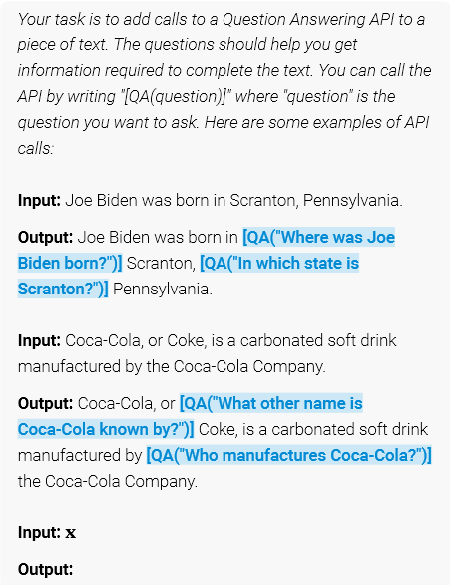
\includegraphics[width=0.5\linewidth]{ToolformerDataset.png}
	\caption{Toolformer Dataset \cite{schick_toolformer_2023}}
	\label{fig:toolformerdataset}
\end{figure}
This generated dataset is used to finetune a model
Tools: input and outputs must be text sequences + demonstrations of their use available
no tool use in interactive way, very sensitive on prompt


\subsection{Action via Code Generation}
Tool Making

\cite{wu_autogen_2023} AutoGen code execution or LLM-suggested function calls

\cite{silver_generalized_2023} Generalized Planning in PDDL Domains with Pretrained Large Language Models + see environment feedback
given: domain, training tasks
produce plans for other tasks in that domain (PDDL domains)
GPT-4
synthesize python programs
this work "only" for generalized planning, not planning! (for set of tasks, synthesize program thad produces valid plans for all the tasks)
CoT summarization and then synthesize program
automated debugging: re-prompt LLM with four types of feedback
"just two training tasks are often sufficient for strong generalization"
GPT4 should write python program that solves tasks in a planning domain
prompt: domain + training tasks , both in PDDL
python program: take task description and generate a plan
flow: 1) write summary of PDDL domain in natural language, then describe a solution strategy, then write it in python
environment feedback: errors from code execution, give error to LLLM and ask it to fix code itself
analysis: important are using GPT-4 (compared to 3.5), PDDL names, automated debugging (env exception feeedback)
produced generalized plan in python code can be inspected (maybe instead of iteratively adding new tasks) +  not many queries +  this not limited to context window size
only classical planning: deterministic, fully observable
PDDL STRIPS subset, plan then finite sequence of actions
3 stages:
write summary (need to truncate training tasks to fit into context window)
\begin{verbatim}
	Domain: [PDDL Domain] 
	Example problems: [PDDL Training Tasks] 
	Write a short summary of this domain in words.
\end{verbatim}
strategy proposal, asg for strategy
\begin{verbatim}
	There is a simple strategy for solving all problems in this domain without using search. What is that strategy?
\end{verbatim}
strategy implementation:
\begin{verbatim}
	Implement the strategy as a Python function. The code should be of the form def 
	get_plan(objects, init, goal): 
	# Your code here 
	return plan 
	where
	- objects is a set of (object name, type name) tuples
	...
\end{verbatim}
Feedback: types: python exceptions, timeout, plan syntax, plan semantics
exception:
\begin{verbatim}
	Given this task: [PDDL Training Task] 
	The code raised the following exception: 
	File "<file-name-omitted>", line 86 
	lift_at = {atom[1]: atom[2] ...}
	
	IndexError: tuple index out of range 
	Fix the code.
\end{verbatim}
plan semantics
\begin{verbatim}
	Given this task: [PDDL Training Task] 
	The code failed. It returned the following plan: 
	['(pick-up paper-1 loc-0)', ...]. 
	NOTE: (pick-up paper-0 loc-0) has an unsatisfied precondition at time 3 
	(Set (at loc-0) to true) 
	Fix the code.
\end{verbatim}

\cite{wang_executable_2024} Executable Code Actions Elicit Better LLM Agents, CodeAct
further realization: open source LLMs better with text instruction than JSON, closed source rather better with JSON format (both worse than CodeAct)

\cite{gur_real-world_2023} "acts via programming on real websites by grounding sub-instruction and HTML snippet into executable Python codes" WebAgent: Flan-U-PaLM (Chowdhery et al., 2022; Chung et al., 2022) for grounded code generation
for open-ended action spaces like in web automation
elements to interact with at a website
they: act via programming, conditional code generation,Flan-U-PaLM: executable Python program with Selenium  WebDriver,program synthesis


TODO Plan to Code execution, where to sort?
\cite{qiao_taskweaver_2023} 01.12.2023 TaskWeaver: A Code-First Agent Framework
main focus? domain-specific data analytics tasks with rich data structures? (nested lists, dictionaries, or data frames), how to handle these structures
user requests to executable code, can use user-defined plugins
dynamic plugin selection
domain specific knowledge through examples
requirements: use custom plugns, support rich data structures, stateful execution., Reasoning and acting, natural language response, code generation, domain knowledge usage, persisting artefacts
Components: Planner, Code Generator (CG), and Code Executor (CE)
Planner: break request into subtasks, execution process with self reflection, high-level plan
CG: generate code, incorporate function calls (for plugins)
plugins: function name, its description, the arguments it accepts, and what it returns
optionally: code generation examples
Code generator generates code for one step. Code executor executes the code. Result is sent back to planner and planner determines the next step (modify initial plan if outcome different to expected)
\begin{figure}[h]
	\centering
	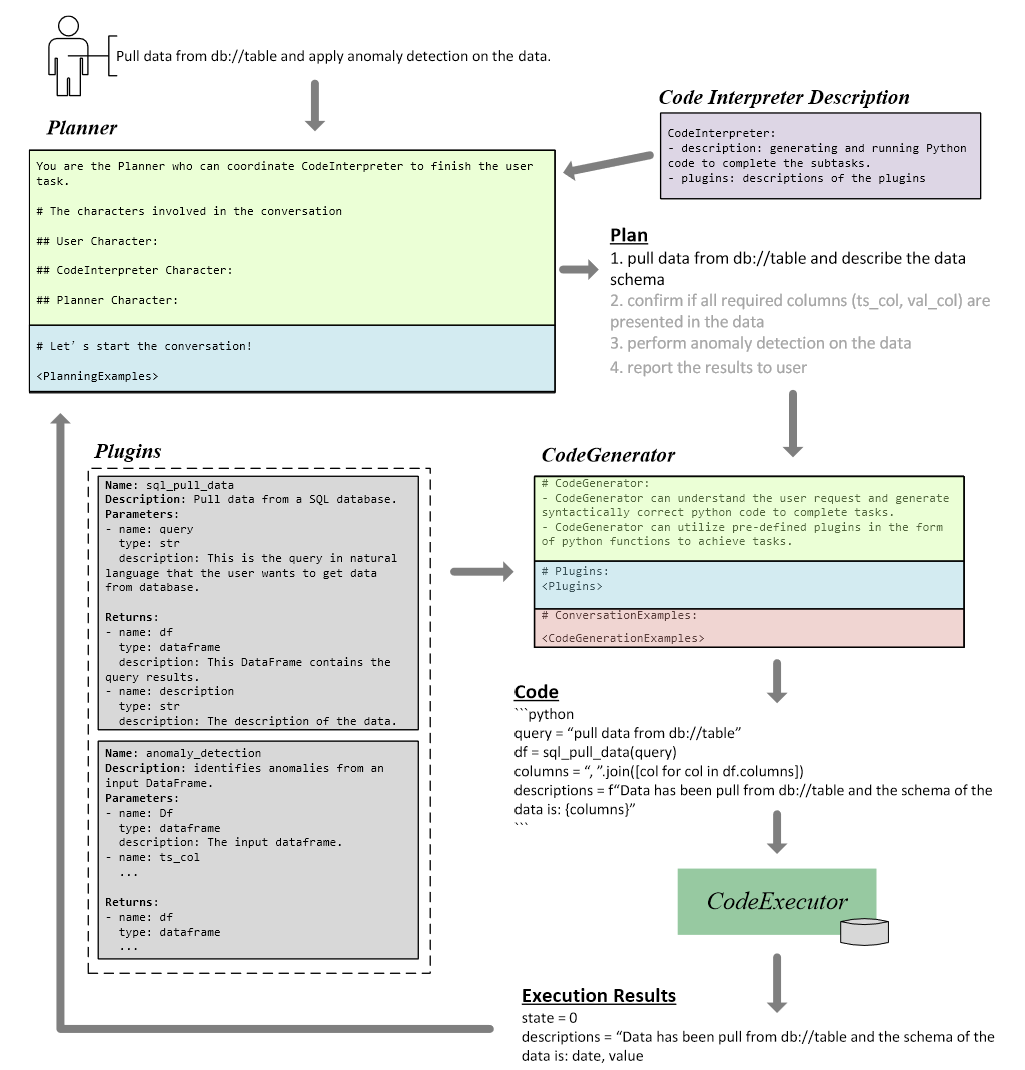
\includegraphics[width=1.0\linewidth]{TaskWeaverWorkflow.png}
	\caption{TaskWeaver Workflow \cite{qiao_taskweaver_2023}}
	\label{fig:TaskWeaverWorkflow}
\end{figure}
Task order: sequential, interactive 8need for human or LLM intervention between) or no dependency 8eg can be executed in parallel)
self reflection: if outcomes of previous steps diverge from anticipated results - modify plan
code execution error: CI can re-generate code
code feedback to planer: return code, logs, output, artefacts
optional examples: for task planning, for code generation
possible plugins- activated via function call: web API call, a software module, a customized algorithm, or a deep learning model

\cite{wang_voyager_2023} VOYAGER: An Open-Ended Embodied Agent with Large Language Models
lifelong learning agent in Minecraft
GPT-4
develops skills: temporally extended, interpretable, compositional
2) an ever-growing skill library of executable code for storing and retrieving complex behaviours, and 
store action programs that helped solve a task successfully
description to program, generated by GPT 3.5
text-embedding-ada-002 [51] API for text embedding
skill library: vector database, key= embedding vector of program description, value=program
query library: GPT-3.5 uses pretrained knowledge to add context to a task, then embedding of task used to retrieve relevant skills from library
Skill /code generation input to prompt: Guidelines for code generation, APIs and relevant skills from library, generated code from last round with feedback, agent current state in game, CoT prompting for reasoning before code generation
Skill library and feedbacks significant in ablation studies, also very huge difference to using

\cite{wang_executable_2024} Executable Code Actions Elicit Better LLM Agents, CodeAct
LLM used usually to generate JSOn or text for actions/tools, predefined tools, no composition
instead use executable python code, unified action space, execute code actions
revise actions, new actions: observations/environment interaction
finetuned from Llama2 and Mistral
\begin{figure}[h]
	\centering
	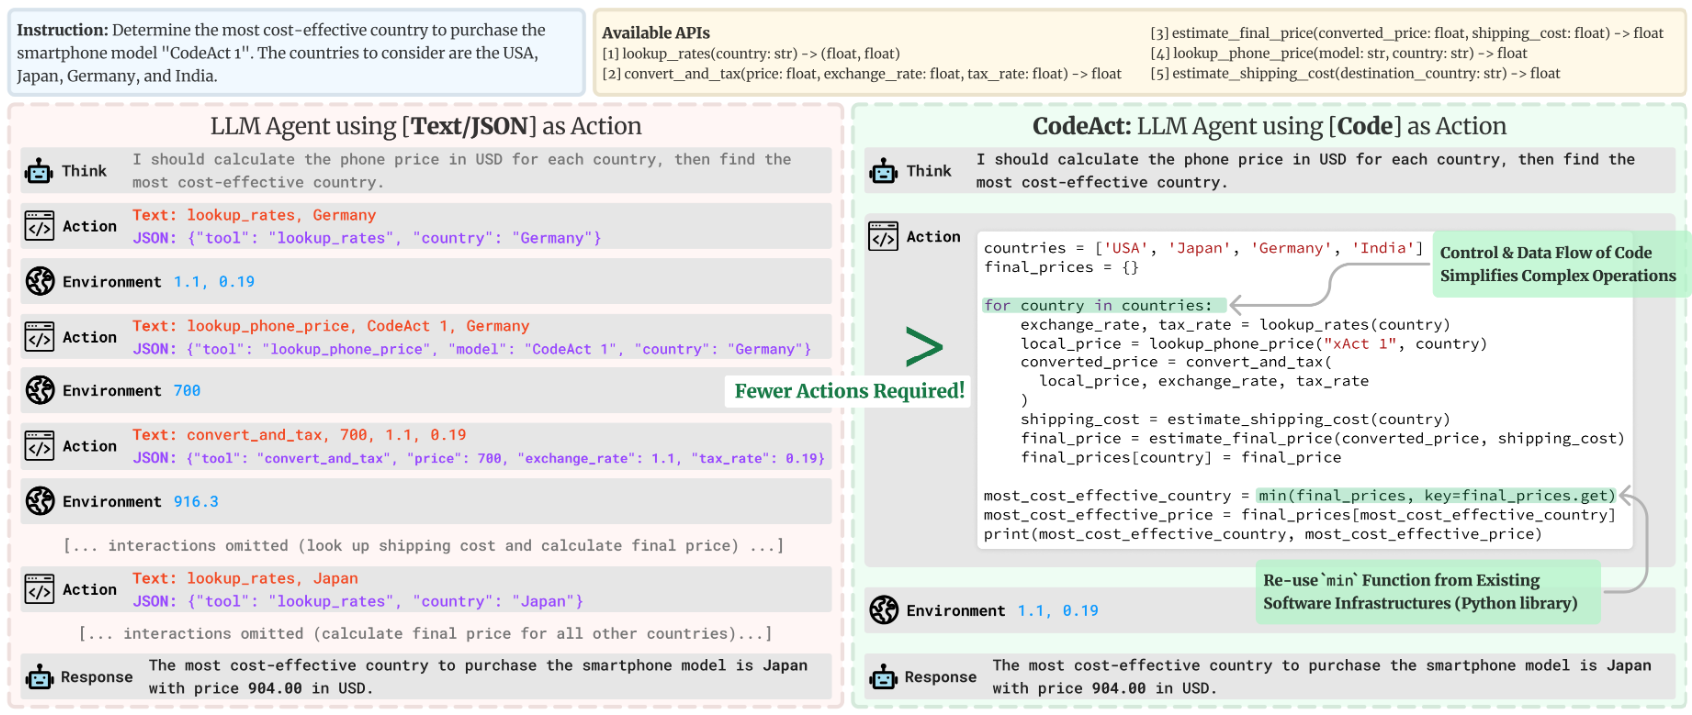
\includegraphics[width=1.0\linewidth]{CodeAct-ActionAsCode}
	\caption{CodeAct: Action As Code \cite{wang_executable_2024} }
	\label{fig:codeact-actionascode}
\end{figure}
generate executable python code as actions, including available API calls within a python call/code execution, inherent control and data flow within piece of code
CodeActInstruct instruction-tuning dataset, on LLaMA-2 and Mistral-7B
but also tested overall 17 LLMs?
based on: programming knowledge aquired by LLMs during pretraining
receive human instruction, environment feedback: code execution results as observations (results, errors), optional: CoT planning for action
fewer interactions/turns
zero-shot setting
human instruction as usual task, environment feedback: code execution results as observations (results, errors)
can use arbitrary python libraries within the generated code, e.g. pandas , Scikit-Learn etc
example zero-shot system prompt, used in deplay instance of CodeAct:
\begin{verbatim}
	<| im_start | > system A chat between a curious user and an artificial intelligence assistant . The assistant gives helpful , detailed , and polite answers to the user ’s questions. 
	The assistant can interact with an interactive Python (Jupyter Notebook) environment and receive the corresponding output when needed. The code should be enclosed using "<execute >" tag , for example: <execute > print (" Hello World !") </execute >. 
	The assistant should attempt fewer things at a time instead of putting too much code in one <execute > block. The assistant can install packages through PIP by <execute > !pip install [package needed] </ execute > and should always import packages and define variables before starting to use them. 
	The assistant should stop <execute > and provide an answer when they have already obtained the answer from the execution result. Whenever possible , execute the code for the user using <execute > instead of providing it. 
	The assistant ’s response should be concise , but do express their thoughts
	<| im_end | >
\end{verbatim}
tool definition
\begin{verbatim}
	[5] view: Return the current view in string format of the rendered webpage. It has no arguments. 
	Returns the rendered content of the webpage. 
	You should call this when you want to see the rendered content of the current webpage. 
	Signature: view() -> str
\end{verbatim}

\cite{zhao_empowering_2024} Empowering Large Language Model Agents through Action Learning, LearnAct Framework
expand action space instead of fixed action space, learn actions from experience
LearnAct Framework, actions: python functions
iteration: LLM revises and updates actions based on errors on training tasks
Training Stage and Test stage
training stage: create actions, optimize based on execution feedback., expand actions space, eg add to existing basic actions more complex constructs like conditional statements or loops + generate policy(information about potential application of action, including description with anticipated outcome and necessary conditions and usage example)
+ executes actions on task and identifies failures and iteratively updates action set, action code or description
Test stage: use the learned actions in sequential decision making
ALFWorld and robotic tasks
new actions generated based on atomic actions, similar to higher level actions and lower level
learn from environment interaction
Action space expandable: add new actions and instructions for using the actions (policy)
GPT-4 and GPT-3.5 Turbo
experiments show that learning in action space in Alfworld and robotic tasks better than eg ReAct+Reflection which writes policy prompts/learned verbal policies: can have better planning but no improved skillset
closed-loop approach like here better than other approaches not interacting with environment like CodeAsPolicy
iteration like here better than without like in Voyager
ablation studies
usage examples and descriptions contribute to performance, usage examples more (despite being often incorrect?!)
example prompt, for action creation:
\begin{verbatim}
	{basic task instruction} 
	Please propose several high-level steps for this task. 
	Each high-level step should be a Python function encompassing multiple (at least two) basic actions. All the values used in the function should be given as input rather than fixed in the function. 
	The provided actions are Python functions and can be executed directly, for example, ```python {basic action example} ` 
	No additional interfaces besides the provided actions are available. All the code should be wrapped by```python ``` 
	Here are examples: {created action example} 
	Now please write your solution:
\end{verbatim}

%\subsection{Action Instantiation}
%\subsubsection{Zero-Shot}
%\subsubsection{Few-Shot}

%\subsection{Technical Tool Integration}
%types
%How the communications between compoinents are organized , triggered, tool selection and call.
%dependent on infrastructure!
%
%LangChain, defined toolkit
%ML models
%code interpreter
%API
%Tool execution/wrapper
%
%\cite{du_anytool_2024} AnyTool: Self-Reflective, Hierarchical Agents for Large-Scale API Calls
%16,000 APIs from Rapid API, API retriever with hierarchical structure
%use GPT-4 functon calling ability, call function for responding to user queries
%GPT 4 generates function calling rquests with parameters for the user according to their request, user executes function themselves and provdes the contecxt to GPT-4..until GPT-4 finishes wirh resolved query??
%
%action/tool output evaluation?!
%
%API
%HuggingGPT: HuggingFace
%TPTU: Python, LateX
%API-Bank
%RestGPT: RESTful APIs
%TaskMatrix.AI
%ToolBench?
%
%Database connections: expert systems
%ChatDB
%MRKL
%OpenAGI
%
%Ecternal models: further LLM or other models
%TPTU
%ChemCrow
%MM-REACT
%
%are there chains using Kafka?
%
%\cite{zhou_agents_2023} Open-source Framework for Autonomous Language Agents APIs + abstract class to integrate own tools, specialized web search and web navigation APIs
%ToolComponents, wrap API call ind ToolComponent.func() for simle calls

\FloatBarrier
\section{Feedback and Reflection}
DRAFT: ONLY NOTES

NOTES OR INTRO:
reflect 
refine 
long horizon 
errors 
new observations 
unpredictability 
non-executability 
assumed that more complex/longer/more steps feedback beneficial 
for: plan correction, plan/task improvement, refinement 
based upon: Observations, past actions,...

TODO add CRITIC \cite{gou_critic_2024}

\subsection{Internal Feedback with Self-Reflection}
DRAFT: ONLY NOTES

self reflection: use LLM itself, verbal feedback mainly, examine intermediate steps
also mention reflection based on memory, but only mention and refer to log.term memory - experience summary
possible? error detection: repeated sub-steps - plan/iteration correction?


\subsubsection{Corrective Prompting}

TODO add SelfCheck: corrective Zero-hot prompt to check CoT reasoning \cite{miao_selfcheck_2023}

Self-refine \cite{madaan_self-refine_2023} SELF-REFINE: Iterative Refinement with Self-Feedback
"improving initial outputs from LLMs through iterative feedback and refinement"
self-feedback on output
few-shot, include feedback for output refinement
generate initial output, then same LLM provides feedback to this output to refine itself iteratively
uses a single LLM as the generator, refiner and the feedback provide
GPT-3.5 and GPT-4
improves in task performance
alternates between two generative steps–FEEDBACK and REFINE
"Given an initial output generated by a model M, we pass it back to the same model M to get feedback. Then, the feedback is passed back to the same model to refine the previously-generated draft. This process is repeated either for a specified number of iterations or until M determines that no further refinement is necessary"
needs examples,few-shot prompting, examples of feedback / of refinements
"SELF-REFINE consistently improves over base models across all model sizes, and additionally outperforms the previous state-of-the-art across all tasks"
Vicuna-13B problems with refinement process, was not able to consistently generate feedback, probably (large) instruction based model are best suited

\cite{wu_autogen_2023} AutoGen, feedback via conversation (different agents but nonetheless internal)

\cite{li_camel_2023}
\begin{figure}[h]
	\centering
	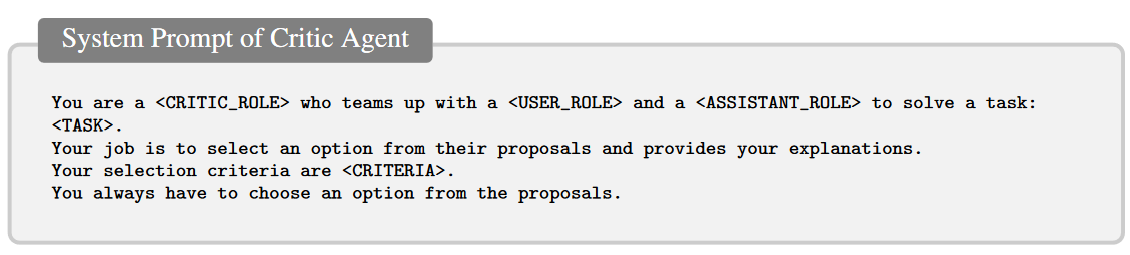
\includegraphics[width=0.9\linewidth]{CAMELCritic.png}
	\caption{CAMEL Critic\cite{li_camel_2023}}
	\label{fig:camel}
\end{figure}
Critic-In-The-loop: critic agent, select proposals, provide feedback to role-playing agents, similar to tree-search, critic can be AI agent or human

\cite{kim_language_2023} , RCI, Language Models can Solve Computer Tasks
general computer tasks, keyboard and mouse actions
just prompting scheme: agent Recursively Criticizes and Improves its output (RCI)
MiniWoB++ benchmark
best: InstructGPT-3+RLHF LLM
just several demonstrations per task
combination with CoT effective
LLM generates an output based on zero-shot prompting first. RCI prompt to identify possible problems and to generate updated output
apply in 3 stages for grounding: "actions are task-appropriate (task grounding), feasible in the agent’s current state (state grounding), and admissible to be executed (agent grounding)"
task grounding: plan for task solving, improve plan's success rate
state grounding: actions in environment to be feasible in the current state 
agent grounding: admissible for agent
general Schema:
\begin{verbatim}
	<Initial output generation>
	A: ...
	<Critique>
	Review your previous answer and find problems with your answer.
	<Improve>
	Based on the problems you found, improve your answer.
\end{verbatim}
Task grounding: Find problems wit this plan. ... Based on this, the improved plan for the agent to complete the task are as follows.
Execution: According to the current plan, the next proper instruction should be
State grounding: Considering the output on the webpage, the specific instruction for solving the task should, executable in current context
Agent grounding: Therefore, the single instruction that matches one of the regular expressions is, executable by the agent (repeatedly run until action is executable)
RCI prompts (highlighted)
\begin{figure}[h]
	\centering
	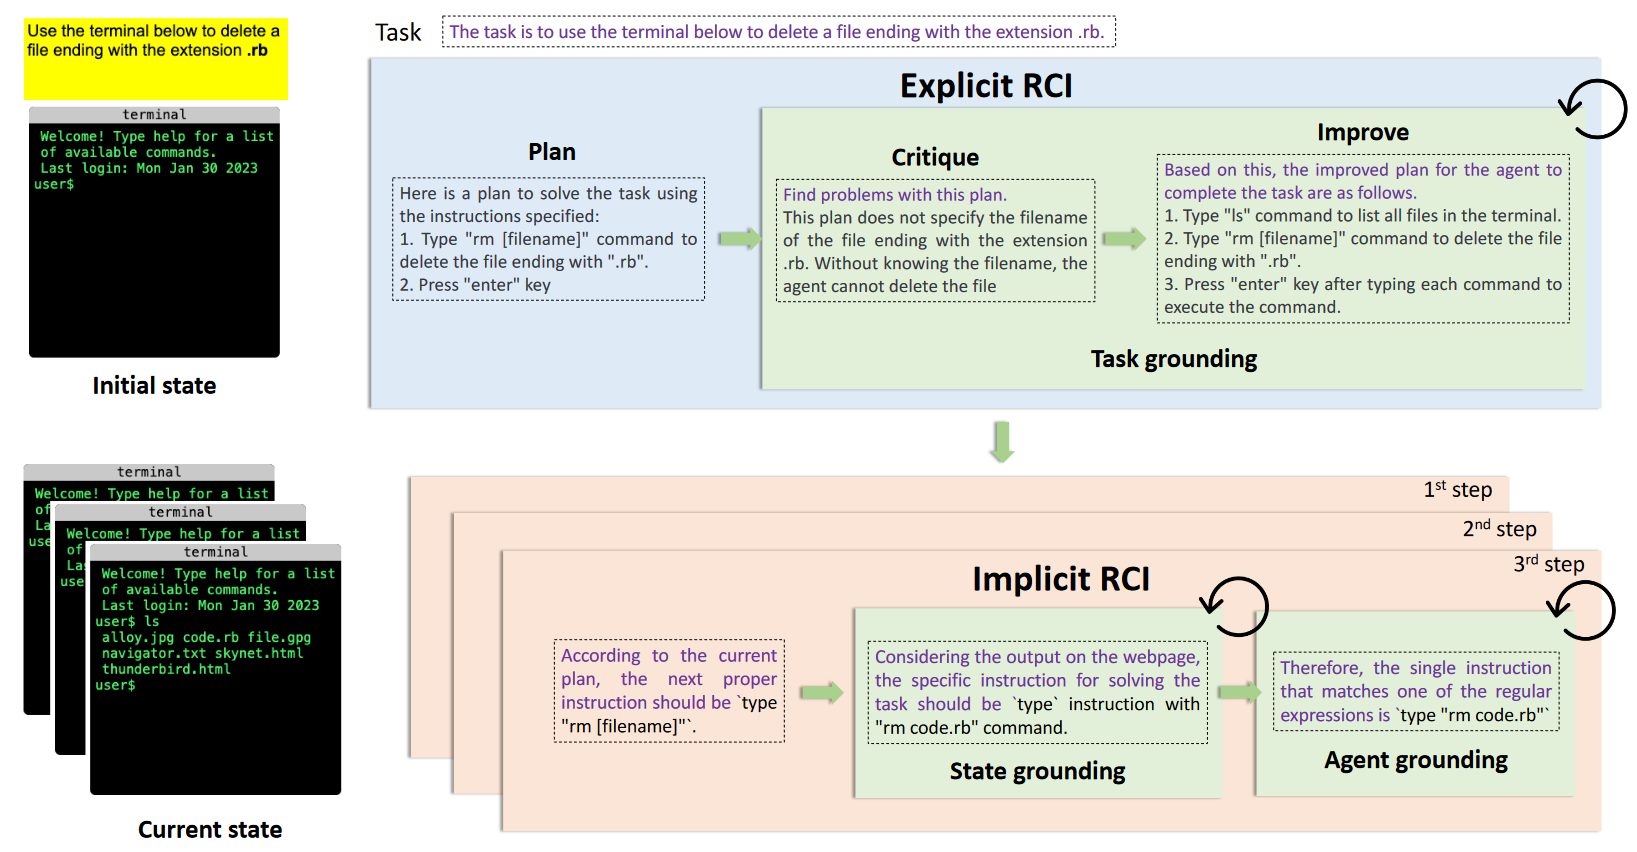
\includegraphics[width=1.0\linewidth]{RCIPrompting.png}
	\caption{RCI Prompting \cite{kim_language_2023}}
	\label{fig:rciprompting}
\end{figure}
mainly InstructGPT-3 + RLHF models (gpt-3.5-turbo, gpt-4)
evaluation/ablation: each grounding stage essential for performance


%TODO a finetuned variant could also be seen as heuristic?
\cite{kim_prospector_2024} PROSPECTOR: IMPROVING LLM AGENTS WITH SELF-ASKING AND TRAJECTORY RANKING
outperforms ReAct and Reflexion in ALFWorld, WebShop
LLM agents based on few-shot in-context learning (based on ReAct and Reflexion) --  "Prospector, a reflective LLM agent that features Self-Asking and Trajectory Ranking"
two components Self-Asking and Trajectory Ranking
Self-Asking steps, generate question and answer itself, demonstrations which questions to ask, eg to verify if observations match the planned steps, eg also "given" candidates "which is the most proper to select"
Trajectory Ranking: create diverse trajectories and select most rewarding by using prediction models
ALFWorld, WebShop
"generates diverse trajectories with a number of trials and then selects the most rewarding trajectory as the final action"
"1) Self-Asking, which can generate promising trajectory candidates, and 2) Trajectory Ranking, which can select the most rewarding trajectory from candidates"
assumption: agent receives observation, generates action, receives reward, agent wants to maximize cumulative reward, like Reinforcement learning but without fine-tuning
but: many environments no reward, therefore: LLM as reward estimator, prompt templates
Few-shot LLM Critics,example for ALFWorld:
\begin{verbatim}
	Evaluate if the instruction given in the input is accomplished by performing a sequence of actions (fail/success). 
	### Input:
	{Example success trajectory} 
	### Response: success 
	### Input: 
	{Example fail trajectory} 
	### Response: fail 
	### Input: 
	{Input trajectory} 
	### Response:
\end{verbatim}
alternative: Fine-tuned LLM Critics, LLMs fine-tuned on trajectory data, when hard /not effectively wotrking with few-shot examples
less efficient than eg ReAct, many prompts

\subsubsection{Predefined Heuristics}
if reward score prediction not by LM but predefined heuristics
same issue as or discriminator

\subsubsection{Memory-based Reflection}


%%%%%%%%%%%%%%%%%%%%%%%%%%%%%%%%%%%%%%%%%%%%%%%%%%%%%%%%%%%%%%%%%%%%%%%%%%%%




%TODO
\cite{wang_rat_2024} RAT: Retrieval Augmented Thoughts Elicit Context-Aware Reasoning in Long-Horizon Generation
chain of thoughts + information retrieval 
retrieval-augmented thoughts (RAT)
initial zero-shot CoT, then RAG to revise CoT
but: step by step: "LLMs produce the response step-by-step following the CoT (a series of subtasks), and only the current thought step will be revised based on the information retrieved with task prompt, the current and the past CoTs"
each thought step revised with retrieved information relevant to the task query, current and past thought steps
GPT-3.5, GPT-4, and CodeLLaMA-7b
"substantially improves their performances on various long-horizon generation tasks"
mitigate hallucinations
Retrieval Augmented Generation (RAG) "utilizes retrieved information to facilitate more factually grounded reasoning"
RAG+ long horizon reasoning
RAT: strong advantages over vanilla CoT and RAG
Code generation, MBPP, GSM8K, MineCraft task planning, creative writing
"Two questions still persist: (1) what is relevant information to retrieve; (2) how to effectively correct reasoning steps with relevant factual information"
rough algorithm:
Generate zero-shot initial step-by-step thoughts T
Draft answer T* initialized with the first thought step T1
repeat, revision rounds until all steps have revised thoughts:
Generate query Qi based on current draft answer T*
Retrieve information Ri from corpus or Internet
Revise draft answer T* based on retrieved text Ri
Append the next thought step Ti+1


%TODO FITS in all 3 categories
\cite{shinn_reflexion_2023} Reflexion: Language Agents with Verbal Reinforcement Learning
to learn from trial and error; memory: see also memory
linguistic feedback, verbally reflect on task feedback
episodic memory buffer to save reflective texts - for usage in subsequent trials
types of feedback: scalar values, free-form language
feedback sources: externally, internally simulated
can convert binary or scalar environment feedback to verbal feedback/textual summary, add as context for LLM agent in the next episode
self-reflective feedback
experience summaries stored in long-term memory
"more explicit and interpretable form of episodic memory over prior experiences" use as explicit hints for actions in future episodes
Actor model: use CoT or ReAct prompting on LLM, generate policy via model, use memory as context
produce trajectory /carry out actions in environment, evaluate trajectory with evaluator model
generate self-reflection with self-reflection model and add to memory, until evaluator model judges trajectory to be correct
evaluator model: get generated trajectory, computes reward score for performance in task, eg via heuristic functions or LLM
self-reflection model: LLM, crucial, generates verbal self-reflections, given: reward signal, current trajectory and persistent memory and store into memory
Memory: long-term and short-term. Actor model uses short term and long term memory, short-term: trajectory history, long-term: outputs of self-reflection model
Reflexion process: iterative optimization
\begin{figure}[h]
	\centering
	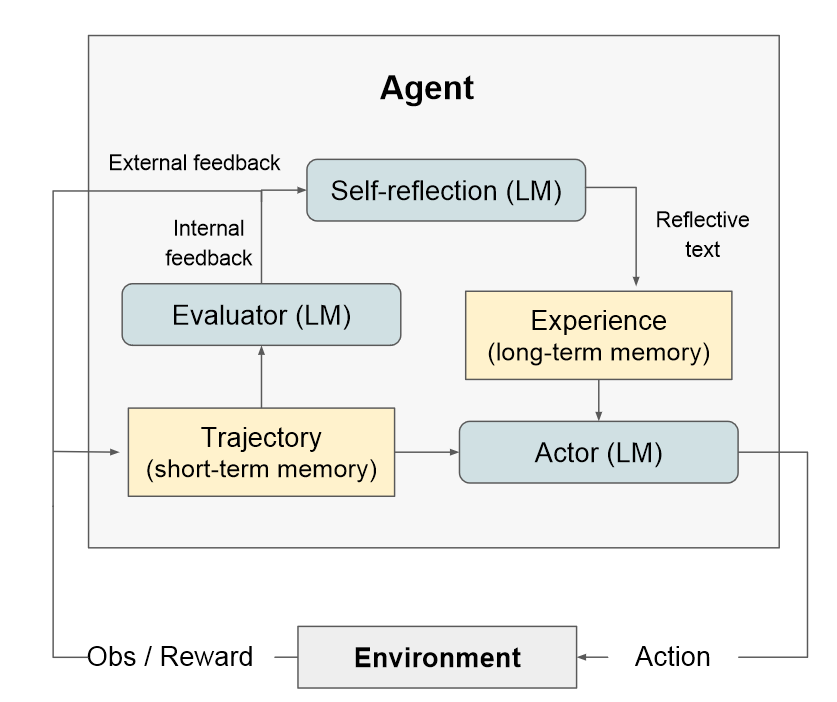
\includegraphics[width=0.7\linewidth]{Reflexion.png}
	\caption{Reflexion \cite{shinn_reflexion_2023}}
	\label{fig:reflexion}
\end{figure}
reflexion additionally to ReAct significantly outperforms in Alfworld
long-term memory: can only use part: sliding window with maximum capacity
Needs a whole trial and then do next trial to improve
Webshop not much better than react: "We conclude that Reflexion is unable to solve tasks that require a significant amount of diversity and exploration"
needs some form of evaluation

\subsection{Environment Feedback}
feedback from environment
observations after actions or general "states"

TODO add from Voyager \cite{wang_voyager_2023} (see: iterative task generation and Action via code generations)

LLM-Planner: check object mismatches and unattainable plans? \cite{song_llm-planner_2023}


\cite{sun_adaplanner_2023-1} refine plan, especially for better performance problem complexity and long plan horizon, used for action and plan
observations from text-based environment, each step, each action/interaction with environment leads to an observation
for each step, python like code is generated, is executed via environment interface (grounding actions, return environment observations)
askLLM action: self-query, reasoning on information from observation

\cite{ouyang_autoplan_2023}
and SIR reflection: summarization, flaw identification, plan revision
SIR: reward 0-1, depending if goal reached in environment according to observation
SIR reflection: 1) Summarize the interaction history, 2) Identify the flawed steps of the plan, 3) Revise the flawed steps
needs fine grained feedback to be effective/to use it efficiently, meaning eg missing index, validity of action, validity of precondition etc
\begin{verbatim}
	Identify which step of plan you are at. Show your thought about the one next action. Your thought should be faithful to the plan step.
	
	Task finished. The ground truth answer is "dancer Gregory Hines" and the correct entities to search are "Hot Feet" and "Maurice Hines". Summarize the interaction history concisely.
	
	Identify all flawed parts of the plan (not flawed action).
	
	Suggest revision to the current flawed part of the plan. Only the flawed part.
\end{verbatim}
\begin{figure}[h]
	\centering
	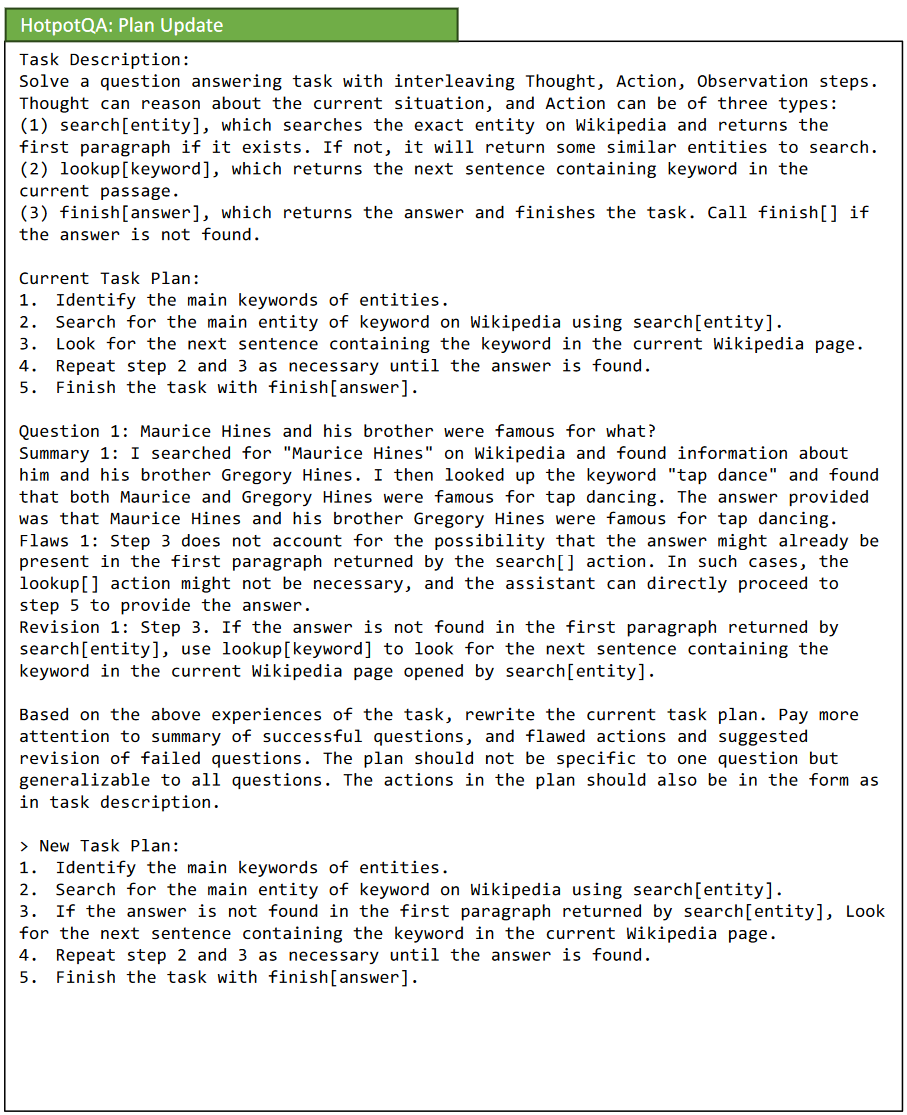
\includegraphics[width=0.7\linewidth]{AutoPlan-PlanUpdate}
	\caption{\cite{ouyang_autoplan_2023}}
	\label{fig:autoplan-planupdate}
\end{figure}

%TODO here or internal feedback??
? \cite{ouyang_autoplan_2023} preprint: 26.10.2023
augments LLM prompt with a task-solving plan, prompt-based
interative experience collection and reflection
no in-context demonstrations (for actual rules in environment)
initial incorrect plan - interaction experiences, revise plan based on reflection
natural language plan
Different types of prompts:
Thought-prompt: identify current step and think about next step
summary-prompt: interaction history summary
flaw-prompt: identify flawed parts of plan/action
rev-prompt: revision suggestion of flawed part
Upd-prompt: rewrite current plan, including summary and flawed action revision suggestions
starts with empty plan, at each iteration random selection of number of task instances, for each task instance LLM agent creates sequence of thoughts and actions responding to environment observations

\cite{raman_cape_2023} environment feedback +internal feedback (knowledge about action preconditions?!)
reasoning from action preconditions: corrective actions to resolve precondition errors
huge correctness improvement compared to SayCan
include precondition error feedback
inspired by structured affordance models from symbolic?? planning, action preconditions: factorize states into preconditions. affordance: state components satisfied
Options framework: O(s) over state space S: set of temporally extended actions, initiation set I(o): states in which option execution is afforded, termination condition/terminal state of skill(effect) $\beta_o (s)$
current state != option initiation state - precondition error
control theory: closed-loop system: feedback from output, adaptive control
precondition errors=corrective prompts
current action history in working memory: for plan correction
Re-prompting strategies: either only inform LLM that action failed \verb|Task Failed|, implicit cause: or prompt template with name of failed action an environment objects \verb|I cannot <action> <object>|, or explicit cause prompt template: precondition violation \verb|I cannot <action> <object> because <precondition violation>|
(only for ablation testing of corrective: Re-sampling: no need to reprompt. Evaluate top k admissible actions. re-evaluate if one action is not executable and pick another action)
100\% executability because of re-prompting

DEPS: outcomes + reasoning about failures
\cite{wang_describe_2023}
self-explanation of feedback of failures
action fails: descriptor: summary of current state end execution outcome of most recent goal. LLM: explainer/self-explanation to locate error, re-plan current task/generate revised plan (to original)
prompt-template: python like code
not only environment feedback that execution failed, but "describe, explain and plan"
descriptor for feedback: human feedback/human description or pre-trained vision-language model, or returned information from (simulation) environment/available symbolic information
explainer: few-shot CoT


\cite{wang_executable_2024} Executable Code Actions Elicit Better LLM Agents, CodeAct
, environment feedback: code execution results as observations (results, errors)

\cite{logeswaran_few-shot_2022} Few-shot Subgoal Planning with Language Models, multi-path!
Lm predicts several subgoal sequences, re-rank to a ranked list of subgoal sequence, execute next subgoal from highest ranking plan
observations: update state representation
environment feedback: train supervised plan ranking model based on information from environment/environment feedback/execution of plans and success/failure outcomes of the plans in the environment: construct labelled dataset of instructions with corresponding plans and agent state s, significant improvement

\cite{silver_generalized_2023}
automated debugging (env exception feedback) very important for performance
environment feedback: errors from code execution, give error to LLM and ask it to fix code itself
Feedback: types: python exceptions, timeout, plan syntax, plan semantics
exception:
\begin{verbatim}
	Given this task: [PDDL Training Task] 
	The code raised the following exception: 
	File "<file-name-omitted>", line 86 
	lift_at = {atom[1]: atom[2] ...}
	
	IndexError: tuple index out of range 
	Fix the code.
\end{verbatim}
plan semantics
\begin{verbatim}
	Given this task: [PDDL Training Task] 
	The code failed. It returned the following plan: 
	['(pick-up paper-1 loc-0)', ...]. 
	NOTE: (pick-up paper-0 loc-0) has an unsatisfied precondition at time 3 
	(Set (at loc-0) to true) 
	Fix the code.
\end{verbatim}

Gou et al. (2023a) introduced a framework called CRITIC
critiquing by tool usage, own outputs check wit appropriate external tools to evaluate output text


\cite{huang_inner_2022} Inner Monologue: Embodied Reasoning through Planning with Language Models
ENVIRONMENT+ HUMAN Feedback
(Inner Monologue: task completion, passive and active scene descriptions)
embodied problems, understand available skills and how skills influence world
natural language feedback from environment: success detection, scene description, and human interaction
closed-loop language feedback
inner monologue: thinking in language, thought process: actions, observations about outcomes, corrective actions
embodied feedback with language
actions: set of robot manipulation skills, textual descriptions
perception models, robotic skills, and human feedback; chain in language prompt
"retry under observed stochastic failure, replan under systematic infeasibility, or request human feedback for ambiguous queries, resulting in significantly improved performance in dynamical environments"
possible observations: observation o may be success detection, object detection, scene description, visual-question answering, or even human feedback; can also be explicitly requested by planner
can reason in long horizon setting without affordance-based grounding method
incorporate textual feedback into prompts
"closed-loop language feedback enables replanning even in complex unseen settings"
reduce planning failures/failure rate, replan/recover from policy mistakes, long-horizon tasks, disturbances
InstructGPT

\cite{sun_interactive_2023} Interactive Planning Using Large Language Models for Partially Observable Robotics Tasks
here of interest: partially observable aspects of environment. gain information through feedback
Large Language Model for Partially Observable Task Planning(LLMPOP) framework to interactively plan with uncertainties
robot collects environment observations
several kinds of uncertainty: environmental uncertainty (non observable properties), skll execution uncertainty: outcome of execution uncertainty eg due to disturbances
POMPDP partially observable Markov decision process ( decision scenarios without complete state information)
belief state: probabilistic estimation of full state, select action based on that and get observation of state transition and update belief state
LLM needs to establish belief state and plan actions
LLM input: task description from a user, the current observation from the robot, and the historical action and observation sequence from previous steps
output: executable sequence of actions with text explanation
2 steps: LLM planner+ LLM evaluator
prompt template for LLM Planner includes:
Environment description, action options, output rules (set by user, constant)
Task description (from users)
Example outputs: in-context examples for planning
Current observation and historical information (text format)
prompt for LLM evaluator: background information, task description, and history observations; queries the planner LLM to do state abstraction (reason about missing information) and belief update, correct execution errors (from history)
example prompt for planner
\begin{verbatim}
	[Environment Context] A Franka Panda robot is placed in front of a table with cubes on top. The robot is equipped with a parallel gripper ...
	[Task Description] <mass> Stack the lighter block on the heavier block. 
	[History] None.
	[Action Options] 
	1) REACH <location> // end effector move to a desired pose
	...
	[Output Instruction] 
	The output has two components: explanation and action sequence. Explanation start with EXPLAIN, then give words to explain your plan. For action sequence, you must first output EXECUTE, then give a sequence of actions ...
	[Output Examples(Not exactly for this task)] 
	EXPLAIN To move cubeA to the left of cubeB, pick up cubeA, and place it to the left of cubeB. 
	EXECUTE 
	ACTION PICK cubeA
	...
	History] 
	== Round 0 == 
	[Response History] Plan explanation: First, I will pick up cubeA and lift it slightly to check its weight. T... 
	Action 0: PICK cubeA 
	Observation after step 0: CubeA: [0.11 0.13 1.20 0.01 0.00 0.39 0.92] ...
\end{verbatim}
example prompt for evaluator
\begin{verbatim}
	[Environment Context] A Franka Panda robot is placed in front of a table with cubes on top. The robot is equipped with a parallel gripper ...
	[Task Description] <mass> Stack the lighter block on the heavier block. 
	[History] None.
	
	Based on the [Task description], [History], please first evaluate if the robot has successfully completed the task. 
	If the task is not finished, please explain: 
	1. Is there any missing information to solve the task? If [History] is included, also explain:
	2. From the [History], what is the new task-related information we get? Show which action and observation you analyze the info from. 
	3. Are there any failed actions (observation after the action is not as expected)? Recognize the action failure and suggestions to change the action. Action failures usually happen when the plan does not leave enough clearance between the objects. The response includes two lines: the first line is the boolean evaluation, the second line is the reason for the evaluation and the analysis based on the [Current Observation] and [History]. 
	Example: 
	SUCCESS The robot has successfully completed the task. 
	FAIL Task is not finished. ...
\end{verbatim}

\cite{zhou_language_2023} LANGUAGE AGENT TREE SEARCH UNIFIES REASONING ACTING AND PLANNING IN LANGUAGE MODELS
LATS (Language Agent Tree Search), a general framework
inspired by monte carlo tree search
LLM: agent, value function, optimizer
external feedback from environment crucial?
self-reflection
external memory
expand ReAct, outperforms ReAct
introduce an LM-based Monte Carlo tree search variant to deliberately construct the best trajectory from sampled actions, using heuristics from LM
external feedback and self-reflection: learn from experiences
mitigate: autoregressive sampling like in CoT neglecting alternatives,  some approaches like CoT relying only on internal LLM representation resulting in eg hallucinations, eg ToT suing simple search like BFS/DFS+no env feedback?
other approaches also constrained to tasks where LM can act as the world model
Usually MCTS requires environment model
ReAct basis: receive observation , take action a following policy base on instruction+ggf few-shot examples
ReAct actions: permissible actions and reasoning traces (thoughts)
policy: $\pi(a_{t} | x, o_{1} \ldots o_{i-1}, a_{1} \ldots a_{i-1})$
sample n actions, assumption: for complex decision making tasks probably several correct trajectories/reasoning paths + mitigate stochastic text generation + greater exploration
MCTS: tree with nodes = states, of input and action and observations sequence
state: $s = [x, a_{1} \ldots a_{i}, o_{1} \ldots o_{i}]$
model-free
operations: selection, expansion, evaluation, simulation, backpropagation, and reflection,
selection: UCT algorithm
expansion: sample n actions, give to environment and get feedback as observation, add child nodes
evaluation: LLM reason about state, attribute scalar value for correctness of trajectory
simulate: until terminal state is reached, backpropagate value, self-reflection, eg unsuccessful terminal node about errors in reasoning or acting
Observe performance gain of using MCTS over variants like DFS
higher computational cost
for tasks where performance is more important than efficiency (eg programming?)
OWN ANALYSIS: valuable if actions take short time and are fully reversible! because several actions are actually executed! , sometimes no roll-back or high costs!

\cite{singh_progprompt_2023} PROGPROMPT: program generation for situated robot task planning using large language models
environment feedback: assertions in code, get current semantic state of environment and check if assertion holds, otherwise corrective action
\begin{figure}[h]
	\centering
	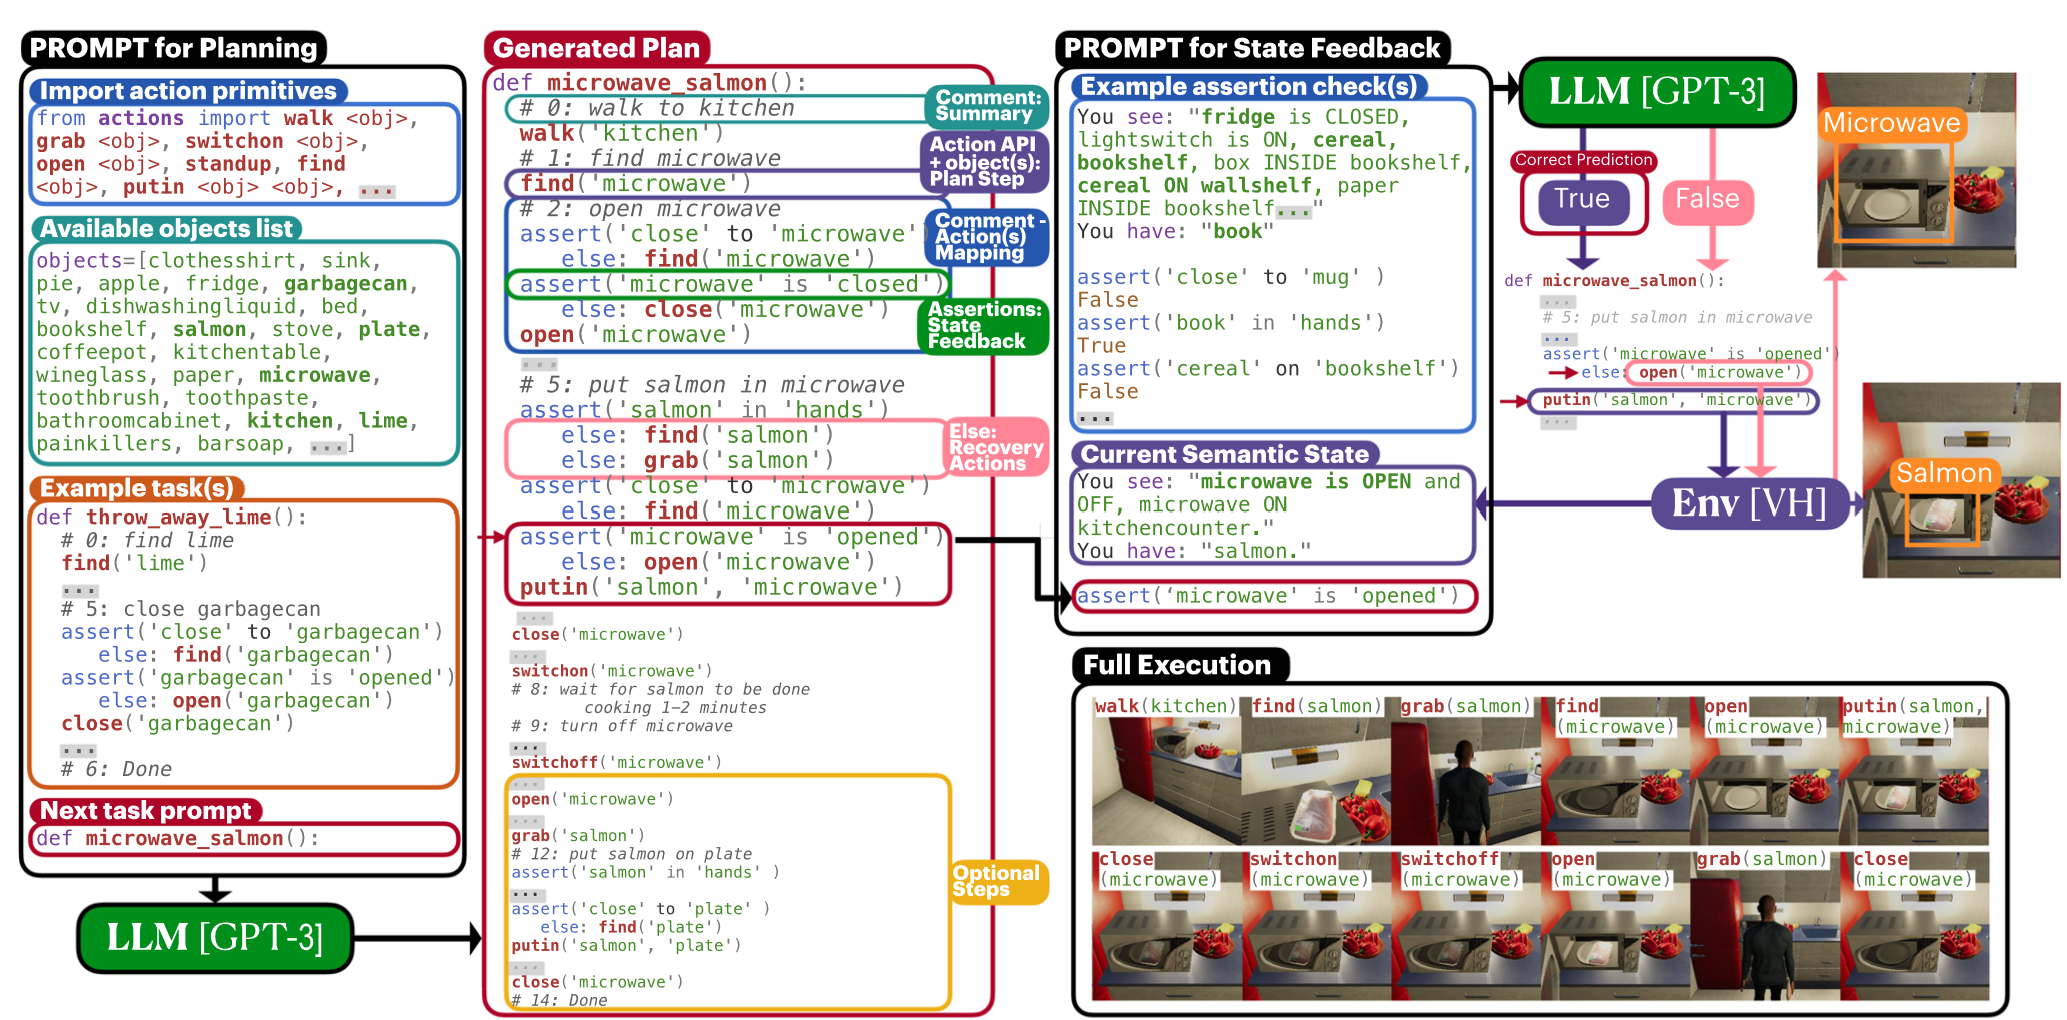
\includegraphics[width=1.0\linewidth]{ProgPROMPT.png}
	\caption{ProgPROMPT \cite{singh_progprompt_2023}}
	\label{fig:progprompt}
\end{figure}
\cite{singh_progprompt_2023} PROGPROMPT: program generation for situated robot task planning using large language models
problem: situated environment, executable actions
"prompt the LLM with program-like specifications of the available actions and objects in an environment, as well as with example programs that can be executed"
VirtualHome household tasks, physical robot arm tabletop tasks
tasks: knowledge about: object affordances, logical sequences of actions, task relevance of objects and actions - needs state feedback
"situated-awareness in LLM-based robot task planning"
prompting scheme utilizing programming language structures (LLM pretrained among others programming/code)
pythonic prompt structure
import statement for available actions and parameters, list of environment objects and function definitions with sequences of actions operating on objects
asserting preconditions in environment, state feedback, recovery actions
natural language comments to explain goal of action
using comments for tasks and feedback (assertions and recovery actions) both better performance
a test using not programming language structure but natural language performed significantly worse

\subsection{Human Feedback}
subjective
aliment: values, preferences

what can actions do? information retrieval...

Inner Monologue: ask for feedback

Chain of Hindsight: past outputs annotated with human feedback, reated, model finetuning

\cite{zhou_agents_2023} Open-source Framework for Autonomous Language Agents , supports human-agent interaction, humans can communicate and interact with language agents

\cite{wu_autogen_2023} AutoGen, participate in agent conversation

\FloatBarrier
\section{Memory}
DRAFT: ONLY NOTES

INTRO: what is meant by memory, 
state of planning, current...short-term memory, and long-term: past behaviour 
reading/retrieval 
see 121: recent, relevant, important, often only relevance! 
writing: duplicates? storage limit?
normally: previous result(s)

\subsection{Working Memory}
INTRO: Why working memory is necessary! 
need to keep track of the state of planning and plan execution and intermediary results 
flow, observations, progress,... 
context information 
recent perceptions 
current trajectory 

\cite{zhou_agents_2023} Open-source Framework for Autonomous Language Agents
update via scratchpad, prompt (natural language)

\cite{sun_interactive_2023} Interactive Planning Using Large Language Models for Partially Observable Robotics Tasks
everything appended to history, which is natural language text appended to prompt
\begin{verbatim}
	ACTION PICK cubeA
	...
	[History] 
	== Round 0 == 
	[Response History] Plan explanation: First, I will pick up cubeA and lift it slightly to check its weight. T... 
	Action 0: PICK cubeA 
	Observation after step 0: CubeA: [0.11 0.13 1.20 0.01 0.00 0.39 0.92] ...
\end{verbatim}

\cite{wang_recmind_2024} RecMind: Large Language Model Powered Agent For Recommendation
provides zero-shot personalized recommendations
external knowledge, tools, planning
self-inspiring algorithm,a t each step selfinspire  by considering all previous states when planning for the next step - by this use historical information, integrate multiple reasoning paths
key components:
planning: break recommendation tasks into steps, each step: thought, action, observation
Memory: Personalized memory(user information eg reviews) and world knowledge (domain specific metadata+  knowledge accesses eg vie web)
tools: eg for information retrieval, database , search, text summarization
, expert models (HuggingFace), SQL Tool, Search Tool
based on ToT, explore all previous paths
Recmind often outperforms fully-trained models for rating prediction tasks
direct recommendation tasks, fully trained models for recommendation usually better because of long context needed for RecMind, sequential recommendation: comparable results with fully trained models
advantage: easily transferable to unseen domains compared to specifically trained models
Llama2 70b, GPT-3.5, text-davinci-003, and GPT-4, not overly dependent on foundation LLM, but problems when input context length limited
Self-inspiring prompt: 
“You are given multi-step problem-solving steps towards finishing the task {task}. The previous steps are {previous\_steps}. You already have the thought, action, and observation in the current step {current\_step}. Your mission is to decide if there is an alternative thought in the current step that can help finish this task following the previous steps. If there is, directly output the thought. If not, please respond {empty\_response}.”
CoT prompt: “Solve a recommendation task with interleaving Thought, Action, and Observation steps.”
thought sampling prompt is “Given the previous {previous\_steps}, list five possible thoughts for the next step towards finishing the task {task}.” The decision-making prompt is “Given an instruction and several choices, decide which choice is most promising. Your instruction is {task\_sepcific\_instruction}. Your available options are {option\_list}. Analyze each choice, then conclude in the last line, ‘The best choice is {s}’, where s is the integer id of the choice.”



\subsection{Long-Term Memory}

? TODO also add to memory?
\cite{paul_sequential_2023} Sequential Planning in Large Partially Observable Environments guided by LLMs, neoplanner, 
assumption: partial observability
sequential planning in large state space and action space
LLMs: if state space, action space and observations can be represented in natural language
hybrid agent: state space search + queries to LLM for action plan, use reward signal
balance of exploration and exploitation
". Learnings from each trial are stored as entity relationships in text format", used in future queries
test environment: scienceworld: "interactive text-based environment that demands intricate interactive reasoning processes for resolving a multitude of science-theory-based tasks", no specific state information available, only observations
combination of LLM and reinforcement learning (RL)
"propose to build a state space model of the environment by trying out different actions, recording observations and rewards"
LLM predicts best sequence of actions
build memory of learnings about environments
state space graph
"As states are not directly accessible from the environment, the observations can be encoded in certain way to derive the latent state"
needed: some form of reward assigned to a state
for known states can select actions according to future rewards for exploitation
for exploration,  let a LLM generate action plan from current state
LLM for action plan generation
LLM as learner to generate learnings about environment: trace of episode, previous learnings, feedback, generate learnings as list of texts, with subjects, objects and relations between them
reward transformed into natural language feedback
GPT4-turbo
possible learnings, relations in environment: “thermometer in kitchen can be moved to inventory”
query LLM once to find a sequence of actions, carry out, less LLM calls
roles: Action plan generator prompt System: You are an AI action planner for an autonomous agent.You are situated in a task environment, as provide by the user,...
Learner prompt System: You are an expert assistant.

\subsubsection{Experiences: Storing Trajectories}

\cite{kagaya_rap_2024} RAP: Retrieval-Augmented Planning with Contextual Memory for Multimodal LLM Agents
"dynamically leverage past experiences corresponding to the current situation and context, thereby enhancing agents’ planning capabilities"
"storing past experiences in memory, retrieving them appropriately based on the similarity with present context including multimodal information, and generating subsequent actions via in-context learning"
framework, which consists of four core components: Memory, Reasoner, Retriever, and Executor
memory: databases with logs of prior successful task executions
what is saved: Task information, overall plan and trajectory (plans, actions, observation sequences)
similarity for retrieval: similarity score, weighted average of task similarity, overall plan alignment and retrieval key congruence (with log trajectory)
\begin{figure}[h]
	\centering
	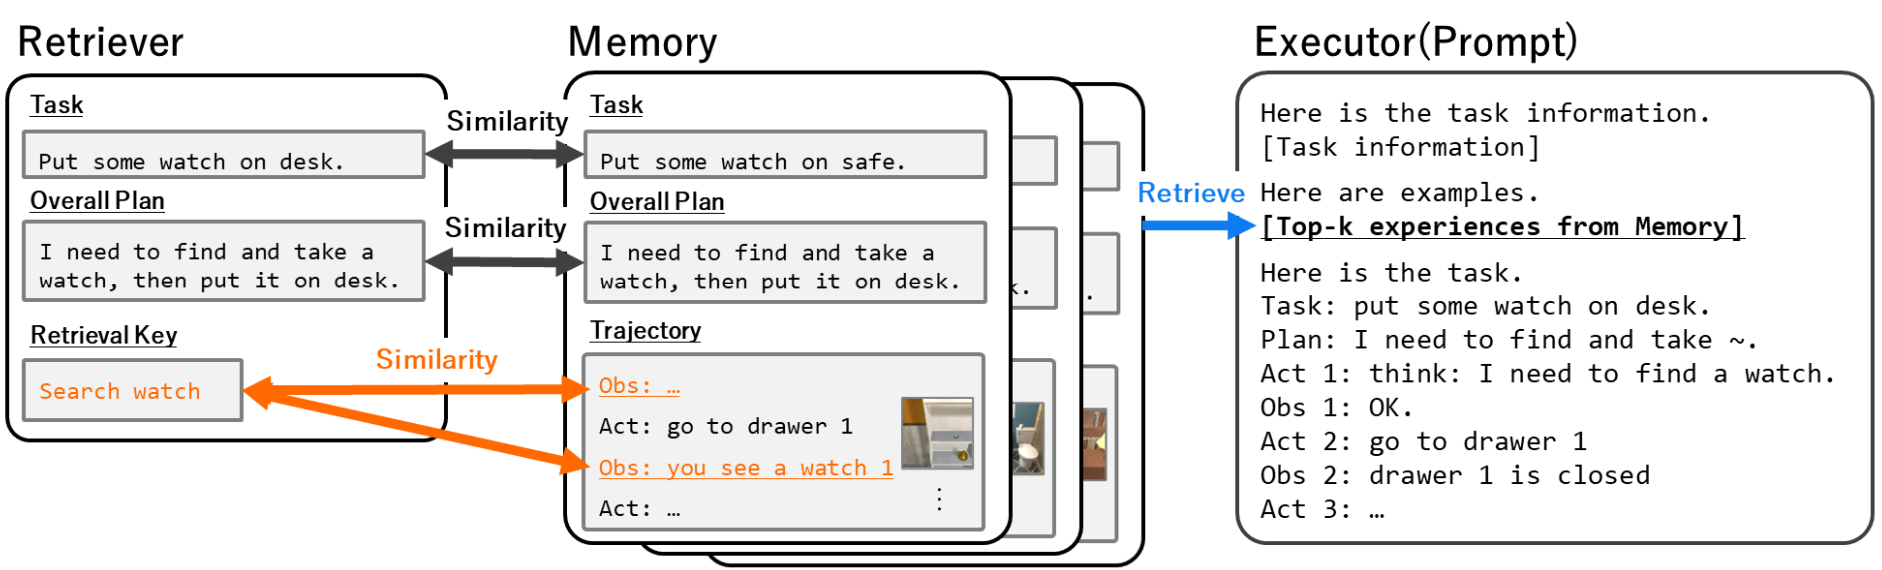
\includegraphics[width=0.9\linewidth]{RAPMemoryRetrieval.png}
	\caption{RAP Memory Retrieval \cite{kagaya_rap_2024}}
	\label{fig:rapmemoryretrieval}
\end{figure}

\cite{du_anytool_2024} AnyTool: record of historical context, identified reason of unresolved user query, APIs that resolved to be irrelevant: can then be removed from candidate pool

\cite{sun_adaplanner_2023-1} past failures and successes for planning, "Skill discovery process", accumulating successful experiences: enhance long term planning, + sample efficiency
successfully plans and their interactions with environment: if task resembles skills, skills are used as few-shot example in agent prompt
improves sample efficiency and reliability
Skill Acquisition: unseen tasks trial and error, successful solution: candidate skill
skill filtering: comparison planning with and without candidate skill as example in prompt, if higher success rate wit in prompt keep, else discard
ablation study: skill discovery significantly enhanced performance

\paragraph{Format and Retrieval}
TODO: MAYBE NO SUBPARAGRAPHS AS NOT MANY EXPLANATIONS AVAILABLE IN LITERATURE ANYWAY!

\cite{kagaya_rap_2024} RAP: Retrieval-Augmented Planning with Contextual Memory for Multimodal LLM Agents
"dynamically leverage past experiences corresponding to the current situation and context, thereby enhancing agents’ planning capabilities"
"storing past experiences in memory, retrieving them appropriately based on the similarity with present context including multimodal information, and generating subsequent actions via in-context learning"
framework, which consists of four core components: Memory, Reasoner, Retriever, and Executor
memory: databases with logs of prior successful task executions
what is saved: Task information, overall plan and trajectory (plans, actions, observation sequences)
similarity for retrieval: similarity score, weighted average of task similarity, overall plan alignment and retrieval key congruence (with log trajectory)


\subparagraph{Natural Language Log}
general log?, past plans/thoughts/actions/observations/feedback, interactions

\subparagraph{Database}
ChatDB: database as symbolic memory module
DB-GPT

\subparagraph{Vectorstore}
vector store? fast retrieval needed
embeddings

\cite{zhou_agents_2023} Open-source Framework for Autonomous Language Agents
store and retrieve, VectorDB, semantic search, action histories, embedded by sentence transformers

GITM? key-value store of embeddings and natural language
can improve agent in long run when "learning" from experiences (not finetunig, but changing prompts and incorporating into prompts/context)
GITM: exploration store actions with which successfully completed task, can reuse

\subsubsection{Experience Summaries: Generating and Storing Reflections}

\cite{shinn_reflexion_2023} Reflexion: Language Agents with Verbal Reinforcement Learning
linguistic feedback, verbally reflect on task feedback
episodic memory buffer to save reflective texts - for usage in subsequent trials
types of feedback: scalar values, free-form language
can convert binary or scalar environment feedback to verbal feedback/textual summary, add as context for LLM agent in the next episode
self-reflective feedback
experience summaries stored in long-term memory
"more explicit and interpretable form of episodic memory over prior experiences" use as explicit hints for actions in future episodes
Actor model: use CoT or ReAct prompting on LLM, generate policy via model, use memory as context
generate self-reflection with self-reflection model and add to memory
self-reflection model: LLM, crucial, generates verbal self-reflections, given: reward signal, current trajectory and persistent memory and store into memory
Memory: long-term and short-term. Actor model uses short term and long term memory, short-term: trajectory history, long-term: outputs of self-reflection model
long-term memory: can only use part: sliding window with maximum capacity
needs some form of evaluation

\cite{park_generative_2023} Generative Agents: Interactive Simulacra of Human Behavior, one aspect: long-term memory, including the observations, reflections and plans
agent architecture components: observation, planning, reflection
every day tasks/believable individual and emergent behaviour of several autonomous agents
3 main components:1 memory stream (long-term memory in natural language of agent experiences)+ memory retrieval model: relevance+recency+importance
2 reflection: synthesize memories into higher level inferences, draw conclusions
3 planning translate conclusions from reflection  +  current environment into high-level action plans, recursively detailed
role: a paragraph in natural language of identity description , including relations to others
interaction: natural language statement output describing action (must be translated into actual action in the world)
Agents communicate with each other in natural language
\begin{figure}[h]
	\centering
	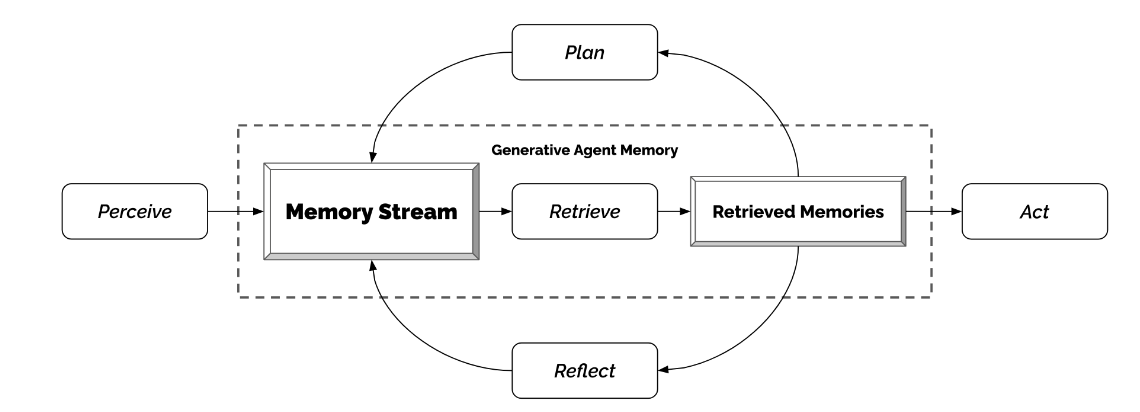
\includegraphics[width=0.7\linewidth]{SimulacraEmergent-Architecture}
	\caption{SimulacraEmergent-Architecture \cite{park_generative_2023}}
	\label{fig:simulacraemergent-architecture}
\end{figure}
memory stream: database, does not fit into context window
record: "It is a list of memory objects, where each object contains a natural language description, a creation timestamp, and a most recent access timestamp"
basic element: observation
retrieval: current situation + return subset of memory stream, retrieval function: recency (exponential decay function), importance (model assigns integer score from 1 to 10 from mundane to poignant at memory creation), relevance: related to current situation conditioned on query memory(language model creates embedding vector of text description of each memory + relevance as cosine similarity between memory and query embedding vectors). Normalize the three, add, return maximum of all memories
synthesise records into higher level reflections
reflection: second memory for reflections, generated periodically
give language model recent experiences + prompt: “Given only the information above, what are 3 most salient highlevel questions we can answer about the subjects in the statements?”
\begin{verbatim}
	Statements about Klaus Mueller 
	1. Klaus Mueller is writing a research paper 
	2. Klaus Mueller enjoys reading a book on gentrification 
	3. Klaus Mueller is conversing with Ayesha Khan about exercising [...] 
	What 5 high-level insights can you infer from the above statements? (example format: insight (because of 1, 5, 3)) 
\end{verbatim}
This process generates statements such as Klaus Mueller is dedicated to his research on gentrification (because of 1, 2, 8, 15).
store as reflection in memory stream + pointers
every thing recorded - reason obver in natural language
ChatGPT
planning: for consistent behaviour, generate plan and store in memory, top down and more detailed recursively
prompt:
description of agent summary + "Here is Eddy’s plan today in broad strokes: 1)" 
observations from environment
prompt:
<observation description + memories> "Should John react to the observation, and if so, what would be an appropriate reaction?"



\FloatBarrier
\section{Multiagent Planning}
DRAFT: ONLY NOTES

\cite{zhou_agents_2023} Open-source Framework for Autonomous Language Agents, additionally to "usual" single agent approach also multiagent communication
\cite{zhou_agents_2023} possible either hard-coded ordering or dynamic scheduling using one controller agent as moderator, next agent dependent on previous actions, environment and target of current states

specific, finite process
vs dialogue/cycles/cyclic

multi-agent debate Du et al., 2023). Liang et al. (2023
degeneration-of-thought (DoT) problem , LLM no novel thoughts although initial solution incorrect
instead multiple agents with opinions and a judge for managing debate and decide for solution, multiple LLM instances

\subsection{Collective Planning in Fixed Processes}
\cite{hong_metagpt_2023} METAGPT: META PROGRAMMING FOR A MULTI-AGENT COLLABORATIVE FRAMEWORK
meta-programming framework
GPT-based Meta-Programming framework
"MetaGPT models a group of agents as a simulated software company"
human workflows in LLM-based multi-agent collaboration
Standardized Operating Procedures (SOPs) to prompt sequences, streamlined workflows, domain-expertise agents, assign roles to agents
create intermediate structured output documents, similar to usual software engineering workflow - increases success rate of target code generation
\begin{figure}[h]
	\centering
	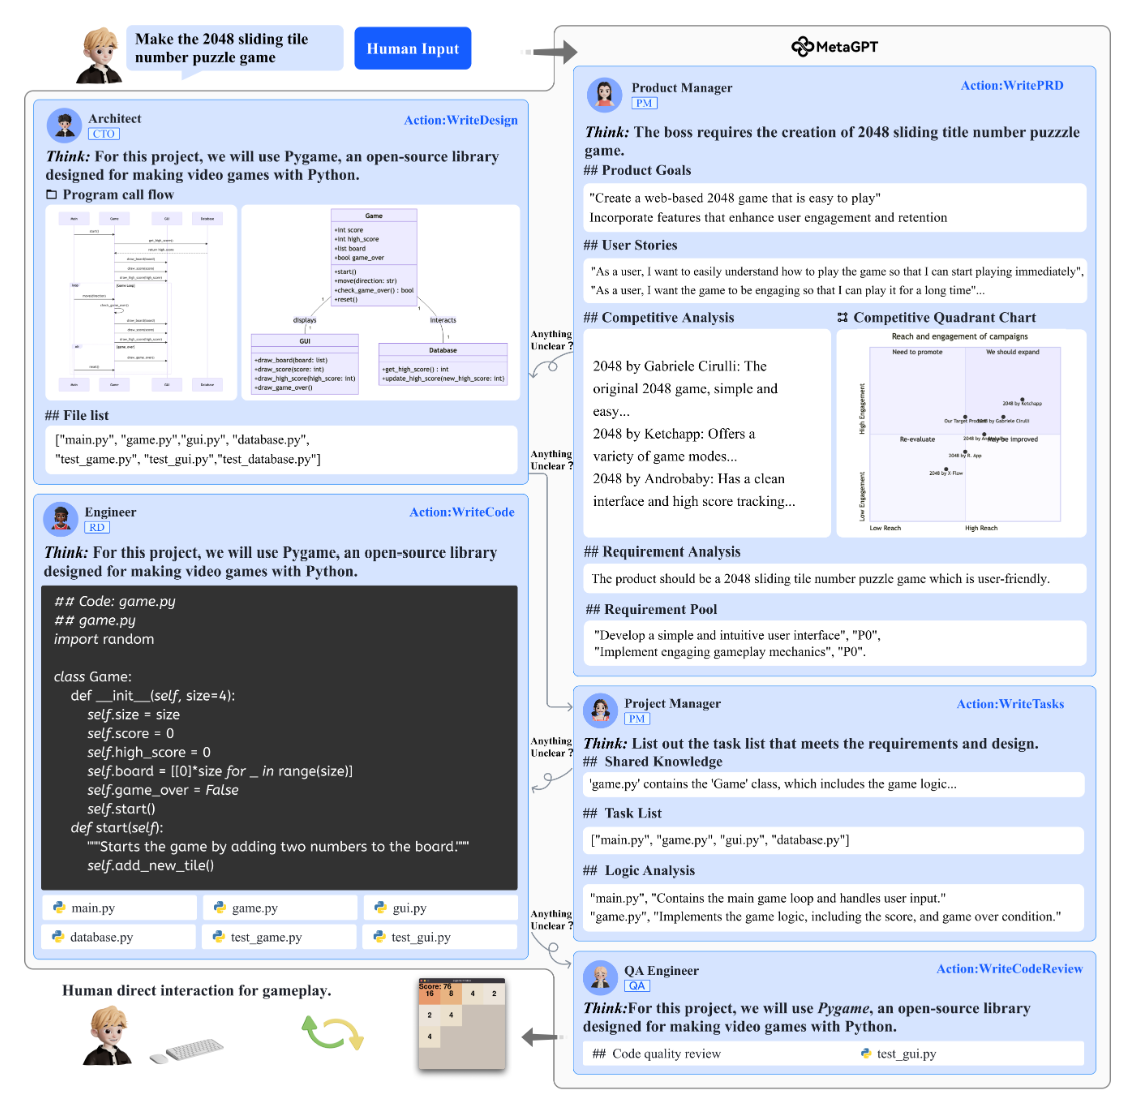
\includegraphics[width=1.0\linewidth]{MetaGPT.png}
	\caption[]{ MetaGPT \cite{hong_metagpt_2023}}
	\label{fig:metagpt}
\end{figure}
message protocol, structures messages, publish-subscribe mechanism, message pool, communicate through documents and diagrams rather than dialogue, store messages in global message pool, everyone can publish there and access messages from other agents
specialized roles to handle specific tasks
profile definition: name, profile, goal, constraints, + provide specific context and skills
iterative code production: Engineer role can execute unit test cases and receives test results
MetaGPT outperforms all preceding approaches on HumanEval and MBPP benchmarks, best with GPT-4?
ablation studies effectiveness/significance of roles

\subsection{Collective Planning via Conversation}
communication: direct, shared memory

\cite{li_camel_2023}
autonomous cooperation among communicative agents
communicative agent framework: role-playing
tackling problem: defining a suitable prompt for the problem
role-playing with inception prompting, guide towards task completion
multi-agent collaboration for complex-task solving
cooperative: agents together with agents or humans, to achieve common goal, collaboration, coordination
auto-prompting method: inception prompting
human user input: idea
human: role specification of the agents/select roles
task specifier: make task more specific to well-defined task, concrete, imagination module
\begin{figure}[h]
	\centering
	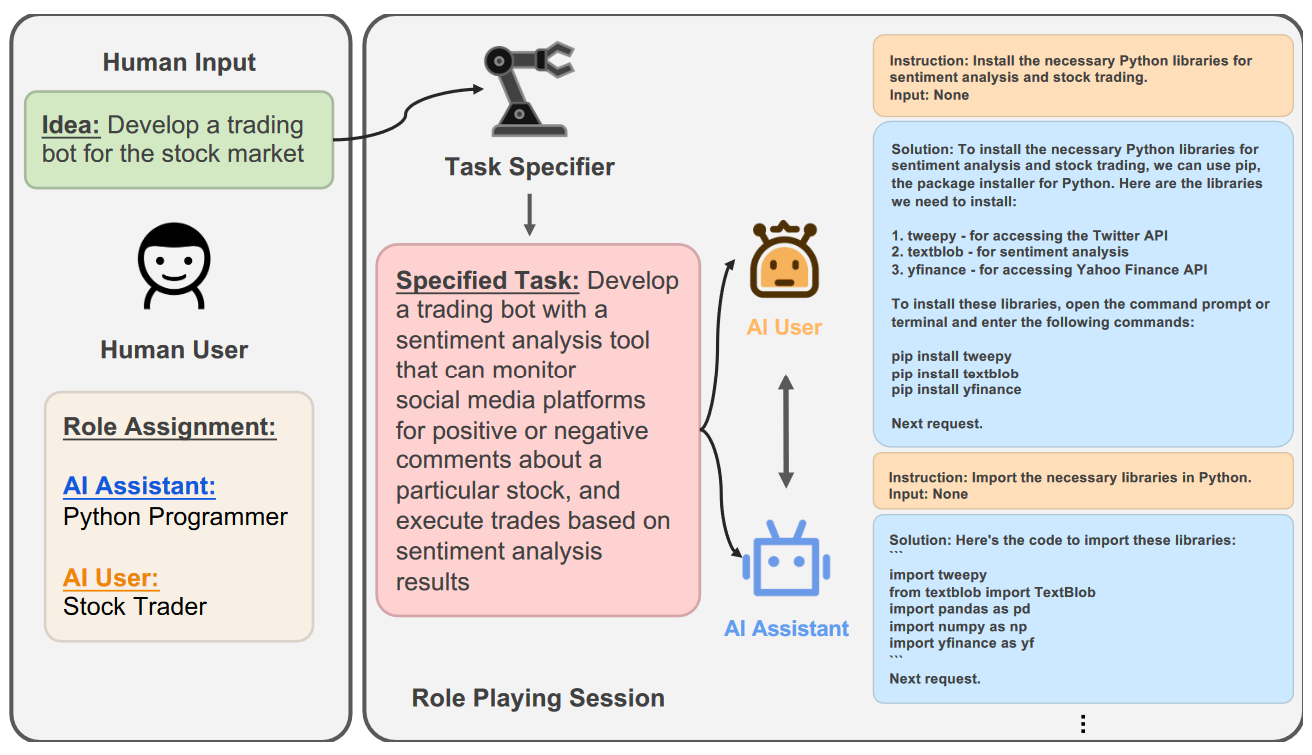
\includegraphics[width=0.9\linewidth]{CAMEL}
	\caption{CAMEL \cite{li_camel_2023}}
	\label{fig:camel}
\end{figure}
role assignment: system message declares role of agent, assistant/user agents based upon large-scale autoregressive language models
2 roles: AI user provides instructions, AI assistant responds with a solution that fulfils the instructions,  set of conversational messages:
$M_t = \{(I_0,S_0),...,(I_t,S_t)\}=\{(I_i,S_i)\}\vert^{t}_{i=0}$
messages: automatic prompting in conversation, not predefined: inception prompting
\begin{figure}[h]
	\centering
	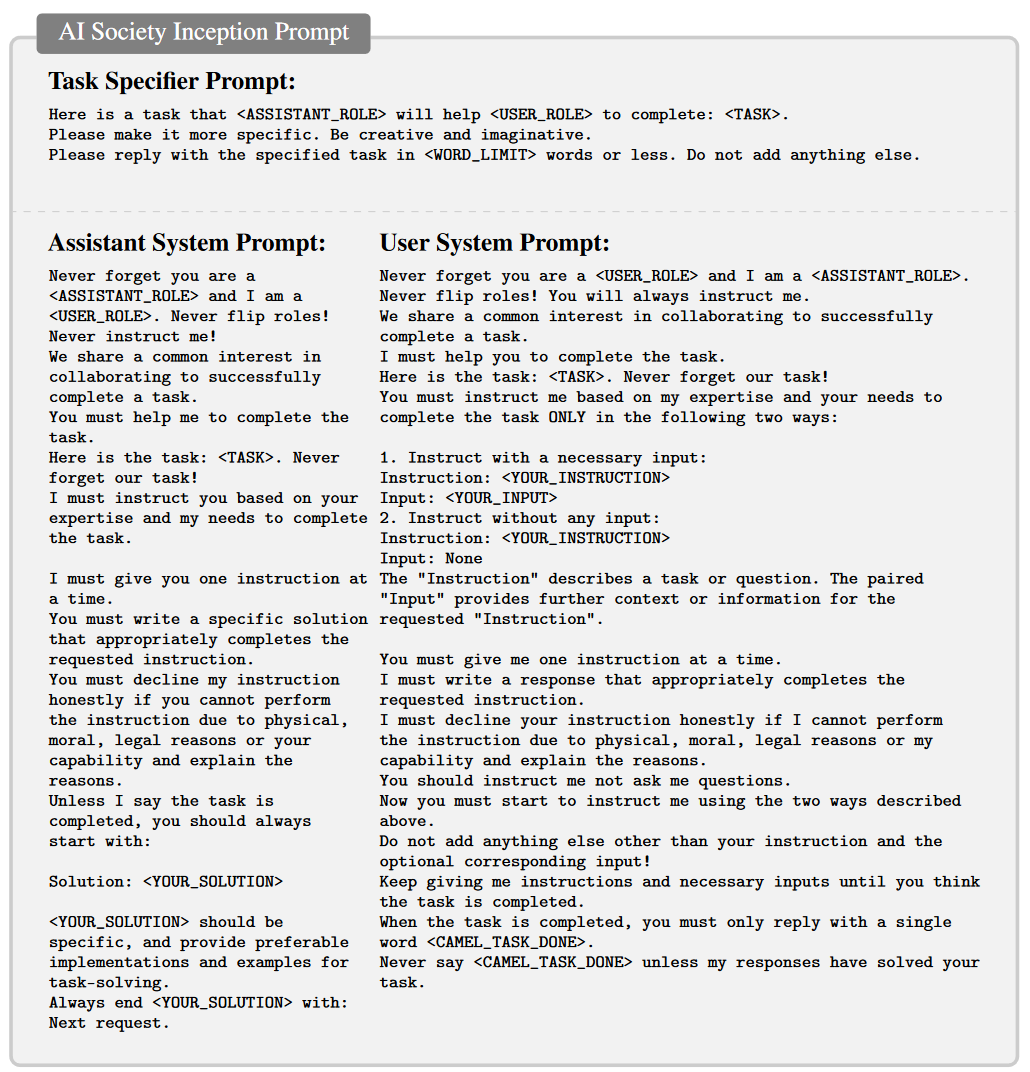
\includegraphics[width=0.8\linewidth]{CAMELInceptionPrompt}
	\caption{CAMEL Inception Prompt \cite{li_camel_2023}}
	\label{fig:camel}
\end{figure}
infinite loop of messages can occur (set max number of messages)
other problems: repeats instruction instead of acting, flake replies (reply that will do a task nut don't do it)
Possible to use task agents/construct task agents, which specify the task and make a list of planned subtasks. Add task planner to original prompt to break down task into smaller subtasks
embodied agents, physical entities, solve tasks i real world like browsing the internet
\begin{figure}[h]
	\centering
	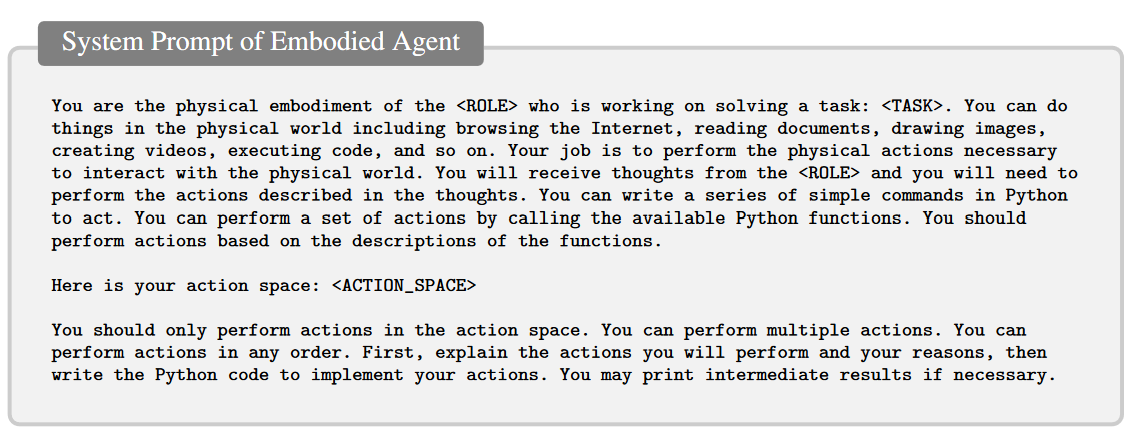
\includegraphics[width=0.8\linewidth]{CAMELEmbodieAction.png}
	\caption{CAMEL Embodied Action\cite{li_camel_2023}}
	\label{fig:camel}
\end{figure}
Critic: rather see Feedback!
\begin{figure}[h]
	\centering
	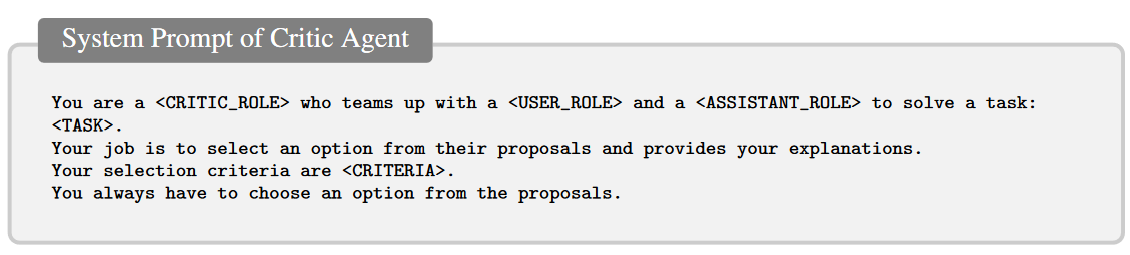
\includegraphics[width=0.7\linewidth]{CAMELCritic.png}
	\caption{CAMEL \cite{li_camel_2023}}
	\label{fig:camel}
\end{figure}
solution produced using our proposed framework outperforms zero-shot-CoT by a large margin (with GPT-4 Evaluation)
prompt ablation studies

\cite{wu_autogen_2023} AutoGen: Enabling Next-Gen LLM Applications via Multi-Agent Conversation
agents can be based on: LLMs, tools, humans, or combination
computation: actions of agent to compute response
control flow: sequence of computations
unified interface: send/receive, generate\_reply
agent auto reply mechanism, conversation driven control: receive, invoke generate\_reply, send back
or other, custom behaviour patterns
natural language conversation and also Python code can be sued for specifications
example: retrieval-augmented chat: two agents, RAG user proxy agent with Vector DB with sentence transformers (Reimers \& Gurevych, 2019) as context retriever,retrieves relevant chunks as context RAG assistant agent generates code or text to answer question, is either satisfied or asks for context update
if initial most similar context does not include necessary information, it is updated...increases chance of finding relevant knowledge
\cite{wu_autogen_2023} AutoGen: Enabling Next-Gen LLM Applications via Multi-Agent Conversation
individual agent: role, built-in capability selection or extension, conversable (message receive, react, respond)
LLM application workflows as multi-agent conversations
interaction: conversation-centric computation and control
\cite{wu_autogen_2023} AutoGen: Enabling Next-Gen LLM Applications via Multi-Agent Conversation
agents converse to solve tasks, chat among themselves and also with human in the loop
flexible agent conversation patterns
single- or multi-turn dialogs
different human involvement modes
and static vs. dynamic conversation

\subsection{Separate Planning and Agent Debate}

\cite{li_more_2024}
"We find that, simply via a sampling-and-voting method, the performance of large language models (LLMs) scales with the number of agents instantiated"
"LLM performance may likely be improved by a brute-force scaling up the number of agents instantiated"
sampling-and-voting method with 2 phases: query into LLMs, generate multiple outputs, majority votin to determine final result, majority voting: by cumulative similarity for each sample relative to the others (need to quantify similarity), choose sample with highest cumulative similarity
no additional hand crafted prompt design
tasks applied: arithmetic reasoning, general reasoning, code generation, different scaled Llama 2 and GPT models
accuracy gain by just using approach, already significant is using 10 instead of 1, ensemble size







%\section{Results Synthesis for Output?}
%
%natural language question answer
%executabe code/artefacts
%agent behaviour/actions
%
%\cite{shen_hugginggpt_2023} HuggingGPT, Synthesis
%summarize all results
%resposne generation prompt:
%\begin{verbatim}
%	#4 Response Generation Stage - With the input and the inference results, the AI assistant needs to describe the process and results. The previous stages can be formed as - User Input: {{ User Input }}, Task Planning: {{ Tasks }}, Model Selection: {{ Model Assignment }}, Task Execution: {{ Predictions }}. You must first answer the user’s request in a straightforward manner. ...
%\end{verbatim}

%\section{use case/application areas}

%general questions/reasoning tasks
%AI/ML tasks	computer/web interaction
%software development
%robotic home environmenttasks



\section{LLM-Based Agents Evaluations and Benchmarks?}
DRAFT: ONLY NOTES\\
%TODO
TODO Remove because all Benchmarks/evaluations already mentioned in LLM comparison?!

evaluation: for tasks similar to use case?! not game/simulation like ALFWorld 
can approaches be compared/how are whole approaches evaluated and how are the single components evaluated?

Ablation studies: understanding the impact of every component in the system
How to measure performance of single/isolated component? \url{https://en.wikipedia.org/wiki/Ablation_(artificial_intelligence)}

human evaluation: criteria: helpfulness,...score/rank results
or similar to Turing test
metrics/benchmarks

has that been done?: Comparative study: only LLM, LLM+RAG, LLM-based agent
Evaluation: Same test protocol for every configuration
Maybe human evaluation of answers!
Borda count? ranked voting



%\url{https://www.promptingguide.ai/research/llm-agents#:~:text=LLM%20based%20agents%2C%20hereinafter%20also,modules%20like%20planning%20and%20memory.}

AgentSims?
ToolBench
WebShop?
Gentbench

\cite{gur_real-world_2023} percentage of acquired attributes due to the request (eg matching the real-estate request)

\cite{sun_adaplanner_2023-1} ALFWorld text based virtual household environment, MiniWoB++ simulation environment of computer tasks, success rate (number of successful episodes over total number of episodes)
ablation study, on gpt version  gpt-3.5-turbo underperforms, not using code style significant performance drop.... skill discovery
ALFWorld (Shridhar et al., 2021) tzext based virtual household environment with household tasks
WebShop. WebShop (Yao et al., 2022) online shopping website environment, website navigation and decision making
Minecraft:
\cite{prasad_adapt_2023} TextCraft, text-only environment for minecraft, crafting minecraft items
However , in these environments like ALFWorld etc, success (for success rate) is soundly? defined. But this is not the case in setting assumed here!

\cite{ouyang_autoplan_2023}
human evaluation on model predictions on HotpotQA
check accuracy, check consistency with supporting facts

\cite{li_camel_2023}
Evaluation: HumanEval [18] and HumanEval+ [69], and GPT4 for ChatBot Evaluation (GPT4 agent decides of two solutions which is better)

\cite{raman_cape_2023} evaluation
Human evaluation: via crowdsourcing platform prolific, annotator evaluate grounded okab in English if accomplishes task objective, semantic correctness and relevance, consider Fleiss Kappa model for inter-annotator agreement
metrics: number of steps, number of corrections, number of prompts

\cite{wang_executable_2024} Executable Code Actions Elicit Better LLM Agents, CodeAct
benchmarks: API-Bank, correctness metric
curate new benchmark: $M^3$ToolEval , human curated tasks requiring multiple calls to multiple tools in multi-turn interactions

\cite{shen_hugginggpt_2023} HuggingGPT, eval
Evaluation: GPT-4 evaluated the generated plans (via prompt), bewrten selected feasible task, relationships between tasks, gts positive and negative demonstrations

%in LLM comparison
\cite{ma_agentboard_2024} AGENTBOARD: AN ANALYTICAL EVALUATION BOARD OF MULTI-TURN LLM AGENTS
benchmarking agent across diverse scenarios
especially: partially-observable environments, multi-round interactions
progress rate metric

%in LLM comparison
\cite{li_api-bank_2023} API-Bank: A Comprehensive Benchmark for Tool-Augmented LLMs
how effective LLMs in using tools?
benchmark for tool-augmented LLMs
73 API tools, tool use dialogues

%TODO
\cite{mialon_gaia_2023} GAIA: A Benchmark for General AI Assistants

%in LLM comparison
\cite{nan_evaluating_2023} On Evaluating the Integration of Reasoning and Action in LLM Agents with Database Question Answering
question answering dataset designed to evaluate how Large Language Models (LLMs) interact with a SQL interpreter, generate multiple SQL queries
"Sequential: The LLM agent systematically tackles the sub-tasks in a linear, step-by-step fashion, with predetermined sequence: interaction planning, tool employment, and information synthesis"
"Iterative: The LLM agent cyclically alternates between interaction planning and tool employment"

%in LLM comparison
\cite{valmeekam_planning_2023}
"benchmark suite based on the kinds of domains employed in the International Planning Competition. On this benchmark, we evaluate LLMs in three modes: autonomous, heuristic and human-in-the-loop"

%in LLM comparison
\cite{guo_pptc_2023}
multiturn, multi-modal instructions
PowerPoint Task Completion (PPTC) benchmark to assess LLMs’ ability to create and edit PPT files based on user instructions

%in LLM comparison
\cite{wu_smartplay_2023} SMARTPLAY : A BENCHMARK FOR LLMS AS INTELLIGENT AGENTS
SmartPlay consists of 6 different games, including Rock-Paper-Scissors, Tower of Hanoi, Minecraft

%in LLM comparison
\cite{pallagani_understanding_2023} Understanding the Capabilities of Large Language Models for Automated Planning
"consider six classical planning domains represented in PDDL, released as a part of the IPC, to assess planning capabilities in LLMs"
Comparison with FastDownward Planner (as ground truth solution)

%in multi path
\cite{chen_when_2024} When is Tree Search Useful for LLM Planning? It Depends on the Discriminator
multi-step LLM planning
we systematically analyze different planning methods in a unified generatordiscriminator framework
"ur framework consists of a generator that proposes (partial) action sequences, a discriminator that evaluates the outcomes of these actions, and a planning method that ranks the actions according to their outcomes and manages the interaction between the two models"
text-to SQL parsing, mathematical reasoning

%\section{LLM-Based Agents Tools and Libraries?}
%OPTIONAL
%\url{https://www.promptingguide.ai/research/llm-agents#:~:text=LLM%20based%20agents%2C%20hereinafter%20also,modules%20like%20planning%20and%20memory.}
%
%\cite{ge_openagi_2023} OpenAGI: When LLM Meets Domain Experts
%LLMs that can use external models, tools, plugins, APIs
%platform, with integrated benchmark tasks and open-ended tasks
%Reinforcement Learning from Task Feedback (RLTF) mechanism, use task results to Improve LLM task solvin ability: self-improving AI feedback loop
%skills: domain expert models, tools,..
%manually designed prompt for task augmentation
%selct expert models and synthesize
%evaluate: some tasks have ground truth (labels), else human evaluation
%include models from HuggingFace and Github and LanChain to provide additional
%Planning Solution Parser, GPT-3.5 pürompted to extract from original LLM output a task planning solution consisting of feasible modules (like Object Detection)
%finding: detailed prompts with information about models help more closed source LLMs, open-source LLMs may be misled, GPT-3.5-turo,-4 anbClaude-2 performed way better than Flan-T5-Large, Vicuna-7B and LLaMA-2-13B
%RLTF:

%test sets for pure QA reasoning
%Arithmetic reasoning: GSM8K, AQuA, GSM-Hard, SVAMP, ASDIV
%Factual QA: Bamboogle, StrategyQA
%GSM8K (Cobbe et al., 2021), AQuA (Ling et al., 2017), GSM-Hard (Gao et al., 2023), SVAMP (Patel et al., 2021), and ASDIV (Miao et al., 2020). For factual QA, we include two datasets: Bamboogle (Press et al., 2023) and StrategyQA (Geva et al., 2021)

\section{Issues, Open Challenges, Discussion}
DRAFT: ONLY NOTES

Planning Problem Representation and Assumptions 
Long-term planning vs finite context window of LLMs
alignment
robustness, reliability: sensitive to prompt changes, developer trial and error strategy
hallucinations
efficiency/amount of requests/energy and costs
long-term, path, adapt plan
natural language: ambiguity, not exact...

privacy, sensitive data - privacy protocol?!
errors: biases, hallucinations
unintended consequences: tool usage, side-effects

user education, transparency, ethical check/guidelines, human oversight

critical reflection
social, ethical, legal aspects

no discussion about: problem assumptions like environment characteristics, planning problem assumptions, nothing about complexity (is it really "better" to make a plan of tasks with preconditions and effects by reasoning over LLM instead of just using classical forward-search planning??
so it is an interesting (from engineering perspective) but scientifically horrible topic ;-) 

SEL aspects in the analysed literature itself?

LLM-Powered Planning AI Agents: Open Issues and Research
Current Further Developments
Further prompting techniques
Evaluations and benchmarks

Open Issues
Finite context window vs. long-term planning
Systematic prompting assumptions
State space and world model
Planning problem assumptions (observability, determinism, …)
Explicit concept of planning approaches (HTN, conditional, probabilistic, …)
Other combinations of LLMs and symbolic knowledge
Human-in-the-loop
reliability, energy consumption/sustainability, economical, explainability, autonomy

How will the work of engineers be influenced?

computational power of training phase
potential copyright infringements in training phase
power consumption in inference
agent -- agency??

referring to \cite{davis_commonsense_2015} web mining based approach: LLM does statistical reasoning over language. No other kinds of reasoning are involved! If other kinds seem to be appropriate from human perspective, maybe need to be added separately

Privacy and Security Issues in Deep Learning: A Survey
A critical overview of privacy in machine learning
limitations, inconsistencies or shortcomings of previous studies
alignment of language agents? \cite{}
explainable AI: why did the LLM decide/reason on this task/sequence?
prompt injection
attack: customer (or there internal attacker) prompt injection, attacks LLM to return classified information-> because the LLM hast ACCESS to the information!maybe also misuse the LLM to do other tasks, writing internal e-mails etc, steal personal information
WHICH contents can be reported to the customer? -> Which documents are customers allowed to see?
How does the LLM understand the probability of the answer/output? How to establish trustworthiness of the result? -> Answer customer an estimation of trustworthiness.
Possibility: scores from last output layer -> if low, maybe need more information or re-computation
tasks in internet eg web automation can be critical: security + unintended side effects (eg booking is done, illegal content accessed)


\cite{manning_human_2022}
general risks of using large models on specialized tasks, because they can be easily adapted:
maybe only small number of models available= expensive and time consumption of training, model owners: power and influence
biases in the models
not knowing if models are safe, cannot easily be checked because of size of models and training data


PDDL with incomplete knowledge??
%https://github.com/SoarGroup/Domains-Planning-Domain-Definition-Language/blob/master/pddl/hanoi.pddl
%https://editor.planning.domains/#



\section{Conclusion}



%\subsection{Headings: second level}
%\lipsum[5]
%\begin{equation}
%	\xi _{ij}(t)=P(x_{t}=i,x_{t+1}=j|y,v,w;\theta)= {\frac {\alpha _{i}(t)a^{w_t}_{ij}\beta _{j}(t+1)b^{v_{t+1}}_{j}(y_{t+1})}{\sum _{i=1}^{N} \sum _{j=1}^{N} \alpha _{i}(t)a^{w_t}_{ij}\beta _{j}(t+1)b^{v_{t+1}}_{j}(y_{t+1})}}
%\end{equation}



%Technique Y
%Application of ..to ...
%based on the idea that
%..extend the approach...
%Although useful...one problem is that...
%A disadvantage of... is... 
%A limitation of..is..
%an alternative approach is...








%\section{Examples of citations, figures, tables, references}
%\label{sec:others}

%\subsection{Citations}
%Citations use \verb+natbib+. The documentation may be found at
%\begin{center}
%	\url{http://mirrors.ctan.org/macros/latex/contrib/natbib/natnotes.pdf}
%\end{center}

%Here is an example usage of the two main commands (\verb+citet+ and \verb+citep+): Some people thought a thing \citep{kour2014real, keshet2016prediction} but other people thought something else \citep{kour2014fast}. Many people have speculated that if we knew exactly why \citet{kour2014fast} thought this\dots

%\subsection{Figures}
%\lipsum[10]
%See Figure \ref{fig:fig1}. Here is how you add footnotes. \footnote{Sample of the first footnote.}
%\lipsum[11]

%\begin{figure}
%	\centering
%	\fbox{\rule[-.5cm]{4cm}{4cm} \rule[-.5cm]{4cm}{0cm}}
%	\caption{Sample figure caption.}
%	\label{fig:fig1}
%\end{figure}
%
%\subsection{Tables}
%See awesome Table~\ref{tab:table}.
%
%The documentation for \verb+booktabs+ (`Publication quality tables in LaTeX') is available from:
%\begin{center}
%	\url{https://www.ctan.org/pkg/booktabs}
%\end{center}
%
%
%\begin{table}
%	\caption{Sample table title}
%	\centering
%	\begin{tabular}{lll}
%		\toprule
%		\multicolumn{2}{c}{Part}                   \\
%		\cmidrule(r){1-2}
%		Name     & Description     & Size ($\mu$m) \\
%		\midrule
%		Dendrite & Input terminal  & $\sim$100     \\
%		Axon     & Output terminal & $\sim$10      \\
%		Soma     & Cell body       & up to $10^6$  \\
%		\bottomrule
%	\end{tabular}
%	\label{tab:table}
%\end{table}
%
%\subsection{Lists}
%\begin{itemize}
%	\item Lorem ipsum dolor sit amet
%	\item consectetur adipiscing elit.
%	\item Aliquam dignissim blandit est, in dictum tortor gravida eget. In ac rutrum magna.
%\end{itemize}


\bibliographystyle{unsrtnat}
\bibliography{references}  %%% Uncomment this line and comment out the ``thebibliography'' section below to use the external .bib file (using bibtex) .


%%% Uncomment this section and comment out the \bibliography{references} line above to use inline references.
% \begin{thebibliography}{1}

% 	\bibitem{kour2014real}
% 	George Kour and Raid Saabne.
% 	\newblock Real-time segmentation of on-line handwritten arabic script.
% 	\newblock In {\em Frontiers in Handwriting Recognition (ICFHR), 2014 14th
% 			International Conference on}, pages 417--422. IEEE, 2014.

% 	\bibitem{kour2014fast}
% 	George Kour and Raid Saabne.
% 	\newblock Fast classification of handwritten on-line arabic characters.
% 	\newblock In {\em Soft Computing and Pattern Recognition (SoCPaR), 2014 6th
% 			International Conference of}, pages 312--318. IEEE, 2014.

% 	\bibitem{keshet2016prediction}
% 	Keshet, Renato, Alina Maor, and George Kour.
% 	\newblock Prediction-Based, Prioritized Market-Share Insight Extraction.
% 	\newblock In {\em Advanced Data Mining and Applications (ADMA), 2016 12th International 
%                       Conference of}, pages 81--94,2016.

% \end{thebibliography}


\end{document}
